%% ----------------------------------------
%%
%% NYU PhD thesis template.
%% Created by José Koiller 2007--2008.
%% Modified by Siddharth Krishna, 2019.
%%
%% ----------------------------------------

%% Use the first of the following lines during production to
%% easily spot "overfull boxes" in the output. Use the second
%% line for the final version.
\documentclass[12pt,draft,letterpaper]{report}
%\documentclass[12pt,oneside,letterpaper]{report}


% ----------------------------------------
% Macro to switch between draft version and final version
% ----------------------------------------

% Use or comment this to enable/disable draft version
\def\draftversion{}
\newcommand{\draftfinal}[2]{\ifdefined\draftversion#1\else#2\fi}
\newcommand{\draftonly}[1]{\draftfinal{#1}{}}
\newcommand{\finalonly}[1]{\draftfinal{}{#1}}


% ----------------------------------------
% Thesis metadata
% ----------------------------------------

%% Replace the title, name, advisor name, graduation date and dedication below
%% with your own. Graduation months must be January, May or September.
\newcommand{\thesistitle}{Scalable Blood Flow Simulations with Boundary Integral Equations}
\newcommand{\thesisauthor}{Matthew James Morse}
\newcommand{\thesisadvisor}{Professor Denis Zorin }
\newcommand{\thesisdept}{Computer Science}
\newcommand{\gradmonth}{July}
\newcommand{\gradyear}{2021}
%% If you do not want a dedication, scroll down and comment out
%% the appropriate lines in this file.
\newcommand{\thesisdedication}{To Mom and Dad.}


% ----------------------------------------
% Layout and formatting
% ----------------------------------------

% Uncomment to get a big black box to spot "overfull hboxes"
% \setlength{\overfullrule}{5pt}


%% Page layout (customized to letter paper and NYU requirements):
\RequirePackage[margin=1in, includefoot, letterpaper]{geometry}


%% Color definitions:
\RequirePackage[prologue]{xcolor}
\definecolor[named]{ThesisBlue}{cmyk}{1,0.1,0,0.1}
\definecolor[named]{ThesisYellow}{cmyk}{0,0.16,1,0}
\definecolor[named]{ThesisOrange}{cmyk}{0,0.42,1,0.01}
\definecolor[named]{ThesisRed}{cmyk}{0,0.90,0.86,0}
\definecolor[named]{ThesisLightBlue}{cmyk}{0.49,0.01,0,0}
\definecolor[named]{ThesisGreen}{cmyk}{0.20,0,1,0.19}
\definecolor[named]{ThesisPurple}{cmyk}{0.55,1,0,0.15}
\definecolor[named]{ThesisDarkBlue}{cmyk}{1,0.58,0,0.21}

% School color found from university's graphic identity site:
% http://www.nyu.edu/employees/resources-and-services/media-and-communications/styleguide.html
\definecolor{SchoolColor}{rgb}{0.3412, 0.0235, 0.5490} % purple
\definecolor{chaptergrey}{rgb}{0.2600, 0.0200, 0.4600} % dialed back a little
\definecolor{midgrey}{rgb}{0.4, 0.4, 0.4}

\usepackage{hyperref}
\hypersetup{colorlinks,
  linkcolor=ThesisDarkBlue,
  citecolor=ThesisPurple,
  urlcolor=ThesisDarkBlue,
  filecolor=ThesisDarkBlue}

%% Captions of Figures, tables
\RequirePackage[labelfont={bf,sf,small,singlespacing},
                textfont={sf,small,singlespacing},
                % justification={justified,RaggedRight},
                % singlelinecheck=false,
                margin=0pt,
                figurewithin=chapter,
                tablewithin=chapter]{caption}

%% Chapter headings, captions
\usepackage{fix-cm}
\RequirePackage[raggedright,sc]{titlesec}
\definecolor{gray75}{gray}{0.75}
\newcommand{\hsp}{\hspace{20pt}}

\titleformat{\chapter}[hang]
{\Huge\sc}
{\textcolor{SchoolColor}{\thechapter}\hsp\textcolor{gray75}{|}\hsp}
{0pt}{\Huge\sc\raggedright}
% [\textcolor{gray75}{|}\hsp\textcolor{SchoolColor}{\thechapter}]


%% The following makes chapters and sections, but not subsections,
%% appear in the TOC (table of contents). Increase to 2 or 3 to
%% make subsections or subsubsections appear, respectively. It seems
%% to be usual to use the "1" setting, however.
\setcounter{tocdepth}{2}

%% Sectional units up to subsubsections are numbered. To number
%% subsections, but not subsubsections, decrease this counter to 2.
\setcounter{secnumdepth}{3}

%% Use the following commands, if desired, during production.
%% Comment them out for final version.
%\usepackage{layout} % defines the \layout command, see below
%\setlength{\hoffset}{-.75in} % creates a large right margin for notes and \showlabels

%% Controls spacing between lines (\doublespacing, \onehalfspacing, etc.):
\usepackage{setspace}

%% Use the line below for official NYU version, which requires
%% double line spacing. For all other uses, this is unnecessary,
%% so the line can be commented out.
\finalonly{
  \doublespacing % requires package setspace, invoked above
}

%% For generating sample text.
%% Can be removed when you've replaced all \lipsum commands with your text.
\usepackage{lipsum}


% ----------------------------------------
% Comments and TODOs:
% ----------------------------------------

% Uncomment this to remove all comments
%\newcommand{\nocomments}{}

% Uncomment this to remove all TODOs
%\newcommand{\notodos}{}

% Comments and TODOs
\newcommand{\fcomment}[2]{\ifdefined\nocomments{}\else\footnote{\textcolor{red}{#1:} #2}\fi}
\newcommand{\todo}[1]{\ifdefined\notodos{}\else\textcolor{red}{TODO\ifstrempty{#1}{}{: #1}}\fi}
\newcommand{\ftodo}[1]{\ifdefined\notodos{}\else\fcomment{TODO}{#1}\fi}

% Author comments:
\newcommand{\aen}[1]{\fcomment{Matt}{#1}}


% ----------------------------------------
% User-specific packages and macros
% ----------------------------------------

%% This inputs your auxiliary file with \usepackage's and \newcommand's:
%% It is assumed that that file is called "defs.tex".
% ----------------------------------------
% Packages
% ----------------------------------------

% 
% Place here your \usepackage's. Some recommended packages are already included.
%

% Graphics:
\usepackage[final]{graphicx}
\graphicspath{{figs/}}
%\usepackage{graphicx} % use this line instead of the above to suppress graphics in draft copies
%\usepackage{graphpap} % \defines the \graphpaper command

% Uncomment this to indent first line of each section:
% \usepackage{indentfirst}

% Good AMS stuff:
\usepackage{amsthm} % facilities for theorem-like environments
\usepackage[tbtags]{amsmath} % a lot of good stuff!

% Fonts and symbols:
\usepackage{amsfonts}
\usepackage{amssymb}

% Set the fonts
\RequirePackage[T1]{fontenc}
\ifxetex
  \RequirePackage[tt=false]{libertine}
\else
  \RequirePackage[tt=false, type1=true]{libertine}
\fi
\RequirePackage[varqu]{zi4}
\RequirePackage[libertine]{newtxmath}


% For typesetting inference rules
\usepackage{mathpartir}
% \usepackage{pftools}  % A local package
\newcommand{\bmmax}{2}
\usepackage{bm}

% Formatting tools:
%\usepackage{relsize} % relative font size selection, provides commands \textsmalle, \textlarger
%\usepackage{xspace} % gentle spacing in macros, such as \newcommand{\acims}{\textsc{acim}s\xspace}

% Page formatting utility:
%\usepackage{geometry}

\usepackage{booktabs}   %% For formal tables:
                        %% http://ctan.org/pkg/booktabs
\usepackage[labelformat=simple]{subcaption} %% For complex figures with subfigures/subcaptions
                        %% http://ctan.org/pkg/subcaption
% Options to subcaption are to label and refer to subfigures as Fig 1(a) etc.
\renewcommand\thesubfigure{(\alph{subfigure})}

\usepackage[T1]{fontenc} % needed for scaling fancy fonts (?)
\usepackage[utf8]{inputenc} % not sure this is needed

\usepackage{amssymb}
%\usepackage[table]{xcolor}

% For code
\usepackage[final]{listings}
\lstset{mathescape=true}

% For code highlighting
% \usepackage{bold-extra}

% Tikz
\usepackage{tikz,pgf}
\usetikzlibrary{matrix,arrows,positioning,calc,fit,backgrounds}
\usetikzlibrary{external}
\usetikzlibrary{patterns}
\usepackage{pgfplots,import,tkz-euclide}

% To control enum item labelling/numbering
\usepackage[shortlabels, inline]{enumitem}
% To give custom item labels and reference them
\makeatletter
\newcommand{\myitem}[1][]{
  \protected@edef\@currentlabel{#1}%
\item[#1]
}
\makeatother

% To stop aligned env swallowing up []s
\usepackage{mathtools}

% To use ifstrempty
\usepackage{etoolbox}

% For math mode tables
\usepackage{array}
% A text column in array
\newcolumntype{L}{>$l<$}

% For \llbracket and \rrbracket
\usepackage{stmaryrd}

% For dashed boxes
\usepackage{dashbox}

% For big separating conjunction
\usepackage{scalerel}

% For mathpar environment
\usepackage{mathpartir}

\usepackage{xspace}
\usepackage{multirow}

% To stop citations overflowing lines
\usepackage{breakcites}

% For citet command
\usepackage{natbib}
\setcitestyle{%
    authoryear,%
    open={[},close={]},citesep={;},%
    aysep={},yysep={,},%
    notesep={, }}
\let\cite\citep

%%
%% Place here your \newtheorem's:
%%

\theoremstyle{plain}
\newtheorem{theorem}{Theorem}[chapter]
\newtheorem{conjecture}[theorem]{Conjecture}
\newtheorem{proposition}[theorem]{Proposition}
\newtheorem{lemma}[theorem]{Lemma}
\newtheorem{corollary}[theorem]{Corollary}
\theoremstyle{definition}
\newtheorem{example}[theorem]{Example}
\newtheorem{definition}[theorem]{Definition}
\theoremstyle{plain}


% ----------------------------------------
% Generic definitions
% ----------------------------------------
% Required packages: listings, tikz

% A footnote without a marker
\newcommand\blfootnote[1]{%
  \begingroup
  \renewcommand\thefootnote{}\footnote{#1}%
  \addtocounter{footnote}{-1}%
  \endgroup
}

\renewcommand{\le}{\leqslant}
\renewcommand{\ge}{\geqslant}
% \renewcommand{\emptyset}{\ensuremath{\varnothing}}
% \newcommand{\ds}{\displaystyle}

% Math stuff
\newcommand{\R}{\ensuremath{\mathbb{R}}}
\newcommand{\Q}{\ensuremath{\mathbb{Q}}}
\newcommand{\Z}{\ensuremath{\mathbb{Z}}}
\newcommand{\N}{\ensuremath{\mathbb{N}}}
\newcommand{\T}{\ensuremath{\mathbb{T}}}
\newcommand{\C}{\ensuremath{\mathbb{C}}}
\newcommand{\eps}{\varepsilon}
\newcommand{\closure}[1]{\ensuremath{\overline{#1}}}
%\newcommand{\acim}{\textsc{acim}\xspace}
%\newcommand{\acims}{\textsc{acim}s\xspace}

\newcommand{\Land}{\bigwedge}
\newcommand{\Lor}{\bigvee}
\newcommand{\es}{\emptyset}
\newcommand{\incl}{\subseteq}
\newcommand{\impl}{\Rightarrow}
\renewcommand{\iff}{\Leftrightarrow}
\newcommand{\ra}{\rightarrow}
\newcommand{\sat}{\vDash}
\newcommand{\notsat}{\nvDash}
\newcommand{\proves}{\vdash}
\newcommand{\provesIff}{\mathrel{\dashv\vdash}}
\newcommand{\boolTrue}{\top}
\newcommand{\boolFalse}{\bot}

\newcommand{\dom}{\operatorname{\mathsf{dom}}}
\newcommand{\range}{\operatorname{\mathsf{rng}}}
\newcommand{\restrict}[2]{{#1}|_{#2}}
\newcommand{\pto}{\rightharpoonup}

\newcommand{\defeq}{\coloneqq}
\newcommand{\defiff}{\vcentcolon\iff}

\newcommand{\pipe}{\triangleright}

%% Caligraphic
%\newcommand{\Aa}{{\mathcal{A}}}
%\newcommand{\Bb}{{\mathcal{B}}}
%\newcommand{\Cc}{{\mathcal{C}}}
%\newcommand{\Dd}{{\mathcal{D}}}
%\newcommand{\Ee}{{\mathcal{E}}}
%\newcommand{\Ff}{{\mathcal{F}}}
%\newcommand{\Gg}{{\mathcal{G}}}
%\newcommand{\Hh}{{\mathcal{H}}}
%\newcommand{\Ii}{{\mathcal{I}}}
%\newcommand{\Jj}{{\mathcal{J}}}
%\newcommand{\Kk}{{\mathcal{K}}}
%\newcommand{\Ll}{{\mathcal{L}}}
%\newcommand{\Mm}{{\mathcal{M}}}
%\newcommand{\Nn}{{\mathcal{N}}}
%\newcommand{\Oo}{{\mathcal{O}}}
%\newcommand{\Pp}{{\mathcal{P}}}
%\newcommand{\Qq}{{\mathcal{Q}}}
%\newcommand{\Rr}{{\mathcal{R}}}
%\newcommand{\Ss}{{\mathcal{S}}}
%\newcommand{\Tt}{{\mathcal{T}}}
%\newcommand{\Uu}{{\mathcal{U}}}
%\newcommand{\Vv}{{\mathcal{V}}}
%\newcommand{\Ww}{{\mathcal{W}}}
%\newcommand{\Yy}{{\mathcal{Y}}}
%\newcommand{\Zz}{{\mathcal{Z}}}

% Wrappers: Parens, brackets, etc
% \newcommand{\op}[1]{\operatorname{#1}}
\newcommand{\paren} [1] {\ensuremath{ \left( {#1} \right) }}
\newcommand{\bigparen} [1] {\ensuremath{ \Big( {#1} \Big) }}
% \newcommand{\bracket}[1]{\left[#1\right]}
\newcommand{\tuple}[1]{\ensuremath{\langle #1 \rangle}}
\newcommand{\abs}[1]{\ensuremath{\lvert #1 \rvert}}
% \newcommand{\set}[1]{\ensuremath{\left\{#1\right\}}}
\newcommand{\setcomp}[2]{\ensuremath{\left\{#1\;\middle|\;#2\right\}}}

% References
\newcommand{\refCh}[1]{Chapter~\ref{#1}}
\newcommand{\refSc}[1]{Section~\ref{#1}}
% \newcommand{\refSc}[1]{\S\ref{#1}}
\newcommand{\refFig}[1]{Figure~\ref{#1}}
\newcommand{\refDef}[1]{Definition~\ref{#1}}
\newcommand{\refLem}[1]{Lemma~\ref{#1}}
\newcommand{\refThm}[1]{Theorem~\ref{#1}}
\newcommand{\refAlg}[1]{Algorithm~\ref{#1}}
\newcommand{\refEx}[1]{Example~\ref{#1}}
\newcommand{\refCor}[1]{Corollary~\ref{#1}}
\newcommand{\refTab}[1]{Table~\ref{#1}}
\newcommand{\refEq}[1]{\ensuremath{(\ref{#1})}}
\newcommand{\refRule}[1]{(\ref{#1})}
\newcommand{\refApp}[1]{Appendix~\ref{#1}}

\newcommand{\tool}[1]{\textsf{#1}}
\newcommand{\code}[1]{\textnormal{\small\texttt{#1}}}
% \newcommand{\code}[1]{\text{\lstinline{#1}}}

% TODO have macros for \forall and \exists

\newcommand{\tick}{\ensuremath{\checkmark}}
\newcommand{\cross}{\text{\sffamily X}}


% ----------------------------------------
% Paper specific macros & commands
% ----------------------------------------

%% hedgehog defs
\usepackage{cleveref}
\usepackage[linesnumbered,lined,ruled,vlined,commentsnumbered]{algorithm2e}

\usepackage{enumitem}

\newlist{criteria}{enumerate}{10}
\setlist[criteria]{label*=\arabic*}

\newtheorem{heuristic}[theorem]{Heuristic}
\crefname{heuristic}{heuristic}{heuristics}
\Crefname{heuristic}{Heuristic}{Heuristics}

\crefname{criteriai}{Criterion}{Criteria}
\Crefname{criteriai}{Criterion}{Criteria}
\crefname{alg}{algorithm}{algorithms}
\Crefname{alg}{Algorithm}{Algorithms}
% Put your definitions here
% From Abtin's template
\usepackage{subcaption}
\usepackage{xifthen}
\newcommand{\mcaption}[3]{
        \ifthenelse{\isempty{#2}}
              {\caption[#1]{\small{#3} \label{#1}}}
              {\caption[#2]{{\sc #2.} \small{#3} \label{#1}}}
        }
\newcommand{\algcaption}[3]{
        \ifthenelse{\isempty{#3}}
                   {\caption[#2]{{\sc #2.} \label{#1}}}
                   {\caption[#2]{{\sc #2.} \newline\small{#3} \label{#1}}}
        }

%% bloodflow defs
\def\rbc{\abbrev{RBC}\xspace}
\def\cc{\abbrev{CC}\xspace}
\def\rbcs{\abbrev{RBC}s\xspace}
\def\cpu{\abbrev{CPU}\xspace}
\def\gpu{\abbrev{GPU}\xspace}
\def\mpi{\abbrev{MPI}\xspace}
\def\li{\abbrev{LI}\xspace}
\def\gi{\abbrev{GI}\xspace}
\def\gir{\abbrev{RGI}\xspace}
\def\lic{\abbrev{CLI}\xspace}
\def\lcp{\abbrev{LCP}\xspace}
\def\lcps{\abbrev{LCP}s\xspace}
\def\ncp{\abbrev{NCP}\xspace}
\def\stiv{\abbrev{STIV}\xspace}
\def\p4est{\texttt{p4est}\xspace}
\def\id{\abbrev{ID}\xspace}
\def\ib{\abbrev{IB}\xspace}
\def\lb{\abbrev{LB}\xspace}
\def\dpd{\abbrev{DPD}\xspace}
\def\sph{\abbrev{SPH}\xspace}
\def\skx{\abbrev{SKX}\xspace}
\def\knl{\abbrev{KNL}\xspace}
%\def\sdc{\abbrev{SDC}\xspace}
\newcommand\sdc[1][]{\abbrev{SDC\ifthenelse{\isempty{#1}}{}{\kern 1pt}#1}\xspace}
\def\emdash/{\kern 0.2em---\kern 0.2em}

\newcommand\para[1]{\paragraph*{#1}}
\newcommand\lh[1]{\emph{#1}}           % line heading, useful for itemized

\newcommand\mathbfsf[1]{\bm{\mathsf{#1}}}
\newcommand\vectord[1]{\mathbfsf{#1}}

\newcommand\vB{\vector{B}}
\newcommand\vxd{\vectord{x}}
\newcommand\vXd{\vectord{X}}
\newcommand\vY{\vector{Y}}
\newcommand\vYd{\vectord{Y}}
\newcommand\va{\vector{a}}
\newcommand\vb{\vector{b}}
\newcommand\vf{\vector{f}}
\newcommand\vfd{\vectord{f}}
\newcommand\vF{\vectord{F}}

\newcommand\dt{\ensuremath{\Delta t}}

\newcommand\slyr{single-layer\xspace}
\newcommand\dlyr{double-layer\xspace}
\newcommand\ns{near-singular\xspace}
\newcommand\gl{Gauss--Legendre\xspace}
\newcommand\bc{boundary condition\xspace}

\definecolor{clr1}{RGB}{255, 246, 39}
\definecolor{clr2}{RGB}{124, 22, 28}
\definecolor{clr3}{RGB}{84, 170, 25}
\definecolor{clr4}{RGB}{137, 230, 251}
\definecolor{clr5}{RGB}{226, 49, 39} %red
\definecolor{clr6}{RGB}{12, 59, 136}
\definecolor{clr7}{RGB}{53, 120, 120}
\definecolor{clr8}{RGB}{50, 49, 70}
\definecolor{clr9}{RGB}{255, 0, 255}
\definecolor{clr10}{RGB}{0, 0, 255}
\definecolor{clr11}{RGB}{255, 122, 122}

\definecolor{clr12}{RGB}{130, 130, 130}
\definecolor{clr13}{RGB}{180, 180, 180}
\definecolor{clr14}{RGB}{230, 230, 230}
\definecolor{plt-blue}{rgb}{0.0078,0.2980,0.7961}%blue
\definecolor{plt-orange}{rgb}{1.0000,0.6431,0.2627}%orange
\definecolor{plt-purple}{rgb}{1.0000,0.2863,0.5255}%purple
\definecolor{plt-violet}{rgb}{0.6118,0.1765,1.0000}%violet

\usepackage[export]{adjustbox}  % adjustment boxes in floats
\pgfplotsset{compat=newest}
\usepgfplotslibrary{fillbetween}
\usetikzlibrary{arrows.meta}
\usetikzlibrary{backgrounds}
\usetikzlibrary{pgfplots.groupplots}
\usetikzlibrary{plotmarks}

\newif\ifPlotTikz
\PlotTikztrue
%
\ifPlotTikz
\pgfplotsset{compat=newest}
\usepgfplotslibrary{fillbetween}
\usetikzlibrary{arrows.meta}
\usetikzlibrary{backgrounds}
\usetikzlibrary{pgfplots.groupplots}
\usetikzlibrary{plotmarks}

\pgfplotsset{plot coordinates/math parser=false}
\pgfkeys{/pgf/images/include external/.code=\includegraphics{#1}}
\tikzexternalize[prefix=figs/]
%\tikzset{external/export=false}%disable externalization

\newcommand{\includepgf}[2][1]{
\beginpgfgraphicnamed{#2}%
\tikzsetnextfilename{external-#2}%
\scalebox{#1}{\subimport{figs/}{#2.pgf}}%
\endpgfgraphicnamed%
}

%%disable hyperref in tikz figures
\makeatletter
\tikzset{
    every picture/.style={
        execute at begin picture={
            \let\ref\@refstar
        }
    }
}
\makeatother
%
\else%for ifPlotTikz
%
\newcommand{\includepgf}[2][1]{
\scalebox{#1}{\includegraphics[]{external-#2}}%
}
%
\fi%for ifPlotTikz
%%% Local Variables:
%%% mode: latex
%%% TeX-master: "thesis"
%%% End:

%% macro to define and reference terms with document
\usepackage{relsize}
\newcommand\abbrev[1]{\textsmaller{\uppercase{#1}}} %could do \textsc{\large\lowercase{#1}} or {\small\uppercase{#1}}, insert \textup to keep the letters in Roman/upright form, e.g. \abbrevformat{O\textup{\small pen}MP}

\newcommand\gmres{\abbrev{GMRES}\xspace}
\newcommand\pde{\abbrev{PDE}\xspace}
\newcommand\bvp{\abbrev{BVP}\xspace}
\newcommand\pdes{\abbrev{PDE}s\xspace}
\newcommand\ki{kernel-independent\xspace}
\newcommand\kifmm{\abbrev{KIFMM}\xspace}
\newcommand\fmm{\abbrev{FMM}\,}
\newcommand\fft{\abbrev{FFT}\,}
\newcommand\oned{\abbrev{1D}\,}
\newcommand\twod{\abbrev{2D}\,}
\newcommand\threed{\abbrev{3D}\,}
\newcommand\qbx{\abbrev{QBX}\,}
\newcommand\bie{\abbrev{BIE}\,}
\newcommand\aabb{\abbrev{AABB}\,}
\newcommand\pvfmm{\abbrev{PVFMM}\,}
\newcommand\qbkix{\texttt{hedgehog}\,}
\newcommand\pou{\abbrev{POU}\,}
\newcommand\bem{\abbrev{BEM}\,}
\newcommand\mfs{\abbrev{MFS}\,}
\newcommand\iga{\abbrev{IGA}\,}
\newcommand\wfine{\vector{w}_\text{fine}}
\newcommand\phifine{\vector{\phi}_\text{fine}}
\newcommand\Gammah{\hat{\Gamma}}
\newcommand\nystrom{Nystr\"om\xspace}


%% shortcuts (this paper) %%%%%%%%%%%%%%%%%%%%%%%%%%%%%%%%%%%%%%%%%%%%%%%%%%%%%%%%
\def\GL{Gauss-Legendre}
\def\Pex{\ensuremath{P_\mathrm{ex}}}
\def\Cex{\ensuremath{C_\mathrm{ex}}}
\def\Pnear{\ensuremath{P_\mathrm{near}}}
\def\Cnear{\ensuremath{C_\mathrm{near}}}
\def\Tree{\ensuremath{\mathscr T}}
\def\CenterSet{\ensuremath{\mathscr C}}
\def\PatchSet{\ensuremath{\mathscr P}}
\def\UnPatch{\ensuremath{{\mathscr U}_p}}
\def\UnBox{\ensuremath{{\mathscr U}_b}}
\def\CCover{\ensuremath{C_\mathrm{cover}}}
\def\BCover{\ensuremath{B_\mathrm{cover}}}
\def\Npatch{\ensuremath{N_\mathrm{patch}}}
\def\Ncenter{\ensuremath{N_\mathrm{center}}}
\def\Nbox{\ensuremath{N_\mathrm{box}}}
\DeclareMathOperator{\dist}{dist}


\newcommand\lbl[1]{\ensuremath{\mathrm{#1}}}
\newcommand\qP{{\mathcal{P}}}
\newcommand\I{{\mathcal{I}}}
\newcommand\Pfine{{\mathcal{P}_\lbl{fine}}}
\newcommand\Pcoarse{{\mathcal{P}_\lbl{coarse}}}
\newcommand\err[1]{{\eps_\lbl{#1}}}
\newcommand{\etrg}{\err{target}}
\newcommand\mrm[1]{\mathrm{#1}}
\let\vec\undefined
\let\vector\undefined
\newcommand\vector[1]  {\bm{#1}}
\newcommand\vx{{\vector{x}}}
\newcommand\hr{{\hat{r}}}
\newcommand\vg{{\vector{g}}}
\newcommand\vX{{\vector{X}}}
\newcommand\vP{{\vector{P}}}
\newcommand\vy{{\vector{y}}}
\newcommand\vd{{\vector{d}}}
\newcommand\vc{{\vector{c}}}
\newcommand\vhc{{\hat{\vector{c}}}}
\newcommand\vz{{\vector{z}}}
\newcommand\vn{{\vector{n}}}
\newcommand\vr{{\vector{r}}}
\newcommand\vsx{{\vector{s}_{\vector{x}}}}
\newcommand\vu{{\vector{u}}}
\newcommand\Cone{{C_{(1)}}}
\newcommand\Ctwo{{C_{(2)}}}
\DeclareMathOperator*{\argmin}{arg\,min}
\newcommand{\RN}[1]{%
    \textup{\uppercase\expandafter{\romannumeral#1}}%
  }
\usepackage{mathtools}
\DeclarePairedDelimiter\ceil{\lceil}{\rceil}
\DeclarePairedDelimiter\floor{\lfloor}{\rfloor}

\newcommand\Nf{\mathcal{N}_\lbl{far}}
\newcommand\Ni{\mathcal{N}_\lbl{inter}}
\newcommand\Nn{\mathcal{N}_\lbl{near}}
\newcommand\Nt{\mathcal{N}_\lbl{tot}}
\newcommand\Ninit{N_\lbl{init}}

\newcommand{\Lmx}{L_{\lbl{max}}}
\newcommand{\Lmn}{L_{\lbl{min}}}
\newcommand{\ellm}{\ell_{min}}




% ----------------------------------------
% Document header
% ----------------------------------------

%% Cross-referencing utilities. Use one or the other--whichever you prefer--
%% but comment out both lines for final version.
%\usepackage{showlabels}
%\usepackage{showkeys}



\begin{document}
%% Produces a test "layout" page, for "debugging" purposes only.
%% Comment out for final version.
%\layout % requires package layout (see above, on this same file)


%%%%%% Title page %%%%%%%%%%%
%% Sets page numbering to "roman style" i, ii, iii, iv, etc:
\pagenumbering{roman}
%
%% No numbering in the title page:
\thispagestyle{empty}
%
\vspace*{25pt}
\begin{center}
  {\Large
    \begin{doublespace}
      {\textcolor{SchoolColor}{\textsc{\thesistitle}}}
    \end{doublespace}
  }
  \vspace{.7in}

  by
  \vspace{.7in}

  \thesisauthor
  \vfill

  \begin{doublespace}
    \textsc{
    A dissertation submitted in partial fulfillment\\
    of the requirements for the degree of\\
    Doctor of Philosophy\\
    Department of \thesisdept\\
    New York University\\
    \gradmonth, \gradyear}
  \end{doublespace}
\end{center}
\vfill

\noindent\makebox[\textwidth]{\hfill\makebox[2.5in]{\hrulefill}}\\
\makebox[\textwidth]{\hfill\makebox[2.5in]{\hfill\thesisadvisor}}

\newpage


%%%%%%%%%%%%% Copyright page %%%%%%%%%%%%%%%%%%
\thispagestyle{empty}
\vspace*{25pt}
\begin{center}
  \scshape \noindent \small \copyright \  \small  \thesisauthor \\
  all rights reserved, \gradyear
\end{center}
\vspace*{0in}
\newpage


%%%%%%%%%%%%%% Dedication %%%%%%%%%%%%%%%%%
%% Comment out the following lines if you do not want to dedicate
%% this to anyone...
\cleardoublepage
\phantomsection
\addcontentsline{toc}{chapter}{Dedication}
\vspace*{\fill}
\begin{center}
  \thesisdedication
\end{center}
\vfill
\newpage


%%%%%%%%%%%%%% Acknowledgements %%%%%%%%%%%%
%% Comment out the following lines if you do not want to acknowledge
%% anyone's help...
\chapter*{Acknowledgements}
\addcontentsline{toc}{chapter}{Acknowledgments}

I would first and foremost like to thank my advisor, Denis Zorin, for his advise and guidance throughout my PhD. I would also like to thank my committee members, Georg Stadler, Marsha Berger, Michael O'Neil and Michael Overton, for their feedback on my thesis and participating as committee members.

I'm grateful for the support of Shenglong Wang at NYU HPC, who has always gone above and beyond to help the cluster users and helped me out of many last minute jams.

I must thank Nancy Wrinkle and Joan Birman, whose excitement and passion for topology has helped me to maintain my own passions.

I want to thank Michael Shelley, for many valuable discussions and the chance to work as an intern at the Flatiron Institute.
I'm similarly grateful to Harper Langston, Pierre-David Letourneau, Julia Wei, Mitchell Harris, Rich Lethin and everyone else at Reservoir Labs for a wonderful internship and the opportunity to experience research from a new perspective.

I have had the great fortune to meet and work with many wonderful people during my time at NYU.

I am deeply thankful for the guidance and support of Abtin Rahimian, for a fruitful collaboration and friendship, and for teaching me to be a proficient researcher and engineer.
I'm equally grateful for Libin Lu, who has been not only a great collaborator but a good friend.

Most importantly, I must thank my family for their love, support and unending patience.


\newpage


%%%% Abstract %%%%%%%%%%%%%%%%%%
\chapter*{Abstract}
\addcontentsline{toc}{chapter}{Abstract}

% Replace this with your abstract:
Abstract here...

%%% Local Variables:
%%% mode: latex
%%% TeX-master: "thesis"
%%% End:


\newpage


%%%% Table of Contents %%%%%%%%%%%%
\tableofcontents


%%%%% List of Figures %%%%%%%%%%%%%
%% Comment out the following two lines if your thesis does not
%% contain any figures. The list of figures contains only
%% those figures included within the "figure" environment.
\cleardoublepage
\phantomsection
\addcontentsline{toc}{chapter}{List of Figures}
\listoffigures
\newpage


%%%%% List of Tables %%%%%%%%%%%%%
%% Comment out the following two lines if your thesis does not
%% contain any tables. The list of tables contains only
%% those tables included within the "table" environment.
\cleardoublepage
\phantomsection
\addcontentsline{toc}{chapter}{List of Tables}
\listoftables
\newpage


%%%%% Body of thesis starts %%%%%%%%%%%%
\pagenumbering{arabic} % switches page numbering to arabic: 1, 2, 3, etc.


% ----------------------------------------
% Body of Thesis
% ----------------------------------------

\chapter{Introduction}
\label{chp:intro}


Microscale particulate flows play a pivotal role in many biophysical settings.
In particular, blood flows through vasculature can be modeled with reasonable accuracy by a collection of deformable particles called \textit{vesicles} suspended in a Newtonian fluid.
A clear understanding blood circulation through capillaries would shed light on important yet complex phenomena such as vasodilation, vasoconstriction, thrombosis and clotting.
The ability to simulate such flows with modern computers would provide a means to computationally investigate these phenomena with an unprecidented level of control and resolution and is a crucial milestone in the pursuit of the next generation of biological advances.
Moreover, the tools required for blood flow simulation can also be applied in other biological settings.
By simulating deterministic lateral displacement microfluidic chips , one can optimize the device geometry and avoid the typical expensive trial-and-error manufacturing process \cite{kabacaouglu2019sorting}.
By simulating intra-cellular dynamics of organelles, researchers can gain insights into biophysical dynamics by adjusting model formulations and infer biological behaviors by comparing experimental and computational results \cite{nazockdast2017cytoplasmic}. 
With better computational tools, more complex systems can be investigated computationally, rapidly increasing the pace of biological innovation.
In this work, however, we will restrict our attention to red blood cell flows through capillaries.

To faithfully simulate red blood cell flows, there are several outstanding compuatational obstacles.
The first is \textit{robustness}: can we design a set of algorithms that can handle arbtirary flows?
Typical flows are characterized by complex vascular geometry, high-volume fraction flows (>45\% in humans) and long simulation times. 
This will result in nearly-touching and potentially colliding geometries that causes many standard simulation approaches to fail; our algorithms need to handle these adversarial cases.
Another challenge is \textit{accuracy}: can we reliably control the numerical error of our algorithms?
We would like accuracy of our simulation to correspond to the accuracy of our physical model, not to the accuracy of our algorithms.
Ideally, one would hope for a single parameter that can be tuned to control the overall numerical error.

Constructing accurate and robust numerical algorithms is demanding in its own right, but as little as a microliter of human blood can contain almost four million red blood cells.
This imposes a final computational challenge: in order to simulate several microliters of blood, our algorithms must be \textit{fast} and \textit{scalable}.
Achieving algorithmic complexity proportional to the number of cells size while guaranteeing robustness and high accuracy is a tall order.
Even so, the representation of such a large simulation vastly exceeds the memory capcity of a single machine, so distributed algorithms are needed to complete the simulation in reasonable times.

\section{Contributions and Outline}
This thesis overcomes these obstacles, resulting in a practical simulation platform for realistic red blood cell flows.
In particular, this thesis will proceed as follows:
\begin{itemize}
    \item In \Cref{chp:hedgehog}, we introduce an $O(N)$ high-order solver for elliptic \pdes in \threed geometries.
        The core component of the solver is \qbkix, a straightforward \pde-independent singular/near-singular quadrature scheme for layer potentials arising from \pdes defined on domains with spline-based boundaries.
        We design addaptive geometric preprocessing and query algorithms to gurantee the accuracy of \qbkix while enabling good performance. 
        We evaluate the method on a variety of complex geometries and boundary conditions and stress test it on several challenging geometries
    \item In \Cref{chp:bloodflow}, we present a robust scalable bloodflow simulation platform. 
        We parallelize the \pde solver presented in \cref{chp:hedgehog} to scale to thousands of processors.
        We then integrate this with several parallel vesicle simulation libraries. 
        In partiular, we extend a collision-free time-stepping scheme for vesicles to also handle rigid boundaries.
        We explore strong and weak scaling results and scale this simulation to thousands of cores.
\end{itemize}

\section{Background}
\todo{physical assumptions?}
\begin{itemize}
    \item \todo{related work on low accuracy scalable blood flow}
    \item \todo{related work on BIE for blood flow}
\end{itemize}

\section{Overall Approach}
\todo{boundary integral}
\begin{itemize}
    \item Rigid boundary: qbx
    \item vesicle: shravan, abtin, dhairya etc.
\end{itemize}


% Sample content:

\chapter{Problem Formulation and Discretization}
\label{chp:formulation}

\section{Formulation\label{sec:formulation}}
\subsection{Problem Setup}

We restrict our focus to interior
%\note[DZ]{the pictures usually show an exterior problem?}
%\note[MJM]{added a comment that formulation applies to both problems}
Dirichlet boundary value problems of the form
\begin{align}
  L u(\vx) =  0,& \quad \vx \in \Omega,\\
  u(\vx) =  f(\vx),& \quad \vx \in \partial\Omega = \Gamma,
  \label{eq:pde}
\end{align}
with multiply- or singly-connected domain $\Omega$ of arbitrary genus. 
Our approach applies directly to standard integral equation formulations of exterior Dirichlet and Neumann problems; we include results for an exterior Dirichlet problem in \cref{sec:results-torii}.
Here $L$ is a linear elliptic operator and $f$ is at least $C^k$.
While our method can be applied to any non-oscillatory elliptic \pde, we use the following equations in our examples: 
\begin{equation}
  Lu =\begin{cases}
    \Delta u & \text{Laplace}\\
    \Delta u  - \nabla p, \quad \nabla \cdot u = 0 & \text{Stokes}\\
    \Delta u  + \frac{1}{1-2\nu}\nabla \nabla\cdot u & \text{Navier (linear elasticity)}\\
  \end{cases}
  \label{eq:pdes}
\end{equation}

We follow the approach of \cite{YBZ}. 
We can express  the solution at a point $\vx \in \Omega$ in terms of the double-layer potential
\begin{equation}
  u(\vx) = D[\phi](\vx) = \int_\Gamma \frac{\partial G(\vx,\vy)}{\partial \vn(\vy)} \phi(\vy) d\vy_\Gamma,
  \label{eq:double_layer}
\end{equation}
where $G(\vx,\vy)$ is the \textit{fundamental solution} or \textit{kernel} of \cref{eq:pde}, $\vn(\vy)$ is the normal at $\vy$ on $\Gamma$ pointing into the exterior of $\Omega$, and $\phi$ is an unknown function, or \textit{density}, defined on $\Gamma$.
We list the kernels associated with the \abbrev{PDE}s\xspace in \cref{eq:pdes} in \cite[Section 1]{morse2020bsupplementary}.
Using the jump relations for the interior and exterior limits of $u(\vx)$ as $\vx$ tends towards $\Gamma$ \cite{K,mikhlin2014integral,pozrikidis1992boundary,parton1982integral}, we know that \cref{eq:double_layer} is a solution to \cref{eq:pde} if $\phi$ satisfies 
\begin{equation}
  \left(\frac{1}{2}I + D + M\right)[\phi](\vx) = f(\vx), \vx \in \Gamma
  \label{eq:int-eq}
\end{equation}
with identity operator $I$. 
We will refer to $\phi$ as the \textit{density} and $u(\vx)$ as the \textit{potential} at $\vx$.
The double-layer integrals in this equation are \textit{singular}, due to the singularity in the integrand of \cref{eq:double_layer}. 
Additionally, as $\vx$ approaches $\Gamma$, \cref{eq:double_layer} becomes a \textit{nearly singular} integral.

The operator $M$ completes the rank of $\frac{1}{2}I + D$ to ensure invertibility of \cref{eq:int-eq}. 
If $\frac{1}{2}I + D$ is full-rank, $M = 0$.
When $\frac{1}{2}I + D$ has a non-trivial null space, $M$ accounts for the additional constraints to complete the rank of the left-hand side of \cref{eq:int-eq}.
For example, for the exterior Laplace problem on $\ell$ multiply-connected domains, the null space of $\frac{1}{2}I + D$ has dimension $\ell$ \cite{ST}.
The full set of cases for each kernel is considered in this work and their corresponding values of $M$ have been detailed in \cite{YBZ}. 

%We assume that $f(\vx)$ is $C^k$ on $\Gamma$, since the convergence order of our integration scheme depends on smoothness of $f$.
%This implies that the convergence order is at most $k$ (see \cref{sec:quad_error}).


\subsection{Geometry representation \label{sec:geom-def}}

\begin{figure}[!htb]
  \centering
  %\setlength\figureheight{1.9in}
  %\setlength\figurewidth{2.1in}
  \begin{minipage}{\textwidth}
      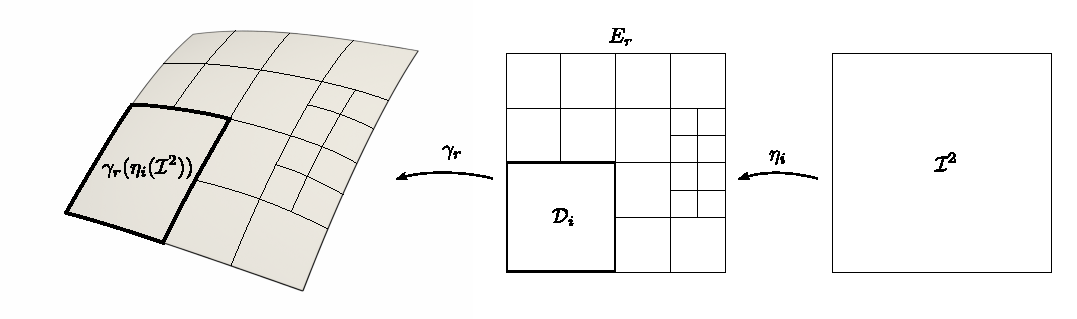
\includegraphics[width=\linewidth]{figs/quadrisection.pdf}
  \end{minipage}\hfill
%  \mcaption{fig:geometry-representation}{Patch Quadrisection}{
%      Right: the standard domain $\mathcal{I}^2$ of a single surface or quadrature patch.
%    Middle: a collection of subdomains $\mathcal{D}_i$ of $E_r$, produced by quadrisection. 
%    Each $\mathcal{D}_i$ corresponds to a map $\eta_i$ such that $\mathcal{D}_i = \eta_i(\mathcal{I}^2)$; a single $\mathcal{D}_i$ is highlighted in bold.
%    Left: the image of $E_r$ under the patch $\gamma_r$. 
%    The final image of each subdomain is outlined, with the image of $\mathcal{D}_i$ in bold.
%  }
\end{figure}
We assume that the smooth domain boundary $\Gamma$ is given by a \textit{quadrilateral mesh} consisting of quadrilateral faces $Q_r$, referred to as \textit{quads}.
Each quad is associated with a parametric domain $\I^2 =  [-1,1]^2 = E_r$, along with embeddings $\gamma_r : E_r \to \mathbb{R}^3$ for each quad such that $Q_r = \gamma_r(E_r)$.  
We assume that the quad mesh is \textit{conforming}, i.e., two non-disjoint faces either share a whole edge or a single vertex; examples of this are shown in \Cref{fig:greens-id-test-cases,fig:solver-conv-test-cases}.
We assume that no two images $\gamma_r(E_r)$ intersect, except along the shared edge or vertex.
The surface $\Gamma$ is the union of patches $\cup_r \gamma_r(E_r) = \cup_r Q_r$.
We also assume that $\Gamma$ is sufficiently smooth to recover the solution of \cref{eq:pde} up to the boundary \cite{K} and is at least $C^k$. 

To represent the surface geometry, we approximate $\Gamma$ with a collection of \emph{B\'ezier patches}, given by a linear combination of tensor-product Bernstein polynomials
\begin{equation}
    \vP_i(s,t) = \sum_{\ell =0}^n\sum_{m =0}^n \vector{a}^{(i)}_{\ell m }B_\ell^n(s)B_m^n(t),
  \label{eq:tensor-product}
\end{equation}
where  $B_\ell^n(t) = \binom{n}{\ell} t^{n-\ell}(1-t)^{\ell}$ for each $\ell$ are the $n$-th degree Bernstein polynomials, $i$ denotes the index of a patch in the collection and $\vector{a}_{\ell m}^{(i)} \in \mathbb{R}^3$.
Each patch $\vP$ is a vector function from $\I^2$ to $\mathbb{R}^3$, so $s,t\in [-1,1]$.
We will refer to this approximation of $\Gamma$ as $\hat{\Gamma}$. % and detail its construction in \cref{sec:admissible}.
%More specifically, we use a \emph{forest of quad trees of B\'ezier patches}. 

The domain $E_r$ of each embedding function $\gamma_r$ is adaptively refined using \emph{quadrisection}, i.e., splitting a square domain into four square subdomains of equal size. %This yields a quad tree of subdomains for each face of the quad mesh.
Quadrisection induces a \textit{quadtree} structure on each $E_r$. 
The root of the quadtree is the original domain $\I^2$ and each node of the tree is related by a single quadrisection of a subdomain of $E_r$. 
The leaves of the quadtree form a collection of subdomains $\mathcal{D}_i$ whose union equals $E_r$, as shown in \cref{fig:geometry-representation}-middle.
Given an indexing scheme of all $\mathcal{D}_i$'s over all $E_r$'s, we define the function $r(i)$ that maps the leaf node index $i$ to its root node index $r$ in the quadtree forest, indicating that $\mathcal{D}_i \subset E_r$. 
For each $r$, $E_r$ can have a distinct sequence of associated quadrisections and therefore a distinct quadtree structure.
We refer to the process of \textit{refinement} or \textit{refining a patch $\vP$} as the construction of such quadtrees for each $E_r$ subject to some set of criteria.

On each $\mathcal{D}_i$ at the quadtree leaves, we define a B\'ezier patch and reparametrize each patch over $\I^2$ by defining the affine map $\eta_i: \I^2 \to E_{r(i)}$ such that $\eta_i(\I^2) = \mathcal{D}_i \subseteq E_{r(i)}$.
%On each $\mathcal{D}_i$ at the quadtree leaves, we define a \emph{B\'ezier patch} given by a linear combination of  tensor-product Bernstein polynomials on $\mathcal{D}_i$:
%\begin{equation}
%    P(s,t) = \sum_{\ell =0}^n\sum_{m =0}^n \vector{a}_{\ell m }B_\ell^n(s)B_m^n(t),
%  \label{eq:tensor-product}
%\end{equation}
%where  $B_k^n(t) = \binom{n}{k} t^{n-k}(1-t)^{k}$ is $n$-th degree Bernstein polynomials.
It follows that the set of subdomains $\{ \eta_i(\I^2) \,| \,r(i) = \kappa\}$ form a cover of $E_\kappa$ and $\{ \gamma_\kappa(\eta_i(\I^2))\, | \,r(i) = \kappa\}$ likewise covers $\gamma_\kappa(E_\kappa)$.
We summarize this setup in \Cref{fig:geometry-representation}; examples of surfaces of this form can be seen in \Cref{fig:greens-id-test-cases,fig:solver-conv-test-cases,fig:torii,fig:vessel}.
%Since we have made no assumptions on the explicit form of $\gamma_r$, this approximation stage constructs a consistent surface representation that we can leverge in our algorithms in \cref{sec:admissible} without sacrificing geometric fidelity.
%At each step of quadrisection, there is a parent-child relationship formed between the subdomain and its four resulting subdomains. 
%In \Cref{fig:geometry-representation}-right, we have a single leaf of this quadtree, denoted $D_i$.

%The coefficients or \emph{control points} $\vector{a}_{\ell m}$ in \cref{eq:tensor-product} are computed to fit the B\'ezier patches to the input embeddings $\gamma_r$.
%Each patch $P_i$ in $\Pcoarse$ is reparametrized on $\I^2$ and each domain is associated with a leaf of the forest of quad trees.
%We refer to the domain of $P_i$ by $D_{i}$, noting that $D_i = \I^2$. 
%Each such domain $D_i$ corresponds to a subdomain of $E_{r(i)}$, where $r(i)$ is the index of the embedding $\gamma_{r(i)}$ from which
%$P_i$ was obtained by refinement.
%Define the  map $\eta_i: D_i \rightarrow E_{r(i)}$, which embeds the domain $D_i$ into the copy of $\I^2$ corresponding to $\gamma_{r(i)}$. 
%The set of maps $\{\eta_i \mid r(i) = k\}$ cover $\I^2$ for each embedding map $\gamma_k$.
%We summarize this setup in \cref{fig:geometry-representation}.

%In the simplest case, the input is already in B\'ezier form and no additional processing is necessary; the overall accuracy of our method is limited by therefore by the smoothness of the given polynomial surface.
%In general, $\Gamma$ can be defined by arbitrary functions. 
%The domain on which the complete approximate surface $\hat{\Gamma}$ is defined is the union of $E_{r(i)}$ identified along shared edges. 
%The complete set of B\'ezier patches defined on these domains is denoted $\Pcoarse$.

\subsection{Problem discretization \label{sec:discretization}}
We use two collections of patches in the form described above: $\Pcoarse$ and $\Pfine$.
The patches in $\Pcoarse$, called \emph{surface patches}, determine $\Gammah$ from $\Gamma$ and the set of patches $\Pfine$, called \emph{quadrature patches}, are obtained by further quadrisection of the surface patches in $\Pcoarse$.
The geometry of $\Gammah$ is not changed by this additional refinement of $\Pcoarse$, but the total number of subdomains $E_{r(i)}$ is increased.
We will detail the geometric criteria that $\Pcoarse$ and $\Pfine$ must satisfy in \cref{sec:geom_criteria}.
Discretizing $\Gammah$ with with a quadrature rule based on $\Pfine$ results in a denser sampling of $\Gammah$ than a similar discretization of $\Pcoarse$.
We will refer to $\Pcoarse$ as the \textit{coarse discretization} of $\hat{\Gamma}$ and $\Pfine$ as the \textit{upsampled} or \textit{fine discretization} of $\hat{\Gamma}$.

We index the patches in $\vP_i \in \Pcoarse$ by $i = 1,\hdots N$; we can then rewrite \cref{eq:double_layer} as a sum of integrals over surface patches:
\begin{equation}
  u(\vx) = \sum_{i=1}^N\int_{\vP_i} \frac{\partial G(\vx,\vy)}{\partial \vn(\vy)} \phi(\vy) d\vy_{\vP_i}.
  \label{eq:double_layer_patches} 
\end{equation}

%The coefficients $a_{ij}$ of $P(u,v)$, or \textit{control points}, have geometric relevance: the convex hull of the control points contains $P$, yielding a simple algorithm for computing a bounding box for a patch image.

%The control points of B\'ezier patches also admit an efficient algorithm to compute control points on subdomains of the domain of $P$ via a \emph{subdivision} \cite{F}. This fact is used in \cref{sec:adaptive_upsampling,sec:mark_near}. Subdivision is used for two purposes: obtain an accurate surface approximation with B\'ezier patches, and obtain admissible \emph{quadrature patches} from surface patches, as explained below. 

%In the case of surfaces specified by a black-box evaluator on the initial quad mesh,  we fit tensor-product B\'ezier patches to each $\gamma_i$, adaptively subdividing each original patch as necessary, until a desired absolute error in function values is achieved. In the former case, the accuracy of the solution is restricted by the accuracy of the given surface approximation. 


%Ideally, each surface patch is defined as in \cref{eq:tensor-product}; however, we do not assume that this is the case in practice.
%If surface patches are defined in another tensor-product polynomial basis or splines, one can perform a change of variables to express them in the form of \cref{eq:tensor-product}.

%An important property of the method presented in this work is that we make minimal assumptions on the input geometry definition and boundary data; the accuracy our method can achieve is ultimately bounded by their smoothness.


We discretize functions defined on $\Gammah$, such as
\cref{eq:double_layer_patches}, at $q$-node composite tensor-product
Clenshaw-Curtis quadrature points on $\I^2$ of patches in $\Pcoarse$.  
We refer to these points and weights on a single patch $\vP_i$ as $x_j$ and $w_j^{\lbl{CC}}$ respectively, for $j = 1\ldots q^2$. 
%The weights are given by $w_j = \sqrt{g_j}w_j^{\lbl{CC}}$, with $g_j$ being the determinant of the metric tensor of $\vP$ at $x_j$ and $w_j^{\lbl{CC}}$ is the Clenshaw-Curtis weight at $x_j$.
The quadrature point $\vy_{ij}$ from $\vP_i$ is defined as $\vy_{ij} = \vP_{i}(\eta_i(x_j))$. 
We assume that the boundary condition $f$ is given by a black-box evaluator on $\mathbb{R}^3$ that can be used to obtain values at $\vy_{ij}$.
For clarity, we reindex the surface points by a global index $I = 1, \hdots, q^2N$.
%For the remainder of this work, we will suppress the explicit dependence of $P_i$ on the parametrization $\eta_i$. \note[MJM]{check that this is needed}
We discretize the double layer integral \cref{eq:double_layer_patches} on $\Pcoarse$ to approximate the solution $u(\vx)$:
%\begin{equation}
%  \left(\frac{1}{2}I + \hat{D} + \hat{M}\right)[\phi](\vy_\ell) = f(\vy_\ell), \quad \ell=1,\hdots N
%  \label{eq:int-eq-disc}
%\end{equation}
%with the discretized double layer operator $\hat{D}[\phi](\vy)$ defined as 
\begin{equation}
    u(\vx,\Pcoarse) \approx \hat{u}(\vx,\Pcoarse) = \sum_{i=1}^N\sum_{j=1}^{q^2} \frac{\partial G(\vx,\vy_{ij})}{\partial \vn(\vy_{ij})} \phi_{ij} \sqrt{g_{ij}}w_j^{\lbl{CC}} 
    = \sum_{I=1}^{q^2N}\frac{\partial G(\vx,\vy_I)}{\partial \vn(\vy_I)} \phi_I \hat{w}_I
  \label{eq:double_layer_disc}
  %\label{eq:double_layer_disc}
\end{equation}
with $g_{ij}$ being the determinant of the metric tensor of $\vP_i$ at $x_j$ and $\hat{w}_{i\cdot q^2+j} = \sqrt{g_{ij}}w_{j}^{\lbl{CC}}$.
In other words, $\hat{u}(\vx, \Pcoarse) = \hat{D}[\phi](\vx)$, where $\hat{D}[\phi](\vx) \approx D[\phi](\vx)$.

We can also discretize functions with tensor-product Clenshaw-Curtis nodes on the domains of patches in $\Pfine$.
The values of functions on $\Pfine$ are \emph{interpolated} from their values on the quadrature nodes of $\Pcoarse$ rather than being computed directly on $\Pfine$.
We call this interpolation from $\Pcoarse$ to $\Pfine$ \textit{upsampling}.
We denote the quadrature nodes and weights on $\Pfine$ by $\tilde{x}_j$ and $\tilde{w}_j$ with a similar global index $J$ and refer to them as the \textit{upsampled} nodes and weights.
Identical formulas are used for computing quadrature on $\Pfine$ with the nodes and weights $\tilde{x}_j$, $\tilde{w}_j$ on $\Pfine$, denoted $u(\vx,\Pfine)$ and $\hat{u}(\vx,\Pfine)$, repsectively.

In the next section, we describe the algorithm to compute an accurate approximation to the singular/near-singular double-layer integral in \cref{eq:double_layer}, using a quadrature rule for smooth functions (\cref{eq:double_layer_disc}) as a building block. 
This algorithm allows us to compute the matrix-vector products $A\phi$, for a vector of values $\phi$ defined at the quadrature points $\vy_I$, where $A$ is the discrete operator obtained from the left-hand side of \cref{eq:int-eq} after approximating $D[\phi](\vy)$ with the singular integration scheme.
As a result, we can solve the linear system using \gmres, which only requires a matrix-vector product 
\begin{equation}
  A\phi = f,
  \label{eq:linear_system}
\end{equation}
where $f$ is the boundary condition sampled at the points $\vy_I$. The evaluation of these integrals is accelerated in a standard manner using the fast multipole method (\fmm)\cite{MB,ying2004kernel,greengard1987fast}.
%The index in the sum in \cref{eq:double_layer_disc} ranges over all quadrature nodes on all quadrature patches. 
%This results in a linear system for the values of the density at the quadrature nodes on the boundary:
%\begin{equation}
%  A\phi = f, \quad A_{ij} = \frac{\delta_{ij}}{2} + \frac{\partial G(\vy_i, \vy_j)}{\partial \vn(\vy_j)} + M_{ij},
%  \label{eq:linear_system}
%\end{equation}
%where $\delta_{ij}$ is the Kronecker delta. \note[DZ]{need to define $M_{ij}$.} 
%$A$ is dense, but we can apply $A$ to a vector in linear time,  due to the low-rank structure of off-diagonal blocks, using fast-multipole method (\fmm). The integral equation is well-conditioned and 
%in conjunction with GMRES to solve \cref{eq:linear_system}.
%However, the entries of this system matrix become singular as they approach the diagonal; singular quadrature rules are need to compute these values accurately.





\chapter{Quadrature methods for Elliptic PDEs in 3D Complex Geometries}
\label{chp:hedgehog}

\section{Quadrature Algorithms}
\subsection{Hedgehog Algorithm}
\todo{add section 3 of solver paper here}
\section{Algorithms\label{sec:algo}}

We now detail a set of algorithms to solve the integral equation in \cref{eq:int-eq} and evaluate the solution via the double layer integral in \cref{eq:double_layer} at a given target point $\vx \in \Omega$.
As described in the previous section, both solving \cref{eq:int-eq} and evaluating \cref{eq:double_layer} require accurate evaluation of singular/near-singular integrals of functions defined on the surface $\Gammah$.
We first outline our unified singular/near-singular integration scheme, \qbkix, its relation to existing approximation-based quadrature methods and geometric problems that can impede accurate solution evaluation.
We then describe two geometry preprocessing algorithms, \textit{admissibility refinement} and \textit{adaptive upsampling}, that address these issues to obtain the sets of patches $\Pcoarse$ and $\Pfine$ used by \qbkix.

\subsection{Singular and Near-Singular Evaluation \label{sec:singular-eval}}
%We start with describing our (near-) singular integration algorithm, identifying conditions that the patches need to satisfy for the algorithm to achieve a target accuracy $\etrg$.

%We start with the informal idea of the algorithm. As in all QBX-style algorithms, we take advantage of the fact that while the integrand may be (near-)singular, the solution of the PDE given by the integral is not, and can be extrapolated from points where it can be computed reliably to points close to the surface or on the surface. 
We begin with an outline of the algorithm.
%As with all \qbx-style algorithms, we observe that while the integrand may be singular/near-singular for a particular choice of $\vx$, the solution of the PDE given by \cref{eq:double_layer} is well-defined. 
%This allows us to extrapolate the solution to $\vx$ from nearby points where the integrand is smooth and standard quadrature rules are accurate.
%Specifically, for a quadrature sample $x_j$ on a patch $P$ from $\Pcoarse$, where we need to evaluate the singular integral  to solve \cref{eq:int-eq}, we compute the values for extrapolation at points $c_{j,s}$ (check points) sampled along the normal to the surface at $\vy_j$.  Suppose we fix the placement of points $c_{j,s}$ in the interior of $\Omega$.  We can always refine $\Pfine$  so for evaluation of integrals at these points $c_{j,s}$ the smooth quadrature rules using denser quadrature points $\tilde{x}_j$  on $\Pfine$ are sufficiently accurate. Then extrapolation to $\vy_j$ can be applied to these accurate values.  In practice, we perform refinement to obtain  $\Pcoarse$,  not just $\Pfine$ (admissibility refinement). For $\Pcoarse$, we use a heuristic error estimate to place check points for every $x_j$,  and refine patches to ensure that they are away from patches other than $P$. In this way, the amount of refinement needed for $\Pfine$ is reduced.  
For a point $\vsx \in \Gammah$ on a patch $\vP$ from $\Pcoarse$ that is closest to $\vx$, we first upsample the density $\phi$ from $\Pcoarse$ to $\Pfine$ and compute the solution at a set of points $\vc_s$, $s = 1, \hdots p$ called \emph{check points}, sampled along the surface normal at $\vsx$ away from $\Gammah$. 
We use \cref{eq:double_layer_disc} to approximate the solution at the check points.
We then extrapolate the solution to $\vx$.
%The placement of check points relative to $\Pcoarse$ is critical to ensuring the accuracy of the overall method. 
%In \cref{sec:admissible}, we list the geometric criteria that $\Pcoarse$ must satisfy in order to solve \cref{eq:int-eq} accurately; we enforce these criteria by a sequence of quadrisection algorithms called \emph{admissibility refinement}. 
%The resulting set of patches determines a set of check points $\{\vc_{I,s}\}$ in $\Omega$, which are used to extrapolate the solution to each of the quadrature samples $\vy_I$ in the discretization of $\Pcoarse$.
%Once we fix a set of check points, we further refine $\Pcoarse$ to produce a set of patches $\Pfine$ such that \cref{eq:double_layer_disc} can be evaluated accurately at each $\vc_{I,s}$. 
%The algorithm to construct $\Pfine$ from $\Pcoarse$ is called \emph{adaptive upsampling}.
%We use empirical heuristics to place check points in admissibility refinement and trigger refinement in adaptive upsampling to reduce the overall amount number of quadrature patches in $\Pfine$.


For a given surface or quadrature patch $\vP: \I^2 \rightarrow \mathbb{R}^3$,  we define the \textit{characteristic length} $L(P)$ as the square root of the surface area of $\vP$, i.e., $L(\vP) = \sqrt{\int_{\vP}d\vy_{\vP}}$.
We use  $L = L(\vP)$ or $L_\vy$ for $\vy \in \vP(D)$ to denote the characteristic length when $\vP$ is clear from context.
For a point $\vx \in \Omega$, we assume that there is a single closest point $\vsx \in \Gammah$ to $\vx$; all points to which the algorithm is applied will have this property by construction.  
Note that $\vn(\vsx)$, the vector normal to $\Gammah$ at $\vsx$, is chosen to point outside of $\Omega$.
%We assume that two sets of patches are defined:  $\Pcoarse$, which serves as the discretization of $\Gamma$, and $\Pfine$, which is obtained from $\Pcoarse$ by refinement.
%We will provide a detailed discussion regarding this refinement in \cref{sec:adaptive_upsampling}.

%Expanding \cref{eq:double_layer_disc}, we obtain the following approximation of $u$ with respect
%to discretization on a collection of patches $\qP$:
%\begin{equation}
%  \hat{u}(\vx; \qP) = \sum_{P \in \qP}\sum_{\ell \in I(P)} \frac{\partial G(\vx,\vy_\ell)}{\partial n}\cdot \phi_\ell w_\ell.
%\label{eq:double_layer_disc}
%\end{equation}
%We want to compute $\hat{u}$ such that $\|u(\vx) - \hat{u}(\vx)\|_2 \leq \etrg$.

%Recall \cref{eq:double_layer_disc}, in which we defined $\hat{u}(\vx;\Pcoarse)$ as the discretization of \cref{eq:double_layer} with a quadrature rule for smooth funcitons. 
%\edittxt{We define three zones in $\Omega$, in terms of \cref{eq:double_layer_disc}, for which \cref{eq:double_layer} is evaluated differently.}{We define three zones in $\Omega$ for which \cref{eq:double_layer} is evaluated differently in terms of \cref{eq:double_layer_disc} and the desired solution accuracy $\etrg$ .}
We define three zones in $\Omega$ for which \cref{eq:double_layer} is evaluated differently in terms of \cref{eq:double_layer_disc} and the desired solution accuracy $\etrg$ .
The \emph{far field}  $\Omega_F = \{\vx \in \Omega \,|\, \|u(\vx) - \hat{u}(\vx;\Pcoarse)\|_2 \leq \etrg\}$, where the quadrature rule corresponding to $\Pcoarse$ is sufficiently accurate, and the \emph{intermediate field}  $\Omega_I= \{\vx \in \Omega \,|\, \|u(\vx) - \hat{u}(\vx;\Pfine)\|_2 \leq \etrg\}$, where quadrature over $\Pfine$ is sufficiently accurate.
The remainder of $\Omega$ is the \emph{near field} $\Omega_N = \Omega \setminus \Omega_I$.

%In a large portion of $\Omega$, computing $\hat{u}(\vx, \Pcoarse)$ or $\hat{u}(\vx, \Pfine)$ with \cref{eq:double_layer_disc} directly is sufficient.

%We'll refer to $\Omega_F$ as the \textit{far field} of $\Pcoarse$ and $\Omega_I$ as the \textit{intermediate field} of $\Pcoarse$.

%When $\vx$ is not in $\Omega_I$, special treatment is required to approximate the potential.

\paragraph*{Non-singular integration}
To compute the solution at points $\vx$ in $\Omega_F$, \cref{eq:double_layer_disc} is accurate to $\etrg$, so we can simply compute $\hat{u}(\vx, \Pcoarse)$ directly.
Similarly for points in $\Omega_I \setminus \Omega_F$, we know by definition that $\hat{u}(\vx, \Pfine)$ is sufficiently accurate, so it can also be applied directly. 

\paragraph*{Singular/near-singular integration algorithm}


\begin{figure}[!htb]
  %\setlength\figureheight{1.9in}
  %\setlength\figurewidth{2.1in}
  \begin{minipage}{\textwidth}
  \centering
      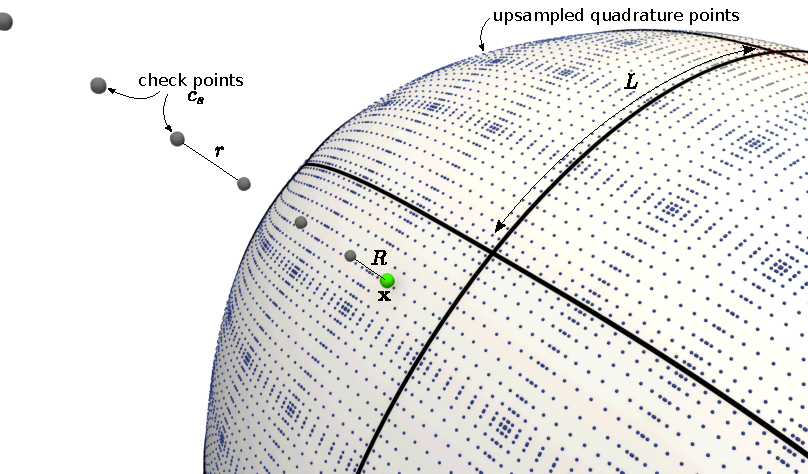
\includegraphics[width=.85\linewidth]{figs/qbkix_schematic.pdf}
  \end{minipage}\hfill
  \mcaption{fig:qbkix-schematic}{Schematic of singular/near-singular
  evaluation}{A small piece of a boundary $\Gammah$ is shown, along with the set of
  patches $\Pcoarse$ (patch boundaries are drawn in black). The target point $\vx$, in this
  case on $\Gammah$, is shown in green. The solution is evaluated
  at the check points $\vc_s$ (gray points off-surface) using the fine
  discretization $\Pfine$ (small dots on-surface). The distance from the first
  check point $\vc_0$ to $\Gammah$ is $R$ and the distance between consecutive
  check points $\vc_i$ and $\vc_{i+1}$ is $r$. In this example, $\Pfine$ is computed
  from $\Pcoarse$ with two levels of uniform quadrisection, producing 16 times
  more patches. The patch length $L$ is roughly proportional to the average edge
  length of the patch.}
\end{figure}

For the remaining points in $\Omega_N$, we need an alternative means of evaluating the solution.
In the spirit of the near-singular evaluation method of \cite{YBZ},  we construct a set of \textit{check points} $\vc_0, \hdots, \vc_p$ in $\Omega_I$ along a line intersecting $\vx$ to approximate the solution near $\vx$. 
However, instead of interpolating the solution as in \cite{YBZ}, we instead extrapolate the solution from the check points to $\vx$.
%We first place check points in $\Omega_I$, compute $\hat{u}(\vc_i, \Pfine)$ for each $i$, then extrapolate the approximate values at the check points to $\vx$.  \note[MJM]{kill sentence}
We define two distances relative to $\vsx$: $R(\vsx) =b L_\vsx = \|\vc_0 - \vsx\|_2$, the distance from the first check point $\vc_0$ to $\Gammah$,  and $r(\vsx) =a L_\vsx = \|\vc_i - \vc_{i+1}\|_2$, the distance between consecutive check points.
We assume  $0<a,b <1$.
%The points are placed along the surface normal $\vn(\vsx)$. 

The overall algorithm for the unified singular/near-singular evaluation scheme is as follows.
A schematic for \qbkix is depicted in \Cref{fig:qbkix-schematic}.


\begin{enumerate}
  \item Find the closest point $\vsx$ on $\Gammah$ to $\vx$.
  \item Given values $a$ and $b$, generate check points $C = \{\vc_0, \hdots, \vc_{p}\}$ 
    %distance $R(\vy)$ away from the $\Gamma$ and equispaced in $\vr(\vy)$ along the inward-pointing normal:
    \begin{equation}
      \vc_s = \vsx -(R(\vsx) +s r(\vsx)) \vn(\vsx), \quad s=0, \hdots, p
      \label{eq:check}
    \end{equation}
    The center of mass of these check points $\vhc$ is called the \textit{check center} for $\vx$.
    Note that $\Pfine$ must satisfy the condition that $\vc_s$ are in $\Omega_I$ for a given choice of $a$ and $b$.
\item Upsample $\phi$. 
  We interpolate the density values $\phi_I$ at $x_I$ on patches in $\Pcoarse$ to quadrature points $\tilde{x}_J$ on patches in $\Pfine$ 
  with global indices $I$ and $J$ on $\Pcoarse$ and $\Pfine$ respectively.
  If a patch $\vP_i$ in $\Pcoarse$ is split into $m_i$ patches in $\Pfine$, we are interpolating from $q^2$ points to $m_iq^2$ points.
  %Let $\wfine$ and $\phifine$ be the vector quadrature weights and interpolated density values at $\tilde{x}_J$ of $\Pfine$.
  \item Evaluate the potential at check points via smooth quadrature with the upsampled density, i.e. evaluate $\hat{u}(\vc_s) = \hat{u}(\vc_s, \Pfine)$ for $s=0,\hdots, p$.
  \item Compute a Lagrange interpolant $\tilde{u}$ through the check points $\vc_0,\hdots, \vc_p$ and values $\hat{u}(\vc_0), \hdots, \hat{u}(\vc_{p})$ and evaluate at the interpolant at $\vx$:
      \begin{equation}
          \tilde{u}(\vx) = \sum_{s=0}^p \hat{u}(\vc_s)\ell_s(t_\vx),
      \end{equation}
        where $\ell_s(\vx)$ is the $s$th Lagrange basis function through the points $\vc_0,\hdots, \vc_p$, and $t_\vx\in \mathbb{R}$ is such that $\vx = \vsx - t_\vx\vn(\vsx)$ (see \cref{fig:extrap-err-setup} for a schematic of the check points).
    Since $\vx$ lies between $\vc_0$ and $\Gammah$, we are extrapolating when computing $\tilde{u}(\vx)$.
\end{enumerate}

%\begin{algorithm}
%    \KwData{A set of surface patches $\Pcoarse$, a set of quadrature patches $\qPfine$, a target point $\vx$, extrapolation order $p$, quadrature order $q$, }
%  \KwResult{The closest point $\vsx$ on $\qP$ to $\vx$}
%
%  \DontPrintSemicolon
%  Construct an AABB tree $T_T$ from a fine triangle mesh of the quadrature patches of $\qP$\;
%  Construct an AABB tree $T_B$ from bounding boxes of quadrature patches in $\qP$.\;
%    $\tau_0 = $ closest triangle to $\vx$ computed with $T_T$ \;
%  
%    $P_{i_0} = $ patch corresponding to $\tau_0$\;
%    Find the closest point $\vector{s}_{\vector{\vx},0}$ on $P_{i_0}$ to $\vx$ with \cref{app:closest_point}.\;
%    $d_{i_0} = \|\vx - \vector{s}_{\vector{\vx},0}\|_2$\;
%    $B_{d_{i_0}}(\vx)=$ a box centered a $\vx$ with edge length $2d_{i_0}$\;
%    Find the boxes $B_{i_1}, \hdots B_{i_k}$ in $T_B$ that intersect $B_{d_{i_0}}(\vx)$\;
%    
%    \For{$B_{i_j} \in B_{i_1}, \hdots B_{i_k}$}{
%      $P_{i_j} =$ quadrature patch corresponding to $B_{i_j}$ \;
%      Find the closest point $\vector{s}_{\vector{\vx},j}$ on $P_{i_j}$ to $\vx$ with \cref{app:closest_point} to precision $\err{opt}$.\;
%      $d_{i_j} = \|\vx - \vector{s}_{\vector{\vx},j}\|_2$\;
%    }
%    $j^* = \mathrm{argmin}_j\{d_{i_j}\}$ \;
%    \Return{$\vector{s}_{\vector{x},j^*}$}
%  \mcaption{alg:singular_eval}{Evaluate the singular/near-singular layer potential at $\vx$}{}
%\end{algorithm}
%The parameters involved in this scheme are the number of check points $p$ and the relative spacing parameters of the check points $a$ and $b$.
%A critical aspect of the scheme is ensuring that the check points are in the intermediate field, i.e., $\Pfine$ is chosen to satisfy this condition.
%We use the error discussion in \cref{sec:error} and the algorithms of \cref{sec:adaptive_upsampling} to compute values of $a$, $b$ and  $\Pfine$ for a given $\etrg$.

\paragraph*{Ill-conditioning of the discrete integral operator}
%This scheme is used to compute singular integrals needed in the iterative solver for the solution of \cref{eq:int-eq}.
This evaluation scheme can be used directly to extrapolate all the way to the surface and obtain the
values of the singular integral in \cref{eq:int-eq}.
However, in practice, due to a distorted eigenspectrum of this approximate operator, \gmres tends to stagnate at a level of error corresponding to the accuracy of \qbkix when it is used to compute the matrix-vector product.
This is a well-known phenomenon of approximation-based singular quadrature schemes; \cite[Section 3.5]{KBGN}\cite[Section 4.2]{RBZ} present a more detailed study.
To address this, we average the interior and exterior limits of the solution at the quadrature nodes, computed via \qbkix, to compute the on-surface potential and add $\frac{1}{2}I$ to produce the interior limit.
This shifts the clustering of eigenvalues from around zero to around $\frac{1}{2}$, which is ideal from the perspective of \gmres.
We call this \textit{two-sided} \qbkix, while the standard version described above is called \textit{one-sided} \qbkix.
We observe stable and consistent convergence of \gmres when two-sided \qbkix is used to evaluate the matrix-vector multiply to solve \cref{eq:linear_system}. 
In light of this, we always use two-sided \qbkix within \gmres and set the stopping tolerance for \gmres to $\err{\gmres}=10^{-12}$, regardless of the geometry, boundary condition or  quadrature order. 

\subsection{Geometric criteria for accurate quadrature\label{sec:geom_criteria}}
The accuracy of the method outlined above is controlled by two competing error terms: \textit{quadrature error} incurred from approximating the layer potential \cref{eq:double_layer} with \cref{eq:double_layer_disc} in Step 4 and \textit{extrapolation error} due to approximating the singular integral with an extratpolated value in Step 5.
Both errors are determined by the location of check points relative to the patches in $\Pcoarse$ and $\Pfine$ (see \Cref{heuristic:error_quad_high_order,thm:extrap_error}). 

\begin{figure}[!htb]
  \centering
  %\setlength\figureheight{1.9in}
  %\setlength\figurewidth{2.1in}
  \begin{minipage}{.33\textwidth}
      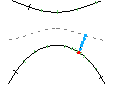
\includegraphics[width=\linewidth]{figs/admissibility_motivation2.pdf}
  \end{minipage}\hfill
  \begin{minipage}{.33\textwidth}
    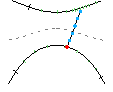
\includegraphics[width=\linewidth]{figs/admissibility_motivation1.pdf}
  \end{minipage}\hfill
  \begin{minipage}{.33\textwidth}
    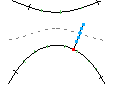
\includegraphics[width=\linewidth]{figs/admissibility_motivation3.pdf}
  \end{minipage}\hfill
  \mcaption{fig:admissibility-motivation}{Possible check point configurations}{A \twod  example depicting three choices of $a$ and $b$ in \cref{eq:check}. 
 Shown is the boundary $\Gammah$, with black tick marks denoting patch boundaries of $\Pcoarse$, green tick marks denoting patch boundaries of $\Pfine$, the target point (red dots), its check points (blue dots) along the normal closest to the target point, and the medial axis of $\Gammah$ (gray dotted line).
Large (left) and small (middle) values of $a$ and $b$ can cause clustering of check points near to $\Gammah$, which requires large amounts of upsampling to compute the potential accurately. Using the medial axis as a heuristic to for admissibility (right), we can minimize the amount of adaptive upsampling required.}
\end{figure}
In \Cref{fig:admissibility-motivation}, we show three examples of different choices of check point locations to evaluate the potential at a point with \qbkix. 
%Suppose that we have chosen extrapolation parameters $a$ and $b$ such that the extrapolation accuracy is less then $\etrg$, following the discussions in \cref{sec:extrap_error,sec:parameter-selection}. From an accuracy perspective, each choice of parameters is are equally valid. 
%However, each choice will require a different set $\Pfine$ in order to ensure accurate integration in \cref{eq:double_layer_disc}.
In \cref{fig:admissibility-motivation}-left, $\vc_0$ is placed close to the target point, while in \cref{fig:admissibility-motivation}-middle, $\vc_0$ is far from the target point, but $\vc_p$ is close to a non-local piece of $\Gammah$. 
Both cases will require excessive refinement of $\Pcoarse$ in order to resolve \cref{eq:double_layer_disc} accurately with $\Pfine$.
On the other hand, in \cref{fig:admissibility-motivation}-right, we can either perform one refinement step on $\Pcoarse$ or adjust $a$ and $b$, which will result in fewer patches in $\Pfine$, and therefore provide a faster integral evaluation, while maintaining accuracy.

In an attempt to strike this balance between speed and accuracy, we need certain constraints on the geometry of $\Gammah$ to ensure the efficient and accurate application of \qbkix, which we impose on the patch sets $\Pcoarse$ and $\Pfine$.
We will first outline our constraints on the quadrature patch sets $\Pcoarse$ and $\Pfine$ which allow for accurate evaluation with \qbkix.

\subsubsection{Admissibility criteria\label{sec:admissible}}
A set of patches $\qP$ is \textit{admissibile} if the following statements are satisfied on each quadrature patch in $\qP$:
\begin{criteria}
  \item The error of a surface patch $\vP_i$ approximating an embedding $\gamma_r$ is below some absolute target accuracy $\err{g}$ \label{criteria:1}
  \item The interpolation error of the boundary condition $f$ is below some absolute target accuracy $\err{f}$ \label{criteria:2}
  \item For each check center $\vhc_j$ corresponding to the quadrature point $\vy_j$ on the surface, the closest point on $\hat{\Gamma}$ to $\vhc_j$ is $\vy_j$. \label{criteria:3}
%  \item Each patch has characteristic length $L \geq L_\lbl{min}$.\label{criteria:4}
\end{criteria}

\Cref{criteria:1} is required to ensure that $\Gammah$ approximates $\Gamma$ with sufficient accuracy to solve the integral equation.
We discuss how to choose $\err{g}$ in \cite[Section 6]{morse2020bsupplementary}; for the tests in this paper, we simply choose $\err{g} < \err{target}$.
\Cref{criteria:2} guarantees that $f$ can be represented at least as accurately as the desired solution accuracy.
We therefore similarly choose $\err{f} < \etrg$. 
%The parameters $a$ and $b$ in \cref{eq:check} are chosen to place check points to balance the extrapolation error, which grows as $a$ and $b$ increase, and smooth quadrature error, which grows as $a$ and $b$ decrease, while attempting to minimize cost.
\Cref{criteria:3}  balances the competing geometric constraints of cost and accuracy by flexibly placing check points as far as possible from $\Gammah$ without causing too much upsampling on other patches.
%Rather than checking all check point locations individually, we use the check center $\vhc$ as a proxy.
If a check point $\vc$ constructed from a surface patch $\vP$ is too close to another surface patch $\vP'$, \Cref{criteria:3} will indicate that $\vP$ is inadmissible. 
If $\vP$ is subdivided into its children, new check points $\vc^\prime$ generated from these children of $\vP$ will be closer to $\vP$ and further from $\vP'$.
Since check points are placed at distances proportional to $L(\vP)$, repeated refinement of $\vP$ will eventually satisfy \Cref{criteria:3}. 

\subsubsection{Upsampling criteria\label{sec:adaptive_upsampling}}
Once we have a set of admissible surface patches satisfying \Cref{criteria:1,criteria:2,criteria:3}, we need to determine the upsampled quadrature patches $\Pfine$ that ensure that the check points generated from $\Pcoarse$ are in $\Omega_I$, i.e., $\|u(\vc) - \hat{u}(\vc, \Pfine)\| < \etrg$.
%Once the set of admissible surface patches $\Pcoarse$ is computed, we need to determine the upsampled quadrature patches $\Pfine$ that ensure that the check points generated from $\Pcoarse$ are in $\Omega_I$, i.e., $\|u(\vc) - \hat{u}(\vc, \Pfine)\| < \etrg$.
To achieve this, we need a criterion to determine which patches are ``too close'' to a given check point for the error to be below $\err{target}$.
We make the following assumption about the accuracy of our smooth quadrature rule: \textit{\cref{eq:double_layer_disc} is accurate to $\err{target}$ at points further than  $L(\vP)$ from $\vP$, for $\err{target} > 10^{-12}$}.
This is motivated by \cite{aT2,barnett2014evaluation}, which demonstrate the rapid convergence of the layer potential quadrature error with respect to $\|\vx - \vsx\|_2$.  
For sufficiently high quadrature orders, such as $q=20$, this assumption seems to hold in practice.
We say that a point $\vx$ is \textit{near} to $\vP$ if the distance from $\vx$ to $\vP$ is less than $L(\vP)$; otherwise, $\vx$ is \textit{far} from $\vP$.
We would like all check points required for the singular/near-singular evaluation of the discretization of \cref{eq:double_layer} using \qbkix to be far from all patches in $\Pfine$.
If this is satisfied, then we know that the Clenshaw-Curtis quadrature rule will be accurate to $10^{-12}$ at each check point.

\subsection{Refinement algorithm preliminaries}
Computing the distance from a check point to a given patch is a fundamental step in verifying the constraints on $\Pcoarse$ and $\Pfine$ from \cref{sec:admissible,sec:adaptive_upsampling}. 
Before detailing our refinement algorithms to enforce these criteria, we introduce several geometric algorithms and data structures that will be used to compute the closest point on piecewise polynomial surfaces.

\subsubsection{\aabb trees\label{sec:aabb_trees}} 
In order to implement our algorithms to enforce admissibility efficiently, we use a fast spatial data structure to find the patches that are close to a query point $\vx$.
In \cite{RKO, wala20193d}, the quadtree and octree within an \fmm is extended to support the geometric queries needed for a fast \qbx  algorithm.
In this work, we use an axis-aligned bounding box (\aabb) tree, which is a type of bounding volume hierarchy \cite{samet2006foundations}, implemented in \texttt{geogram} \cite{geogram}.
An \aabb is a tree with nodes corresponding to bounding boxes and leaves corresponding to bounding boxes containing single objects. 
A bounding box $B_0$ is a child of another box $B_1$ if $B_0 \subset B_1$; the root node is a bounding box of the entire domain of interest.
Operations supported by \aabb trees include: (i) finding all bounding boxes containing a query point, (ii) finding all bounding boxes that intersect another query box, (iii) finding the closest triangle to a query point (because triangles have trivial bounding boxes). 
By decoupling geometric queries from fast summation, the individual algorithms can be more thoroughly optimized, in exchange for the additional memory overhead of maintaining two distinct data structures.
The query algorithm presented in \cite{lu2019scalable} likely has better parallel scalability, but \aabb trees are faster for small to medium problem sizes on a single machine due to less redundant computation.

To define an \aabb tree for our patch-based surface $\Gammah$, we make use of the following fact: the control points of a B\'ezier surface ($\vector{a}_{\ell m}$'s from \cref{eq:tensor-product}) form a convex hull around the surface that they define \cite{F}.
As a result, we can compute a bounding box of a surface or quadrature patch $\vP$ directly from the B\'ezier coefficients simply by computing the maximum and minimum values of each component of the $\vector{a}_{\ell m}$'s, as shown in \cref{fig:patch-coeffs-bbox}-middle.
This bounding box can then be inserted into the \aabb tree as a proxy for a surface or quadrature patch.
\begin{figure}[!htb]
  \centering
  %\setlength\figureheight{1.9in}
  %\setlength\figurewidth{2.1in}
  \begin{minipage}{.33\textwidth}
      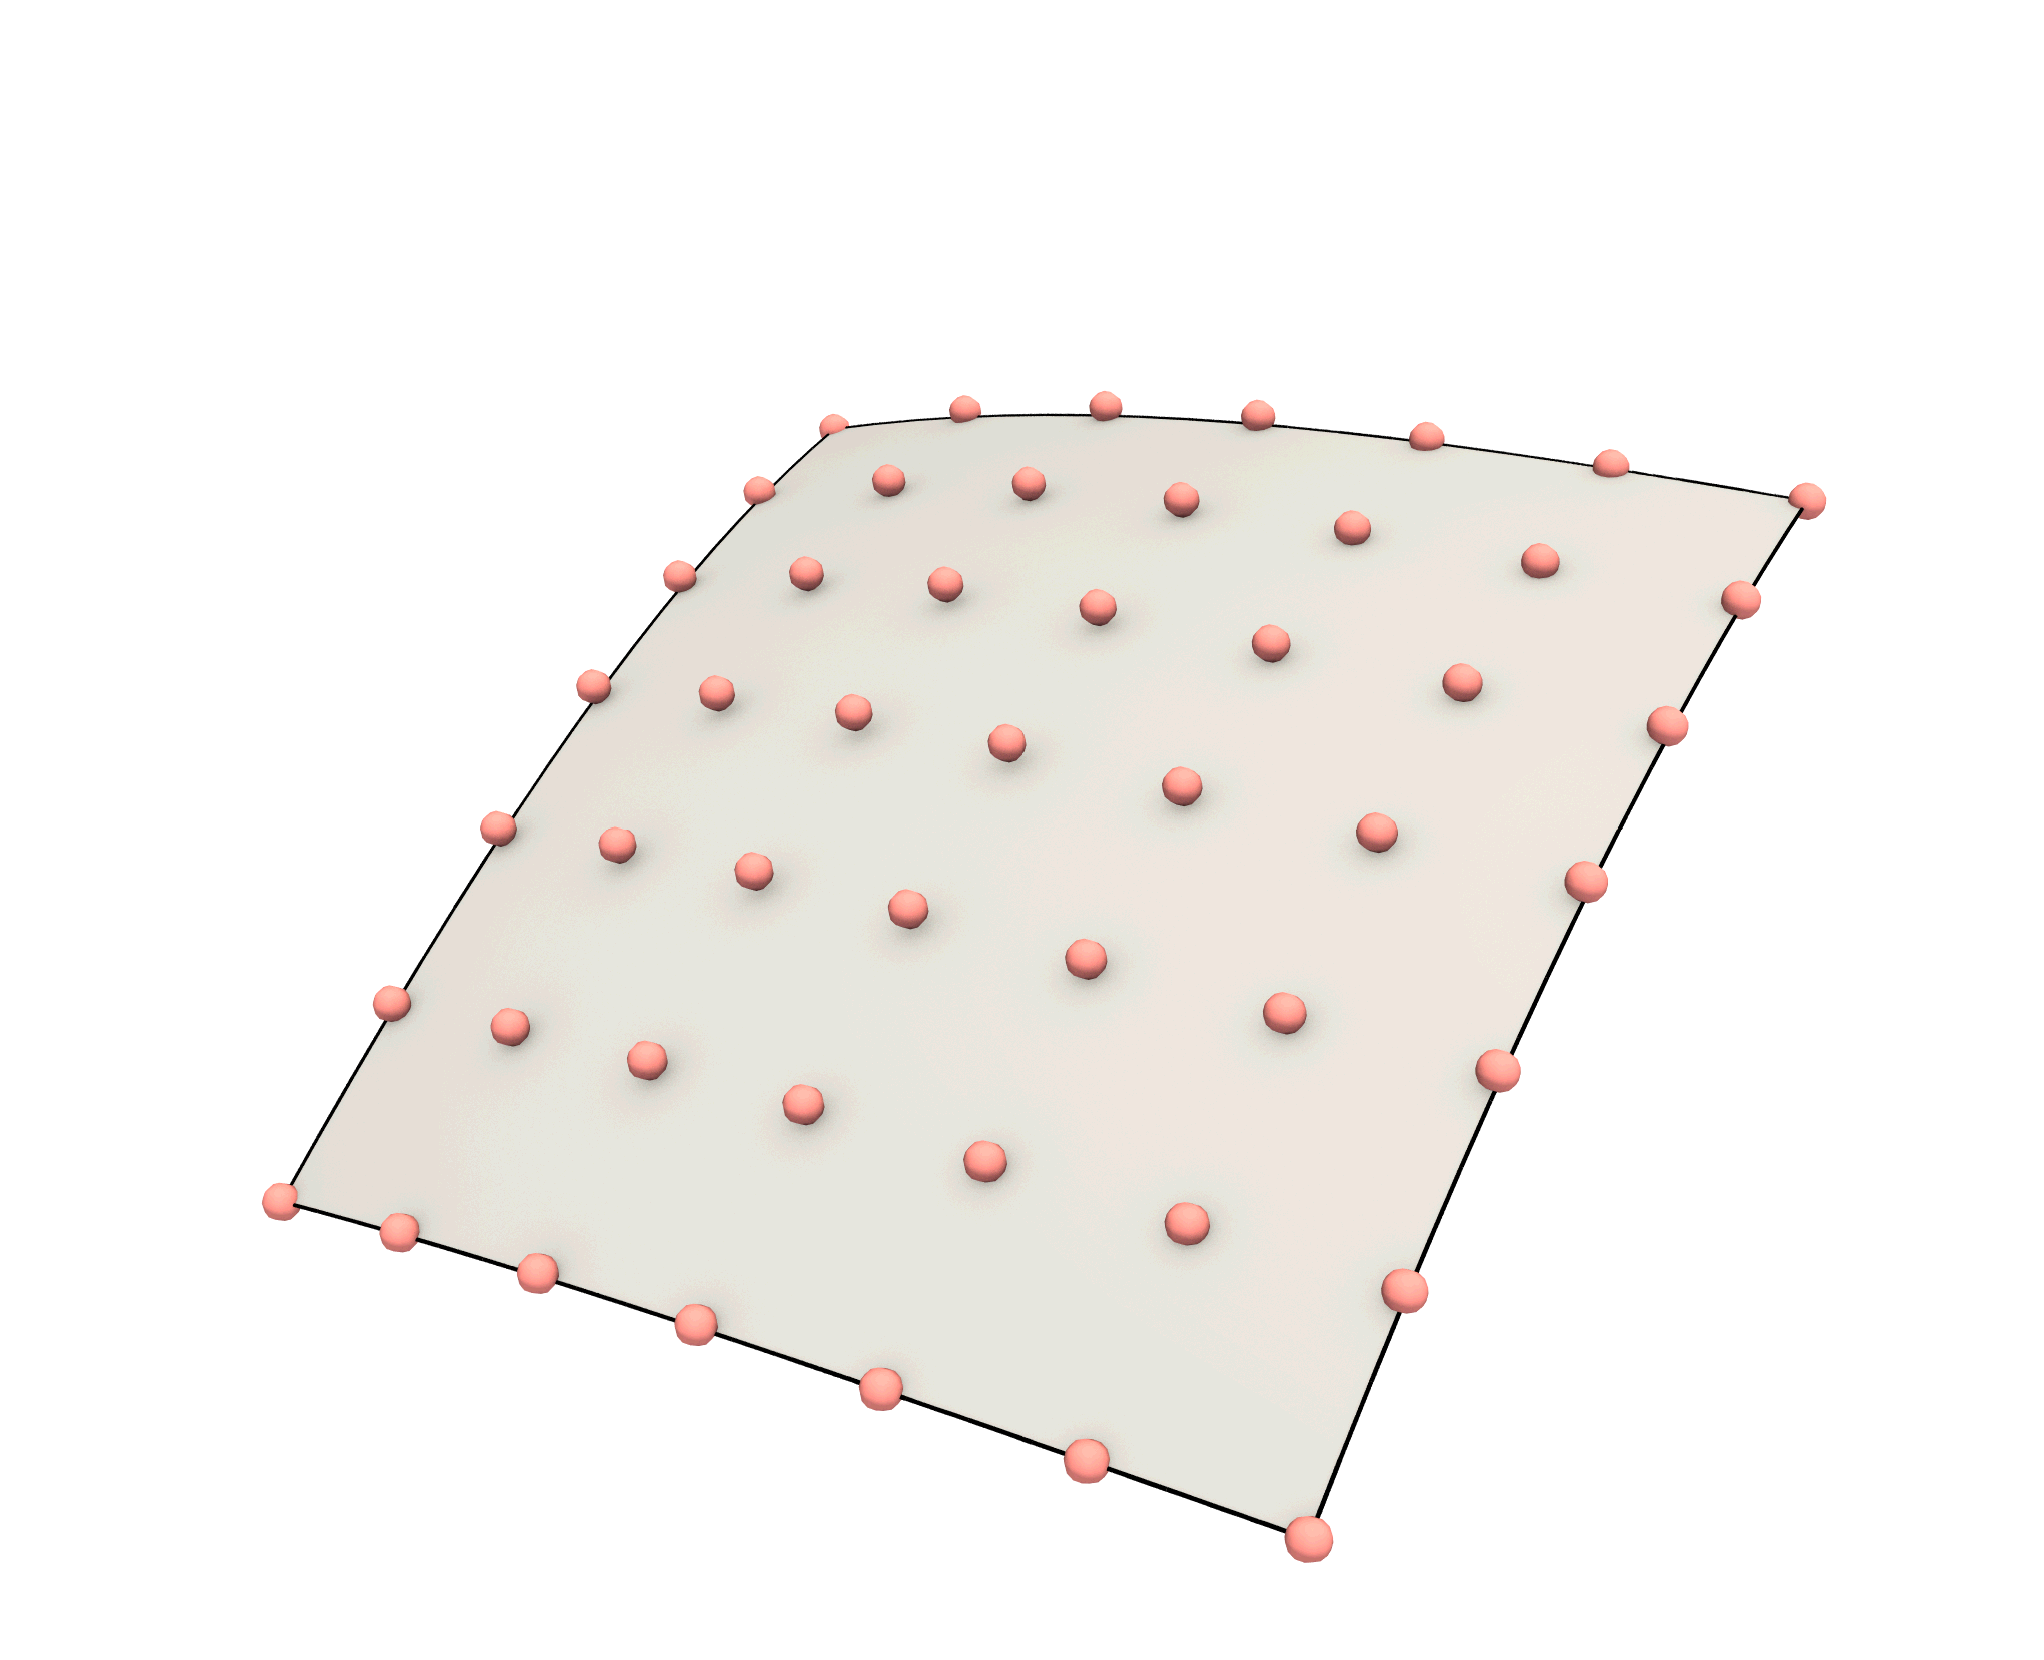
\includegraphics[width=\linewidth]{figs/patch_with_coeffs.png}
  \end{minipage}\hfill
  \begin{minipage}{.33\textwidth}
    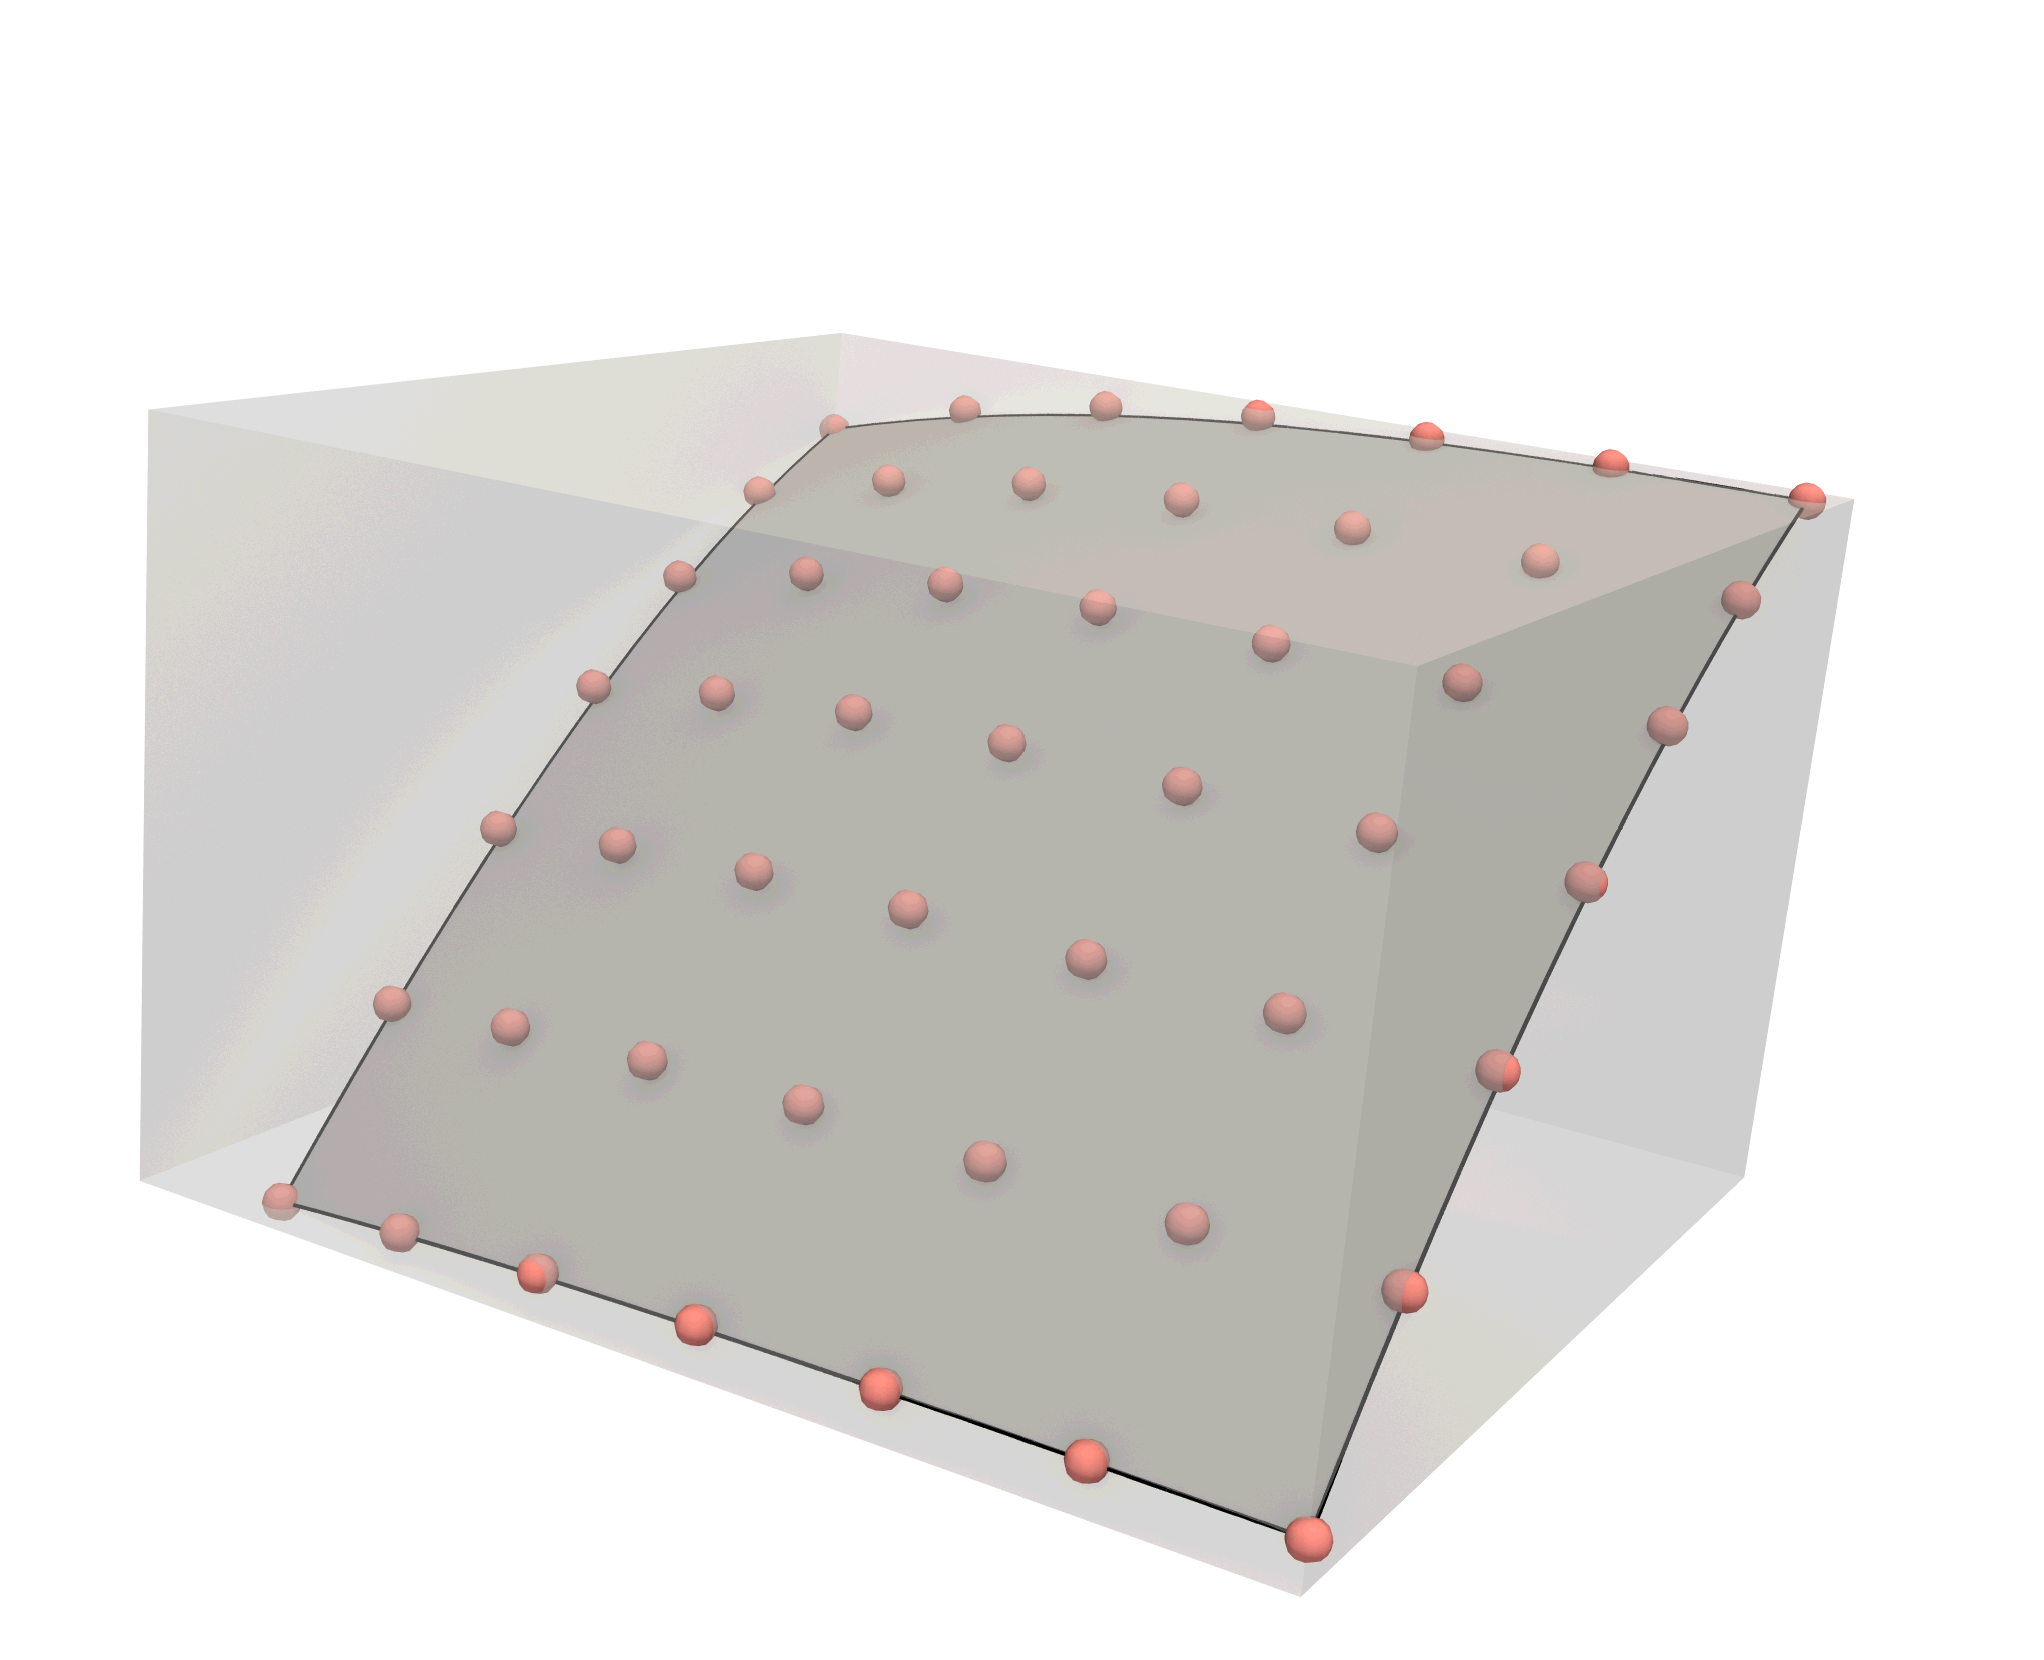
\includegraphics[width=\linewidth]{figs/patch_with_coeffs_bbox.png}
  \end{minipage}\hfill
  \begin{minipage}{.33\textwidth}
    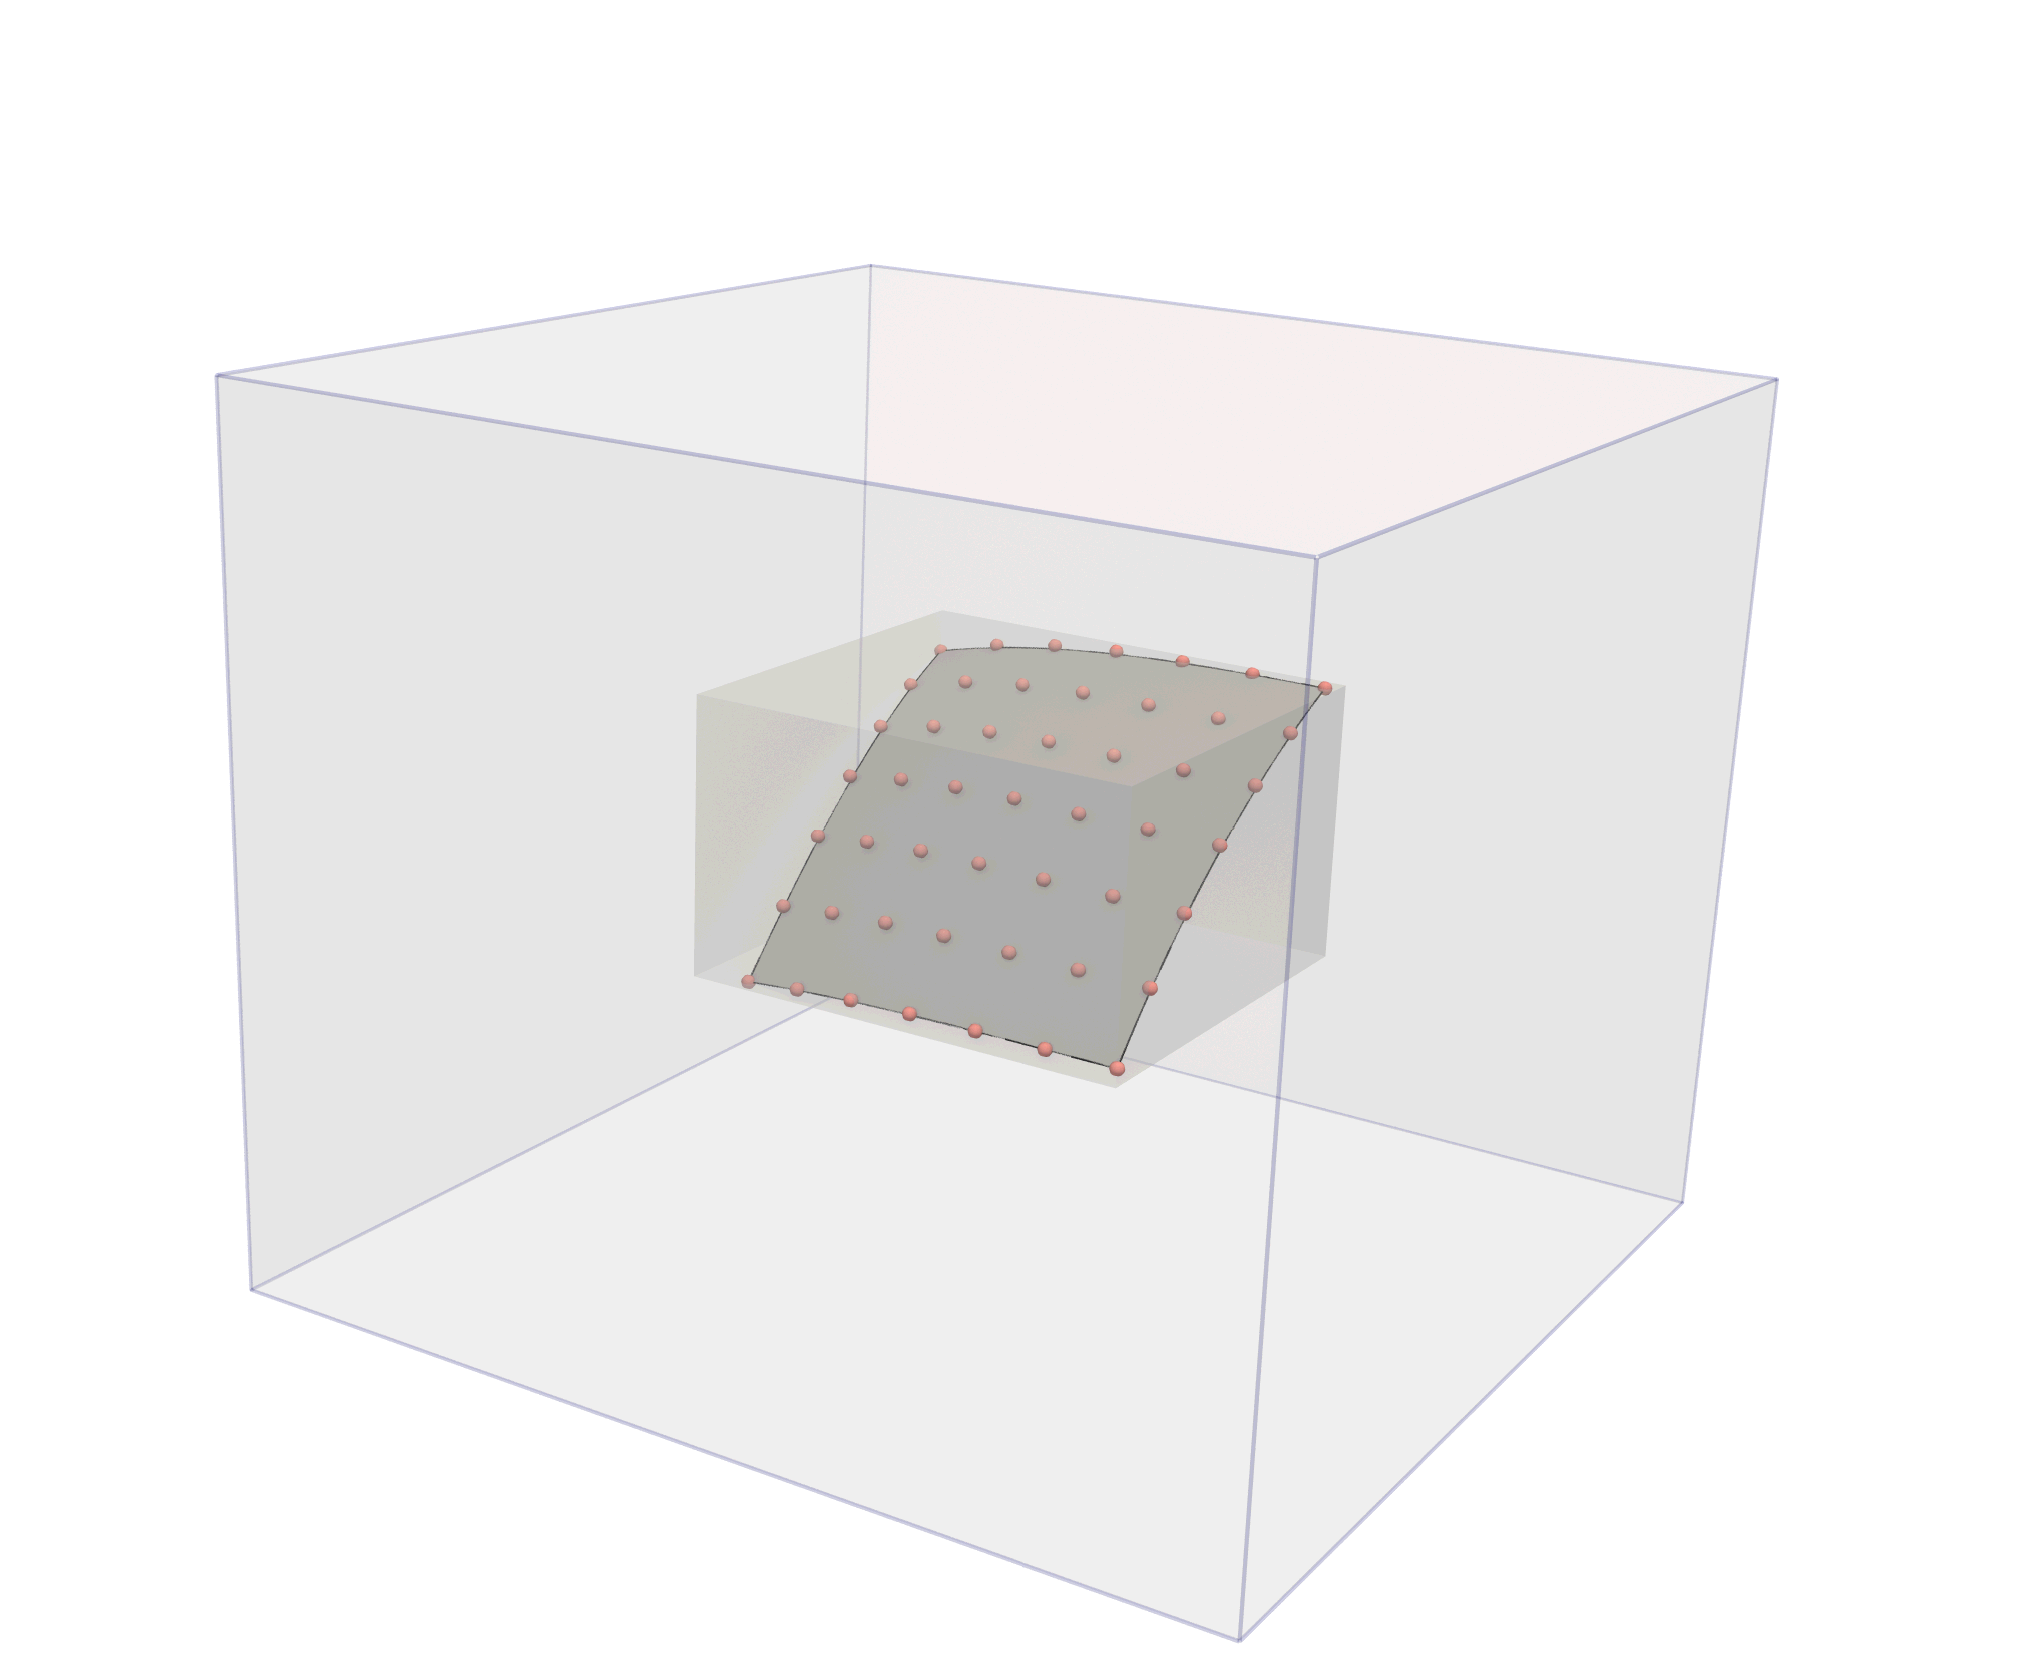
\includegraphics[width=\linewidth]{figs/patch_with_coeffs_near_bbox.png}
  \end{minipage}\hfill
  \mcaption{fig:patch-coeffs-bbox}{Relationship between control points and
  bounding boxes}{Left: a patch in the tensor product B\'ezier basis, with control
      points ($\vector{a}_{\ell m}$'s from \cref{eq:tensor-product}) plotted. The convex hull of the control points of a patch are guaranteed
      to contain the patch. Center: The patch bounding box, computed from the control
      points. Right: The near-zone bounding box of the patch from
      \cref{sec:adaptive_upsampling_algo} computed by
      inflating the bounding box by $L(\vP)$.
}
\end{figure}



\subsubsection{Computing the closest point to a patch\label{sec:closest_point_algo}}

To find a candidate closest patch $\vP_{i_0}$ to $\vx$, we construct a fine triangle mesh and bounding boxes of each patch in $\Pcoarse$ and insert them into an \aabb tree.
We can query the \aabb tree for the nearest triangle to $\vx$ with the \aabb tree, which corresponds to $\vP_{i_0}$.
We then compute the accurate true distance $d_{i_0}$ to $\vP_{i_0}$ using a constrained Newton method, presented in detail in \cref{app:closest_point}.

However, there may be other patches whose distance to $\vx$ is less than $d_{i_0}$, as shown in \cref{fig:candidate-near-patch}.
To handle this case, we then query the \aabb tree for all patches $\vP_{i_1}, \hdots, \vP_{i_k}$ that are distance at most $d_{i_0}$ from $\vx$.
This is achieved by forming a query box centered at $\vx$ with edge length $2d_{i_0}$ and querying the \aabb tree for all intersection bounding boxes. 
The precise distance is then computed for each patch  $\vP_{i_1}, \hdots, \vP_{i_k}$ with \cref{app:closest_point} and the smallest distance is chosen.
We summarize this process in \cref{alg:closest_point}.


\begin{algorithm}[!htp]
    \KwData{A set of quadrature patches $\qP$, a query point $\vx$, Newton method tolerance $\err{opt}$}
  \KwResult{The closest point $\vsx$ on $\qP$ to $\vx$}

  \DontPrintSemicolon
  Construct an AABB tree $T_T$ from a fine triangle mesh of the quadrature patches of $\qP$\;
  Construct an AABB tree $T_B$ from bounding boxes of quadrature patches in $\qP$.\;
    $\tau_0 = $ closest triangle to $\vx$ computed with $T_T$ \;
  
    $\vP_{i_0} = $ patch corresponding to $\tau_0$\;
    Find the closest point $\vector{s}_{\vector{\vx},0}$ on $\vP_{i_0}$ to $\vx$ with \cite[Section 2]{morse2020bsupplementary}.\;
    $d_{i_0} = \|\vx - \vector{s}_{\vector{\vx},0}\|_2$\;
    $B_{d_{i_0}}(\vx)=$ a box centered a $\vx$ with edge length $2d_{i_0}$\;
    Find the boxes $B_{i_1}, \hdots B_{i_k}$ in $T_B$ that intersect $B_{d_{i_0}}(\vx)$\;
    
    \For{$B_{i_j} \in B_{i_1}, \hdots B_{i_k}$}{
      $\vP_{i_j} =$ quadrature patch corresponding to $B_{i_j}$ \;
      Find the closest point $\vector{s}_{\vector{\vx},j}$ on $\vP_{i_j}$ to $\vx$ with \cite[Section 2]{morse2020bsupplementary} to precision $\err{opt}$.\;
      $d_{i_j} = \|\vx - \vector{s}_{\vector{\vx},j}\|_2$\;
    }
    $j^* = \mathrm{argmin}_j\{d_{i_j}\}$ \;
    \Return{$\vector{s}_{\vector{x},j^*}$}
  \mcaption{alg:closest_point}{Compute the closest point to $\vx$}{}
\end{algorithm}

\begin{figure}[!htb]
  \centering
  %\setlength\figureheight{1.9in}
  %\setlength\figurewidth{2.1in}
  \hfill
  \begin{minipage}{.3\textwidth}
      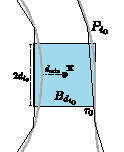
\includegraphics[width=\linewidth]{figs/candidate_near_patch_trimesh.pdf}
  \end{minipage}\hfill
  \mcaption{fig:candidate-near-patch}{A \twod schematic of near-patch candidate selection}{
      A visual depiction of the quantities defined in lines 3-7 of \cref{alg:closest_point} (shown here in \twod for simplicity), with notation matching \cref{alg:point_marking}.
      The triangle-mesh proxy is drawn in as black lines and patches are drawn as gray curves.
      We have found an initial closest triangle $\tau_0$ to $\vx$ corresponding to patch $\vP_{i_0}$ and computed $d(\vx, \vP_{i_0}) = d_{i_0}$.
      We then query the \aabb tree for all patches that intersect box $B_{d_{i_0}}$ with edge length $2d_{i_0}$, shown in blue.
      There is clearly a patch that is closer to $\vx$ than $\vP_{i_0}$ that will be returned from the query, which will be distance $d_\lbl{min}$ from $\vx$.
}
\end{figure}

\subsection{Admissibility algorithm\label{sec:admissible_algo}}
Our algorithm to enforce \cref{criteria:1,criteria:2,criteria:3} proceeds as follows:
\begin{itemize}
    \item To enforce \Cref{criteria:1}, we adaptively fit a set of surface patches to the embeddings $\gamma_r$ representing $\Gamma$.
We construct a bidegree $(n,n)$ piecewise polynomial least-squares approximation $\vP_i$ in the form of \cref{eq:tensor-product} to $\gamma_r$ on $I^2$.
        If $\vP_i$'s domain $\mathcal{D}_i$ is obtained by refinement of $E_r$, we fit $\vP_i \circ \eta_i$ to $\gamma_r$ on $\I^2$, using $4n \times 4n$ samples on $\I^2$. 
        If the pointwise error of $\vP_i$ and its partial derivatives is greater than $\err{g}$, then it is quadrisected and the process is repeated. 

\item  Once the embeddings are resolved, we resolve $f$ on each surface patch produced from the previous step in a similar fashion to enforce \Cref{criteria:2}.
  However, rather than a least-squares approximation in this stage, we use piecewise polynomial interpolation.
 
\item To enforce \Cref{criteria:3}, we construct the set of check centers $\vhc_I$ which correspond to the check points required to evaluate the solution at the quadrature nodes $\vy_I$.
    For each check center $\vhc_I$, we find the closest point $\vector{s}_{\vhc_I} \in \Gammah$.
    If $ \|\vector{s}_{\vhc_I} - \vy_I\| \geq \err{opt}$, we split the quadrature patch $\vP$ containing $\vy_I$.
        The tolerance $\err{opt}$ is used in the Newton's method in \cite[Section 2]{morse2020bsupplementary}; we usually choose $\err{opt}=10^{-14}$.
Since $d(\vhc_I,\Gammah)$ is proportional to $L_{\vy_I}$, the new centers $\vhc_I$ for the refined patches  will be closer to the surface. 
    We use \cref{alg:closest_point} to compute $\vector{s}_{\vhc_I}$.
        However, in the case of check points, we can skip lines 1-6 to compute $d_{i_0}$,  since $\vhc_I$ is $R + r(p+1)/2$ away from $\vy_I \in \vP(D)$ by construction.
        We can apply lines 7-14 of \cref{alg:closest_point} with $d_{i_0} = R + r(p+1)/2$ to compute $\vector{s}_{\vhc_I}$.
\end{itemize}

We summarize the algorithm to enforce \Cref{criteria:3} in \cref{alg:admissibility}.
At each refinement iteration, the offending patches are decreased by quadrisection, which reduces the distance from the quadrature point $\vy_I$ to its checkpoints.
This eventually satisfies \Cref{criteria:3} and the algorithm terminates. 

\begin{algorithm}[!ht]
  \KwData{A set of quadrature patches $\qP$, optimization tolerance $\err{opt}$}
  \KwResult{An admissible set of quadrature patches $\qP$}

  \DontPrintSemicolon
  $\qP = \Pcoarse$\;
  Mark all patches in $\qP$ as inadmissible.\;
  
  \While{any patch in $\qP$ is inadmissible}{
    Construct an AABB tree $T$ as described in \cref{sec:closest_point_algo} from $\qP$\;
    \For{$\vP \in \qP$}{
        \If{$\vP$ is inadmissible}{
            Construct a set of check centers $C_\vP$ for each $\vy_J \in \vP(D)$ \;

            \For{$\vhc \in C_\vP$}{
                $d_{i_0} = R + r(p+1)/2$\;
                Compute $\vector{s}_\vhc$ with lines 7-14 of \cref{alg:closest_point} with precision $\err{opt}$ and $d_{i_0}$.\;
                %Construct a box $B(\vhc)$ with edge length $2R + r(p+1)$ centered at $\vhc$.\;
                %$B_{i_1}, \hdots B_{i_k}$ = \texttt{query\_bbox\_intersections}($T$, $B(\vhc)$\texttt)\;
                %$P_{i_1}, \hdots P_{i_k}$ =  patches corresponding to $B_{i_1}, \hdots B_{i_k}$\;
                %\eIf{$P \in \{P_{i_1}, \hdots P_{i_k}\}$}{
                %    Compute candidate closest points $\vector{s}_\vhc^{(1)}, \hdots \vector{s}_\vhc^{(k)}$ on $P_{i_1}, \hdots P_{i_k}$ to $\vhc$ with \cref{app:closest_point} to accuracy $\err{opt}.$\;
                %    $\vector{s}_\vhc = \mathrm{argmin}_i \|\vector{s}_\vhc^{(i)}, - \vhc\|_2$\;
                \eIf{$\|\vector{s}_\vhc -\vy_J\|_2 < \err{opt}$}{
                    Mark $\vP$ as admissible.\;
                } {
                    Mark $\vP$ as inadmissible.\;
                    break   \tcp{only need one bad check center to mark $\vP$ for refinement}
                }
            }
        }
    }
    \For{$\vP \in \qP$}{
      \If{$\vP$ is inadmissible}{
        Split $\vP$ into its four child patches, mark each as inadmissible, and replace $\vP$ with its children in $\qP$.
      }
    }
  }
  \Return{$\qP$}
  \mcaption{alg:admissibility}{Enforce admissibility \Cref{criteria:3} on a set of quadrature patches}{}
\end{algorithm}

\subsection{Adaptive upsampling algorithm \label{sec:adaptive_upsampling_algo}}
%Simply applying the point marking algorithm detailed \cref{app:point_marking} to each check point is not sufficient.
Before detailing our upsampling algorithm to satisfy the criteria outlined in \cref{sec:adaptive_upsampling}, we must define the notion of a \textit{near-zone bounding box} of a quadrature patch $\vP$, denoted $B_\lbl{near}(\vP)$.
The near-zone bounding box of $\vP$ is computed as described in \cref{sec:aabb_trees}, but then is inflated by $2L(\vP)$, as shown in \cref{fig:patch-coeffs-bbox}-right.
This inflation guarantees that any point $\vx$ that is near $\vP$ is contained in $B_\lbl{near}(\vP)$ and, for an admissible set of quadrature patches $\Pcoarse$, that any $\vx\in \Omega_N$ must be contained in some quadrature patch's near-zone bounding box.
This means that by forming $B_\lbl{near}(\vP)$ for each quadrature patch in $\Pfine$, a check point is in $\Omega_I$ if it is not contained in any near-zone bounding boxes.

To compute the upsampled patch set from $\Pcoarse$, we initially set $\Pfine = \Pcoarse$, compute the near-zone bounding boxes of each patch in $\Pfine$ and insert them into an \aabb tree.
We also construct the set of check points $C$ required to evaluate our discretized layer-potential with \qbkix (\cref{sec:singular-eval}).
For each check point $\vc \in C$, we query the \aabb tree for all near-zone bounding boxes that contain $\vc$.
If there are no such boxes, we know $\vc$ is far from all quadrature patches and can continue.
If, however, there are near-zone bounding boxes $B_{i_0},\hdots, B_{i_k}$ containing $\vc$, we compute the distances $d_{i_k}$ from $\vc$ to $\vP_{i_1},\hdots,\vP_{i_k}$ using \cref{app:closest_point}.
If $d_{i_k} < L(\vP_{i_k})$, we replace $\vP_{i_k}$ in $\Pfine$ with its four children produced by quadrisection.


To improve the performance of this refinement procedure, we allow for the option to skip the Newton method in \cref{alg:closest_point} and immediately refine all patches $\vP_{i_0},\hdots \vP_{i_k}$.
This is advantageous in the early iterations of the algorithm, when most check points are near to patches by design.
We allow for a parameter $n_\lbl{skip}$ to indicate the number of iterations to skip the Newton optimization and trigger refinement immediately.
We typically set $n_\lbl{skip}=2$.
We summarize our algorithm in \cref{alg:adaptive_upsampling}.
%We first use the error estimate of \cref{sec:quad_error_heuristic} to determine the distance from the intermediate field $\Omega_I$ to the patch $P$,  which we will call $d_\lbl{near}(P)$.
%We compute a bounding box of $P$ as described in \cref{sec:mark_near}.
%We compute a bounding box of each patch $P$ in $\Pfine$ as described in \cref{sec:aabb_trees}.
%We then inflate the box size by $2d_\lbl{near}$ to produce the \textit{near-zone bounding box} of $P$, denoted $B_\lbl{near}(P)$, as shown in \cref{fig:patch-coeffs-bbox}-right. 
%We then inflate the each boxes' size by $2L(P)$ to produce the \textit{near-zone bounding box} of $P$, denoted $B_\lbl{near}(P)$, as shown in \cref{fig:patch-coeffs-bbox}-right. 

%However, we need to still determine if a point $\vc$ in $B_\lbl{near}(P)$ is actually near to $P$, which requires computing the distance from $\vc$ to $\Gammah$.

%To check this efficiently, we insert all the near-zone bounding boxes into an \aabb tree. 
%Let $C$ be the set of all check points required to evaluate our discretized layer potential.
%For each check point $\vc \in C$, we query the tree for all boxes containing $\vc$.
%The set of quadrature patches corresponding to the returned set of boxes are candidate patches for upsampling.
%We can now check the distance from $\vc$ to each of these quadrature patches using \cref{app:closest_point} and trigger refinement if the distance between $\vc$ and a given patch is less than $L$.
%Alternatively, one can also simply trigger refinement on all of the patches returned by the \aabb tree query without explicitly checking the distance.
%This is a cheaper operation that avoids the Newton iterations of \cref{app:closest_point}, but is less accurate and can cause over-refinement.
%One can either trigger upsampling on all of these patches or explicitly compute the distance from $\vc$ to each quadrature patch using .
%The former is a cheaper condition to check but less accurate; the latter is more precise and triggers less upsampling overall, but more expensive.
%This bounding box proxy is an over-approximation of $\Omega_N$; there are many cases in which a check point is contained in a near-zone bounding box, but strictly in $\Omega_I$.
%In these cases, the true distance from $\vc$ to each quadrature patch is more accurate.
%We strike a balance by triggering upsampling for all returned quadrature patches for the first iteration or two of upsampling and explicitly check distance to patches for the remaining iterations.

%The set $C$ is determined by $\Pcoarse$ and therefore fixed. 
%The average size of near-zone bounding boxes decreases after each step of refinement until the algorithm terminates; eventually no near-zone bounding boxes will contain check points.
%We summarize in \cref{alg:adaptive_upsampling}.

\begin{algorithm}[!htp]
    \KwData{An admissible patch set $\qP$, number of iterations $n_\lbl{skip}$ before using \cite[Section 2]{morse2020bsupplementary}}
  \KwResult{An upsampled set of quadrature patches}
  
  \DontPrintSemicolon
  Compute inflated near-zone bounding boxes $B_1, \hdots,  B_N$ of each $\vP \in \qP$.\;
  Construct an AABB tree $T$ from the near-zone bounding boxes.\;
  Construct all check points $C$ required to evaluate the \cref{eq:int-eq} on $\qP$.\;

  $\qP_\lbl{fine} = \qP$\;
  Mark all check points in $C$ as near.\;
  $i=0$

  \While{any $\vc \in C$ is marked near}{
    \For{$\vc \in C$}{
        \If{$\vc$ is marked near}{
            Query $T$ for all bounding boxes $B_{i_1}, \hdots B_{i_k}$ containing $\vc$.\;
            $\vP_{i_1}, \hdots \vP_{i_k} = $ patches corresponding to boxes $B_{i_1}, \hdots B_{i_k}$\;
            Mark $\vc$ as far\;
            \For{$\vP \in \vP_{i_1}, \hdots \vP_{i_k}$}{
                \eIf{$i > n_\lbl{skip}$}{
                    Find the closest point $\vector{s}_{\vc}$ on $\vP$ to $\vc$ with \cref{alg:closest_point}.\;
                    %\If{The error estimate in \cref{sec:quad_error_heuristic} is greater than $\eps$ with $d = \|\vy - \vc\|_2$}{
                    \If{ $\|\vector{s}_{\vc} - \vc\|_2 < L(\vP)$}{
                        Split $\vP$ and replace it in $\qP_\lbl{fine}$ with its children. \;
                        Mark $\vc$ as near\;
                    }
                } {
                    Split $\vP$ and replace it in $\qP_\lbl{fine}$ with its children.\;
                    Mark $\vc$ as near\;
                }
 
            }
       }
    }
    $i=i+1$\;

  }
    \mcaption{alg:adaptive_upsampling}{Adaptively upsample to accurately evaluate \cref{eq:double_layer_disc} at check points}{}
\end{algorithm}

%In \cite{RKO}, the panel size of the quadrature rule was tied to the distance of the \qbx expansion center from the boundary.
%This design choice produces an artificial dependence of the quadrature and expansion error, since the global upsampling factor for the fine discretization is determined by the closest expansion to the boundary.
%\cite{wala20193d} first presented an approach that decouples the coarse and fine discretizations; we follow a similar approach here.
%However, their approach does not explicitly depend on surface curvature, which has a dramatic impact on quadrature accuracy, which can lead to unnecessary upsampling.
%By taking advantage of the error heuristic in \cref{sec:error}, we are able to accurately determine quadrature accuracy at a given check point.

\subsection{Marking target points for evaluation\label{app:point_marking}}

Once we have solved \cref{eq:linear_system} for $\phi$ on $\Gammah$, we need the ability to evaluate \cref{eq:double_layer} at an arbitrary set of points in the domain.
For a target point $\vx$, in order apply the algorithm in \cref{sec:singular-eval}, we need to determine whether or not $\vx \in \Omega$ and, if so, whether $\vx $ is in $\Omega_N, \Omega_I$ or $\Omega_F$.
Both of these questions can be answered by computing the closest point $\vsx$ on $\Gammah$ to $\vx$. % with \cref{app:closest_point_opt}.
If $\vn(\vsx)\cdot(\vx - \vsx) < 0$, then $\vx \in \Omega$. 
As we have seen in \cref{sec:adaptive_upsampling}, the distance $\|\vx - \vsx\|$ determines whether $\vx \in \Omega_N,\Omega_I$ or $\Omega_F$.
However, for large numbers of target points, a brute force calculation of closest points on $\Gammah$ to all target points is prohibitively expensive.
We present an accelerated algorithm combining \cref{alg:closest_point} and an \fmm evaluation to require only constant work per target point. 


\subsubsection{Marking and culling far points \label{sec:mark_far}}
A severe shortcoming of \cref{alg:closest_point} is that its performance deteriorates as the distance from $\vx$ to $\Gammah$ increases. 
Consider the case where $\Gammah$ is a sphere with radius $r$ with $\vx$ at its center.
The first stage of \cref{alg:closest_point} returns a single quadrature patch that is distance $r$ from $\vx$; the next stage will return all quadrature patches.
This will take $O(N)$ time to check the distance to each patch.
Even on more typical geometries, we observe poor performance of \cref{alg:closest_point} when $\vx$ is far from $\Gammah$.

%It's important that we can mark points in $\Omega_F$ and mark points as inside or outside $\Omega$ without using \cref{sec:mark_near}.
To address this, we use an additional \fmm-based acceleration step to mark most points far from $\Gammah$ before using applying \cref{alg:closest_point}. 
Our approach is based on computing the generalized winding number \cite{jacobson2013robust} of $\Gammah$ at the evaluation points. 
For closed curves in $\mathbb{R}^2$, the \textit{winding number} at a point counts the number of times the curve travels around that point. 
The \textit{generalized winding number} of a surface $\Gammah$ at a point $\vx \in \mathbb{R}^3$ can be written as 
%\begin{equation}
%\omega_{\Gammah}(\vx) = %\frac{1}{4\pi} W_S(\vx) =
%  \frac{1}{4\pi}\iint_{\Gammah} sin(\phi)d\phi d\theta, \quad (\text{when }\vx =0).
%  \label{eq:gen_winding}
%\end{equation}
%%where $W(\vx)$ is the solid angle subtended by $S$. 
%%This is the projection of $S$ onto the unit sphere centered at $\vx$.
%The integrand can be interpreted as the signed differential solid angle subtended by an infinitesimal surface patch centered at $\vx$.
%
%In our case, $\Gammah$ is composed of a collection of surface patches with independent parametrizations, and can be computed patch by patch.
%%It's clear that the solid angle of $\Gammah$ with respect to $\vx$ is the sum of the solid angles of the surface patches:
%\begin{equation}
%  \omega_{\Gammah}(\vx) = \frac{1}{4\pi}\sum_i \iint_{\gamma_i} sin(\phi)d\phi d\theta.
%  \label{eq:gen_winding_patch}
%\end{equation}
%By a change of variables to Cartesian coordinates, we can rewrite \cref{eq:gen_winding} as 


\begin{equation}
  \omega_{\Gammah}(\vx) = -\frac{1}{4\pi}\int_{\Gammah} \frac{(\vx - \vy) \cdot \vn}{\|\vx - \vy\|^3} d\vy_{\Gammah}
  \label{eq:gen_winding2}
\end{equation}
We recognize this integral as the double-layer potential in \cref{eq:double_layer} for a Laplace problem with $\phi = 1$. 
Its values in $\mathbb{R}^3$ are  \cite{K}:
\begin{equation}
  \omega_{\Gammah}(x) =
  \begin{cases}
    1 & \vx \in \Omega \setminus \Gammah\\
    1/2 & \vx \in \Gammah\\
    0 &  \vx \in \mathbb{R}^3 \setminus \overline{\Omega}
  \end{cases}
  \label{eq:const-density}
\end{equation}
\cref{eq:gen_winding2} can be evaluated using the same surface quadrature in \cref{eq:double_layer_disc} using an \fmm in $O(N)$ time.
While the quadrature rule is inaccurate close to the surface, $\Omega_F$ is defined precisely as the zone where the quadrature rule is sufficiently accurate. 
%The rule is accurate far from $\Gamma$, which is exactly where we want to mark target points.
For this reason, we use
\begin{equation}
  |\omega_{\Gammah}(\vx) -1| < \etrg
  \label{eq:marking-far}
\end{equation}
to mark points $\vx \in \Omega_F \subset \Omega$ and a similar relation
\begin{equation}
  |\omega_{\Gammah}(\vx)| < \etrg
  \label{eq:marking-out}
\end{equation}
to mark points $\vx \not \in \Omega$.
This approach is similar in spirit to the spectrally accurate collision detection scheme of \cite[Section 3.5] {QB}.
Unlike \cite{QB}, however, we do \textit{not} use singular integration to mark all points. 
This isn't possible since at this stage since we do not yet know which target points require singular integration. 
We use the \fmm evaluation purely as a culling mechanism before applying the full marking algorithm.

\noindent\textbf{Remark:} Since the quadrature rule may be highly inaccurate for points close to the surface, due the near-singular nature of the integrand, $\omega_{\Gammah}(\vx)$ may happen to be close to one or zero. 
We highlight that it is possible that points outside $\Omega_F$ may be mismarked, although we have not observed this in practice. 

%We use \cref{eq:const-density} simply as a filter for far target points and mark the remaining points as described in \cref{sec:mark_near}.

\subsubsection{Full marking algorithm}
We combine the algorithms of the previous two sections into a single marking pipeline for a general set of target points in $\mathbb{R}^3$, by first applying the algorithm of \cref{sec:mark_far} to mark all points satisfying  \cref{eq:marking-far} then passing the remaining points to \cref{alg:closest_point}.
The full marking algorithm is summarized as \cref{alg:point_marking}.

\begin{algorithm}
  \KwData{An admissible set of quadrature patches $\qP, \etrg$, target points $\vX$}
  \KwResult{A marked set of target points $\vX$}
  
  \DontPrintSemicolon
  $\phi_0 = 1$\;
  $\omega_{\Gammah} =$ \texttt{Laplace\_FMM}($\qP$, $\vX$, $\phi_0$)\;

  \For{$\vx \in \vX$}{
    \uIf{$|\omega_{\Gammah}(\vx) - 1| < \etrg$}{
      Mark $\vx$ as inside $\Omega$.\;
      Mark $\vx$ as in $\Omega_\lbl{F}$.\;
    }
    \uElseIf{$|\omega_{\Gammah}(\vx)| < \etrg$}{
      Mark $\vx$ as outside $\Omega$.\;
      %Mark $\vx$ in $\Omega_\lbl{F}$.\;
    } 
  }
  \For{$\vx \in \vX$}{
    \If{$\vx$ is unmarked}{
      %Find the closest triangle $\tau_0$ to $\vx$ using $T_T$. \;
      %$P_{i_0} = $ patch corresponding to $\tau_0$\;
      %Compute the distance $d_{i_0}$ from $\vx$ to $P_{i_0}$.\;
      %$B_{d_{i_0}}(\vx)=$ a box centered a $\vx$ with edge length $2d_{i_0}$\;
      %Find the boxes $B_{i_1}, \hdots B_{i_k}$ in $T_B$ that intersect $B_{d_{i_0}}(\vx)$\;
      
      %\For{$B_{i_j} \in B_{i_1}, \hdots B_{i_k}$}{
      %  $P_{i_j} =$ quadrature patch corresponding to $B_{i_j}$ \;
      %  Compute the distance $d_{i_j}$ from $\vx$ to $P_{i_j}$.
      %}
      %$d_\lbl{min} = \min_j\{d_{i_j}\}$ \;
        Compute the closest point $\vsx$ to $\vx$ with \cref{alg:closest_point}\;
        $d_\lbl{min} = \|\vsx -\vx\|_2$\;
        \eIf{$d_\lbl{min} \leq L_{\vsx}$}{
            Mark $\vx$ as in $\Omega_N$\;
        }{
            Mark $\vx$ as in $\Omega_I$\;
        }
        \If{$\vn(\vsx)\cdot(\vx-\vsx) < 0$}{
            Mark $\vx$ as inside $\Omega$\;
        }{
            Mark $\vx$ as outside $\Omega$\;
        }
    }
  }
  \mcaption{alg:point_marking} {Mark points in regions $\Omega_F$, $\Omega_I$ and $\Omega_N$}{}

\end{algorithm}


%\subsection{Comparison with \cite{wala20193d,wala2019optimization} \label{app:comp_wala}}
%\note[MJM]{move to aux doc}
%Our work most closely resembles the advancements presented in \cite{wala20193d, wala2019optimization}. 
%We have presented a \textit{global} singular/near-singular quadrature method, i.e., the potential values at the check points are computed with a quadrature rule from the entire boundary.
%\cite{wala20193d} proposed a global \qbx method that computes \qbx expansion coefficients via \fmm translation operators from within an \fmm tree.
%Our method is \textit{target-specific} as in \cite{ST}, creating one set of check points for each target point.
%\cite{wala20193d} was further refined to include target-specific \qbx expansions in \cite{wala2019optimization}.
%
%Our admissibility algorithm is similar to the Stage-1 refinement of \cite{wala20193d}.
%Both approaches first resolve the boundary data and input geometry, then enforce a criteria that will guarantee accurate smooth quadrature rules at prescribed point locations.
%The improvement in our approach is the decoupling of the spatial data structure for the required geometry queries to enforce admissibility and the data structure for \fmm acceleration.
%This allows for less memory overhead and faster spatial queries and \fmm evaluations by leveraging existing software packages.
%Additionally, our algorithm is formulated in terms of patches and bounding boxes rather than in terms of quadrature point locations.
%This allows us to perform fewer spatial queries on a smaller data structure to enforce our criteria and make guarantees about the proximity of a patch to a check point that is independent of the quadrature order.
%As in \cite{wala20193d}, we also fix the check point location before upsampling, which decouples the coarse and upsampled discretization.
%We both compute upsampled discretizations based on empirical heuristics to approximate quadrature error behavior.
%
%However, the primary improvement of \qbkix over \cite{wala20193d} is \textit{algorithmic simplicity}.
%Our only requirement is a standard point \fmm without modifications.
%This allows us to utilize existing optimized algorithms for spatial queries and fast summation, which have been extensively optimized.
%Most importantly, it prevents the \qbx-\fmm error coupling handled carefully in \cite{wala20193d,wala2019optimization}. %with the target confinement rule, which constrains a \qbx expansion to reside within an appropriately sized \fmm box to prevent error accumulation due to numerical differentiation.
%The price we must pay for this simplicity is a larger point \fmm evaluation, since we are using the discretization of $\Pfine$ as source points.
%Since we are using the kernel-independent \fmm, we must use a higher multipole order to counteract the accumulation of translation operator error inherent in this approach \cite{ying2004kernel}.
%A standard \fmm method would not have this downside, but we believe that \pvfmm's impressive performance optimizations make this is reasonable trade-off.
%

\section{Parallel Quadrature Algorithms}
\subsection{Geometry Distribution among Processors}
\subsection{Parallel Geometry Refinement}
\subsection{Parallel Quadrature}
\subsection{Parallel Closest Point and Marking Algorithm}
\todo{add relevant sections of SC paper here}

\section{Error Analysis\label{sec:error}}
As with other approximation-based quadrature methods, \qbkix has two primary sources of error: the quadrature error $e_Q$ incurred as a result of evaluating potential at the check points and the extrapolation error $e_E$ due to evaluating the polynomial approximation of the potential at the target point, assuming $\Pcoarse$ is admissible. Let
%This is assumes that the approximation error of geometry and boundary data is less than $\etrg$.
\begin{align}
e_Q(\vx) &=\left|\sum_{s=0}^p (u(c_s) - \hat{u}(c_s,\Pfine) )\ell_s(t_\vx)\right|,
  \label{eq:err-quad}\\
e_E(\vx) &= \left|u(\vx) - \sum_{s=0}^p u(c_s)\ell_s(t_\vx)\right|,
  \label{eq:err-ext} \\
e_\lbl{hedgehog}(\vx) &\leq e_Q(\vx) + e_E(\vx),
  \label{eq:err-hedgehog} \\
\end{align}
where $u(\vx)$ and $\hat{u}(\vx, \Pfine)$ are defined in \cref{eq:double_layer,eq:double_layer_disc} and $\ell_s(t)$ is the $s$-th Lagrange polynomial defined on the points $\{0,1,\hdots, p\}$.
We define $t_\vx$ such that $\vx = -\vn(\vy)(R + t_\vx r)$, so $t_\vx = \frac{\|\vx - \vy\| - R}{r}$. 
In this section, we first prove that we achieve high-order accuracy with our singular/near-singular evaluation scheme in \cref{sec:singular-eval} with respect to extrapolation order $p$ and quadrature order $q$.
%We then derive a heuristic inspired by the approaches taken in \cite{aT2, elliott2011estimates} to estimate the quadrature error at a point $\vx$ in the domain.
%Our error heuristic applies an estimate similar to \cite{aT2} in the principal curvature directions, specialized for our algorithmic framework.
%Using a low-order approximation of the surface closest to $\vx$, we can accurately estimate the quadrature accuracy due to local surface curvature without performing Newton iterations, which become costly in \threed.
We then detail the impact of surface approximation on overall solution accuracy.

%In this section, we describe how to ensure that $\err{Q}$ and $\err{E}$ are $O(\err{target})$. 
%In practice, we actually want $ \err{hedgehog} \leq \err{target}$; we achieve this by following the discussions in \cref{sec:algo,sec:extrap_error,sec:quad_error_heuristic} with $\err{target}/2$ in place $\err{target}$. 
%We will drop the factors of two for clarity of exposition.

\subsection{Quadrature error\label{sec:quad_error}}
We briefly state a tensor-product variation of known Clenshaw-Curtis quadrature error results as applied to smooth functions in \threed.  
This estimate is derived based on assumptions detailed in \cref{app:proof_of_error_quad_high_order} that, in general, is difficult to verify in practice and may not hold for all functions we consider.
For this reason, we refer to it as a heuristic.

\begin{heuristic}
    Let the boundary $\Gammah$ be discretized by quadrature patches over the domains $[-h,h]$ and the boundary condition $f$ in \cref{eq:pde} be at least $C^k$.
  Apply the $q$-th order Clenshaw-Curtis quadrature rule to the double-layer potential $u(\vx)$ given in \cref{eq:double_layer_patches} and let $\vx$ be in the interior of $\Omega$. 
  Then for all sufficiently large $q$:
\begin{align}
  e_\lbl{Q}(\vx) &%= \sum_{i=1}^N R^2_n\left[\frac{\partial G(\vx,P_i(u,v))}{\partial \vn}\phi(P_i(u,v)) J_{P_i}(u,v)\right]
  \lesssim  \frac{128h^{k+1}}{15\pi k(2q + 1 - k)^{k}} \tilde{V}, \\ 
  \shortintertext{where}
  \tilde{V} &= \max_{i=1,\hdots,N} \max_{\alpha,\beta\leq k}\left\| \frac{\partial^{\alpha+\beta}}{\partial u^\alpha\partial v^\beta}\left(\frac{\partial G(\vx,\vP_i(s,t))}{\partial \vn}\phi(\vP_i(s,t)) g_{\vP_i}(s,t)\right)\right\|_T,
  \label{eq:error_quad_gen_target}
\end{align}
 $g_\vP$ is the determinant of the metric tensor of a patch $\vP$ implicit in \cref{eq:double_layer_patches}, $\lesssim$ means "approximately less than or equal to," and $\|\zeta\|_T = \|\zeta^\prime/\sqrt{1-x^2}\|_1$.
  %\begin{equation}
  %e_Q \leq \frac{128N}{15\pi(2q + 1 - k)^{k}} \max_{i} \tilde{V}_{k_i}\left( \frac{\partial G(\vx,P_i)}{\partial \vn(\vy)}\phi(P_i) J_{P_i}\right)
  %\end{equation}
  \label{heuristic:error_quad_high_order}
\end{heuristic}

This heuristic captures the qualitative behavior of the error. 
We present the derivation of \Cref{heuristic:error_quad_high_order} in \cref{app:proof_of_error_quad_high_order}.
This heuristic is  insufficient for direct application to \cref{eq:double_layer_patches}. 
As $\vx \to \Gammah$, the value of $k$ required in \Cref{heuristic:error_quad_high_order} grows rapidly due to growing higher order derivatives of the integrand. 
Such large values of $q$ and $k$ imply that smooth quadrature rules are cost-prohibitive; this is the problem that singular/near-singular quadrature schemes like \qbkix aim to address.
Moreover, this estimate is too loose to determine whether \qbkix or smooth quadrature is required to evaluate the potential.
The assumption in \cref{sec:adaptive_upsampling} addresses this problem by providing a cheap, reasonably robust criterion for refinement that is motivated by existing analyses \cite{aT2,barnett2014evaluation} instead of relying on \Cref{heuristic:error_quad_high_order}.


\subsection{Extrapolation error\label{sec:extrap_error}}
%Before beginning a discussion of the extrapolation error of \qbkix, it is important to keep in mind the well-known relationship between polynomial interpolation of order $p$ and a local expansion of order $p$.
%For a fixed $p$ in exact arithmetic, letting the interpolation interval size tend to zero produces a Taylor expansion of order $p$ centered at the interval's origin.
A reasonable critique of \qbkix is its reliance on an equispaced polynomial interpolant to extrapolate values of $u$ to the target point.
Despite using the first-kind barycentric interpolation formula \cite{webb2012stability}, polynomial interpolation and extrapolation in equispaced points is well-known for an exponentially growing Lebesgue constant and poor stability properties as the number of points $p$ increases \cite{trefethen1991two,platte2011impossibility}.
Recently \cite{DT} demonstrated stable extrapolation in equispaced $p+1$ points
using least-sqaures polynomials of degree $\sqrt{p}$.
However, these results are asymptotic in nature and don't tell the full story for small to moderate values of $p$, as in the \qbkix context.

\begin{figure}[!htb]
      \centering
      \includegraphics[width=.45\linewidth]{figs/extrapolation_error_schematic.pdf}
  \mcaption{fig:extrap-err-setup}{Diagram of extrapolation setup}{ The toy setup used to study the extrapolation error of a singular function. We choose a simple point singularity $\mu(t) = \frac{1}{\|t - q\|}$ where $q = (\rho, 0, 0)$ (black star) with $\rho =-.1$.
  We choose samples at the points $t_i = (R+ir, 0,0)$ for $i=0,\hdots, p$ (black dots) and extrapolate the values $\mu(t_0),\hdots, \mu(t_p)$ to $t=0$ (green dot).
    }
\end{figure}

We begin our discussion with a simple representative experiment in equispaced extrapolation.
\Cref{fig:extrap-err-setup} depicts a minimal extrapolation setup in \threed of a simple singular function $\mu(t) = 1/\|t-q\|$ along a line, with $q = (\rho, 0, 0)$ and $\rho = -.1$.
We extrapolate exact values of $\mu$ from $p$ points, located at $t_i = (R + ir,0,0)$, to the origin.
This closely mimics the worse-case extrapolation error in \oned of a function analytic in a Bernstein ellipse with a real axis intercept of $\rho+R+ rp/2$.
We repeat this for a large range of values of $r$ and $R$ for various values of $p$. 
The log of the relative error is plotted in \Cref{fig:extrap-err-p6,fig:extrap-err-p8,fig:extrap-err-p10,fig:extrap-err-p12,fig:extrap-err-p14} as a function of the relative extrapolation interval size $rp/R$ and the scaled extrapolation distance $R/\rho$.

As mentioned in \cite[Section 3.4]{RBZ}, the adaptive refinement of $\Pcoarse$ resolves the boundary data $f$, and therefore $u$ and $\phi$, on the length scale $L$ of the patch.
This means we can reasonably assume that the distance of the nearest singularity is $O(L)$ from $\Gammah$, i.e., $\rho = \lambda L$ for some $\lambda$.
In the context of \qbkix, we know that $R=bL(P)$ and $r=aL(P)$.
\Cref{fig:extrap-err-p6,fig:extrap-err-p8,fig:extrap-err-p10,fig:extrap-err-p12,fig:extrap-err-p14}
are a study of extrapolation error as a function of $a/b$, $b/\lambda$ and $p$.


\begin{figure}[!htb]
  \centering
  \hfill

  %\captionsetup[subfigure]{labelformat=empty}
%  \begin{subfigure}{.4\textwidth}
%      \centering
%      \includegraphics[width=\linewidth]{extrapolation_error_schematic.pdf}
%    \caption{\label{fig:extrap-err-setup}}
%  \end{subfigure}%
  \begin{subfigure}{.33\textwidth}
      \centering
      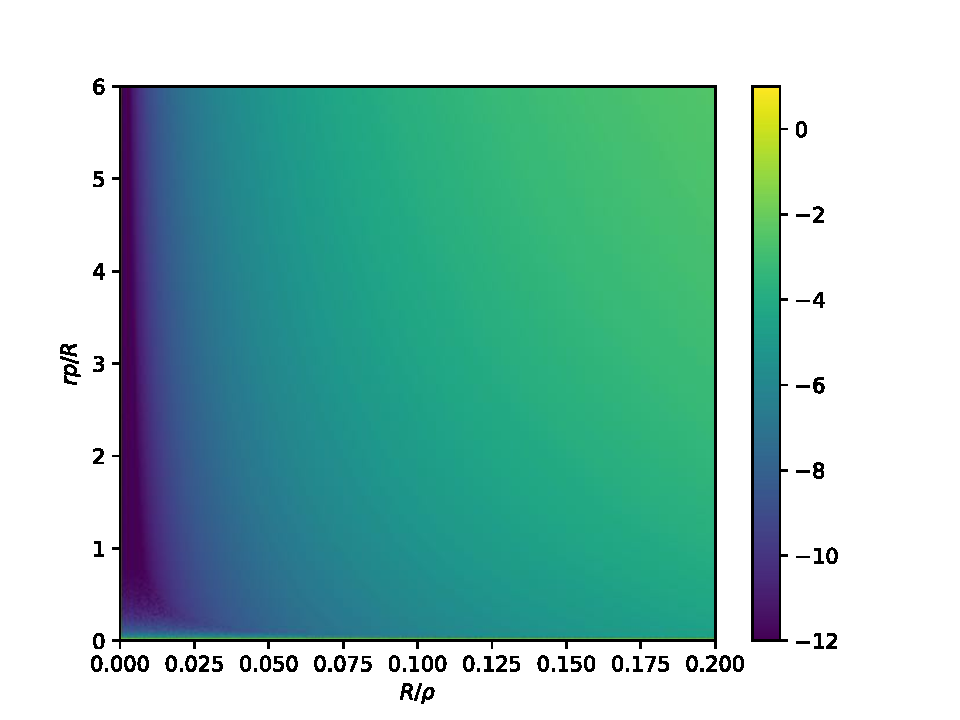
\includegraphics[width=\linewidth]{figs/extrapolation_error_plot_p6.pdf}
    \caption{\label{fig:extrap-err-p6}}
  \end{subfigure}
  \begin{subfigure}{.33\textwidth}
      \centering
      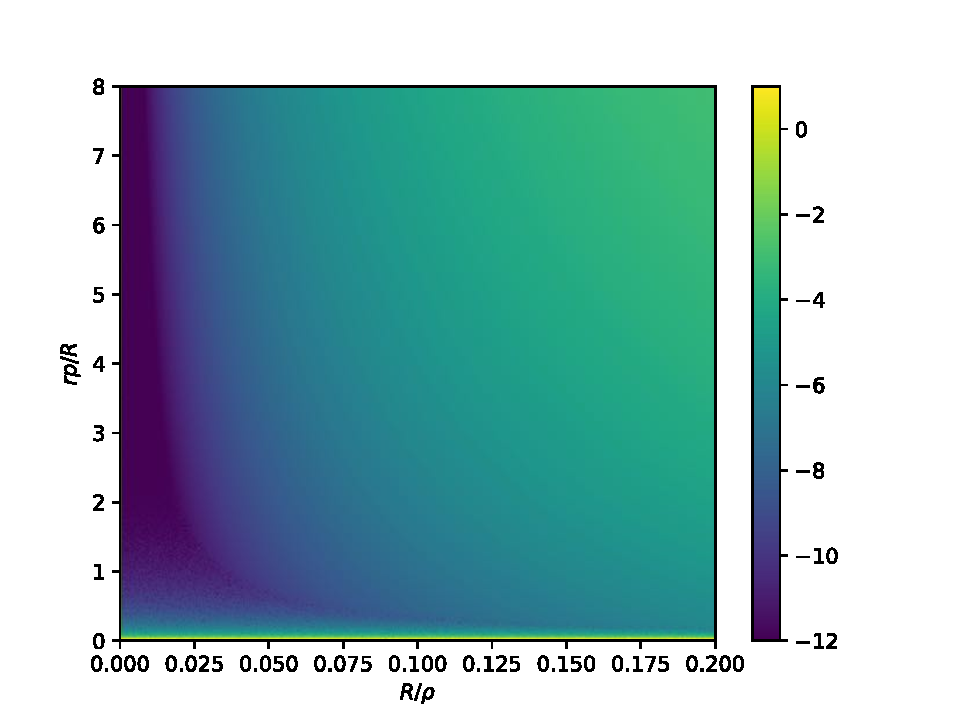
\includegraphics[width=\linewidth]{figs/extrapolation_error_plot_p8.pdf}
    \caption{\label{fig:extrap-err-p8}}
  \end{subfigure}%
    \begin{subfigure}{.33\textwidth}
      \centering
      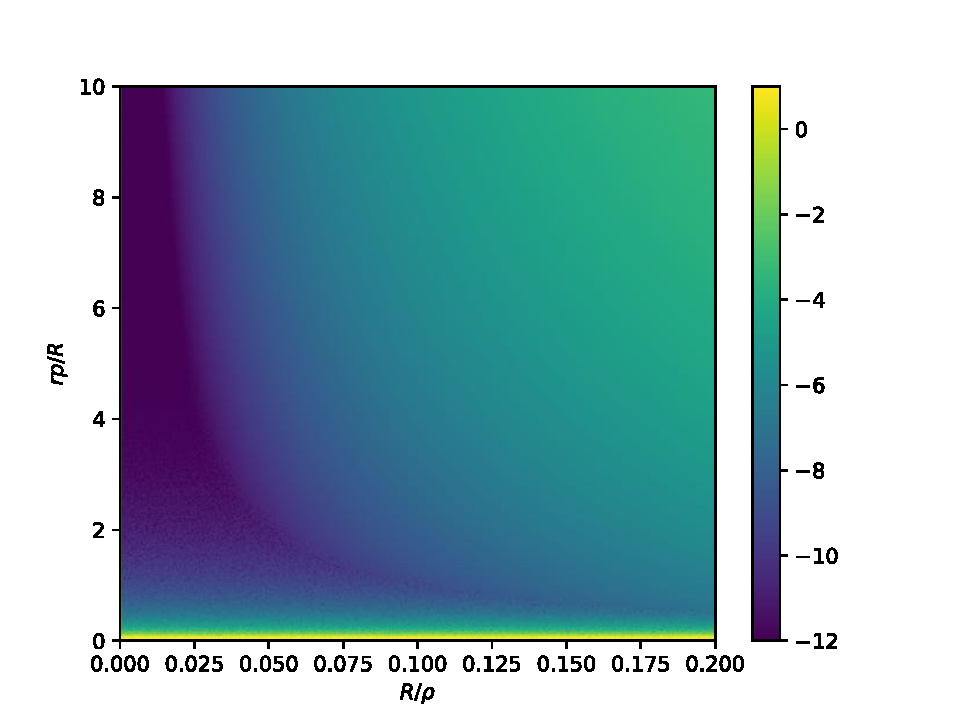
\includegraphics[width=\linewidth]{figs/extrapolation_error_plot_p10.pdf}
    \caption{\label{fig:extrap-err-p10}}
  \end{subfigure}
  \begin{subfigure}{.33\textwidth}
      \centering
      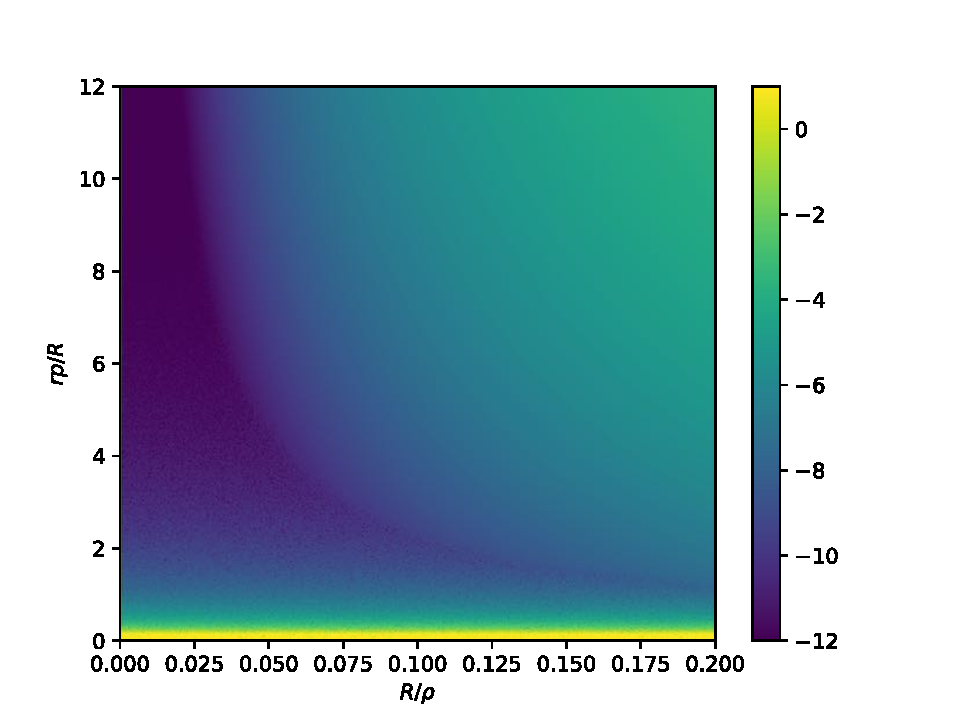
\includegraphics[width=\linewidth]{figs/extrapolation_error_plot_p12.pdf}
    \caption{\label{fig:extrap-err-p12}}
  \end{subfigure}%
  \begin{subfigure}{.33\textwidth}
      \centering
      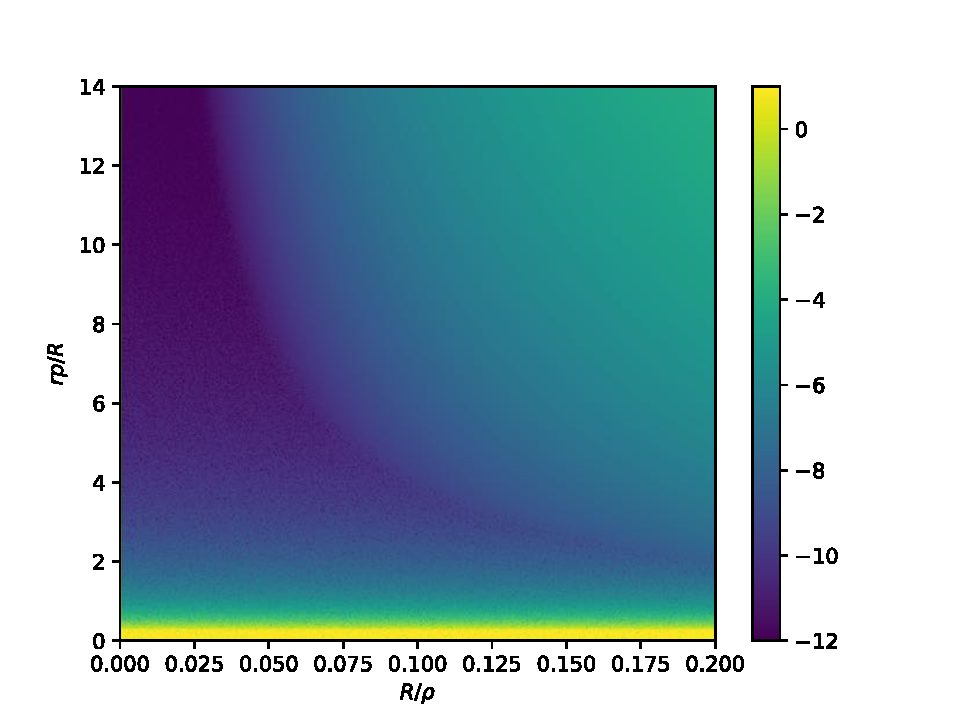
\includegraphics[width=\linewidth]{figs/extrapolation_error_plot_p14.pdf}
    \caption{\label{fig:extrap-err-p14}}
  \end{subfigure}%
  \mcaption{fig:extrap-experiment}{Empirical extrapolation error behavior}{We sweep over a range of $R$ and $r$ values to vary \Cref{fig:extrap-err-setup} and plot the log of the relative error in
    \Cref{fig:extrap-err-p6,fig:extrap-err-p8,fig:extrap-err-p10,fig:extrap-err-p12,fig:extrap-err-p14}, for values $p=6,8,10,12,14$, in increasing order, from (a) to (e).
In these figures, the $x$-axis is the extrapolation distance $R$ normalized by $\rho$ and the $y$-axis is the ratio $rp/R$.%: the total size of the approximation interval ($rp$) relative to the extrapolation distance $R$.
The top of the $y$-axis corresponds to $r=R$; $rp/R = 1$ corresponds to our choice of the parameter $a$.
Assuming that $\rho = O(L)$, $r/R = a/b$ and $R/\rho = b/\lambda$ for some constant $\lambda$.
}
\end{figure}
There are several important observations to make from these plots: 
\begin{itemize}
  \item Extrapolation error decreases as $R/\rho$ decreases, as expected.
  \item For a fixed value of $R/\rho$, the extrapolation error \textit{decreases} rapidly as $rp$ decreases, up to a certain value $r^*p$.
This is somewhat counterintuitive, since this means placing points closer together and extrapolating a further distance relative to $rp$.
For a fixed $p$ in exact arithmetic, letting the interpolation interval size tend to zero produces an order $p$ Taylor expansion of the solution $u$ centered at the interval's origin, which accounts for this phenomenon.

%\note[MJM]{Another interpretation of this result is from the perspective of Bernstein ellipses.
%Since $u$ is $C^\infty$ in a large neighborhood around the interval of interest, we can reason that the Bernstein parameter of the corresponding \oned approximation problem is growing as we decrease $rp$, thus increasing the convergence rate with respect to $R/\rho$.}

  \item Beyond $r^*p$, the extrapolation error \textit{increases}.
    The effects of finite precision eventually pollutes the convergence behavior described above. 
    Moreover, the spacing $r^*$ appears to be a function of $p$.
    For $p=6$, $r$ can be reduced to $1/p$ without any numerical issues, but
    by $p=14$, only $r>\frac{1}{2}$ is a safe choice for extrapolation.
\end{itemize}
We do not aim to rigorously analyze these phenomena in this work. 
We highlight them to provide empirical evidence that equispaced extrapolation is a reasonable, but not optimal, choice for our problem of singular/near-singular integration and to provide some intuition for our parameter choices.

The following simple result describes the behavior of the extrapolation error in \cref{eq:err-ext}.
\begin{theorem}
    Let $u(\vc(t))$ be the solution to \cref{eq:pde} given by \cref{eq:double_layer}, restricted to the line $\vc(t)$ in \threed intersecting $\vx$, let $\vc(t)$ be given by 
  \begin{equation}
    \vc(t) = \vsx - (R + tr)\vn(\vsx),
    \label{eq:check_point_param}
  \end{equation}
  where $\vsx$ is the closest point on $\Gammah$ to $\vx$, $R=bL_{\vsx}$, $r=aL_{\vsx}$, $\vn(\vsx)$ is the outward surface normal at $\vsx$, and let $|u^{(p)}(\vc(t))|$ be bounded above by $C_p$ on the interval $[-R, R+pr]$.
  Let $\mathfrak{P}(t)$ be the $p$-th order polynomial interpolant of $u(\vc(t))$ constructed from the check points $\vc_0, \hdots, \vc_p$, where $\vc_i = \vc(i)$. Then the extrapolation error associated with \qbkix behaves according to:
\begin{equation}
  |u(\vc(t_\vx)) - \mathfrak{P}(t_\vx)| \leq \frac{C_p}{(p+1)!}|R + rp|^p = \frac{C_p}{(p+1)!}|b+ap|^p\cdot | L|^p,
  \label{eq:extrap_err_init}
\end{equation}
where $t_\vx = \frac{\|\vx - \vsx\| - R}{r}$.
\label{thm:extrap_error}
\end{theorem}

\begin{proof}

    We know that for a smooth function $f$ and points $x_0, \hdots x_p$ in a \oned interval $I_0$, for some $\xi \in I_0$, the following relation holds for all $x \in I_0$:
\begin{equation}
    f(x) - \mathfrak{P}(x) = \frac{f^{(p)}(\xi)}{(p+1)!}\prod_{i=0}^p(x-x_i).
  \label{eq:exterp_err_init}
\end{equation}
Let $\mathfrak{P}$ be the $p$th order polynomial interpolating the points $x_0,\hdots x_p$.
In the \qbkix setup, since $R+rp$ is the distance of the furthest check point to $\vy$, we know that $x - x_i < R +rp$ for each $i$.
Since $f(t) = u(\vc(t))$ is harmonic, and therefore $C^\infty$, in $\Omega$, $|f^{(p)}(\xi)|$ can be uniformly bounded on $I_0$ by some constant $C_p$,
Noting that $R = bL$ and $r=aL$ yields our result.
\end{proof}

For fixed values of $a$ and $b$, as we let $L\to 0$, the extrapolation error is bounded by $O(L^p)$.
In practice, however, this means that we can choose $a$ and $b$ to minimize the constant factor $|b+ap|^p$ in \cref{thm:extrap_error}.
Since $p>1$, $a$ must be chosen to balance out the contribution of $p$, yet our extrapolation study shows that we can't simply set $a=0$.  
We therefore choose $a \leq 1/p$ for $p=6$ and 8, motivated by \cref{fig:extrap-err-p6,fig:extrap-err-p8}.
Moreover, since $b < 1$, we can choose $a \leq b/p$, which allows $a$ and $b$ to decay at the same rate.
%In exact arithmetic, $a$ controls how close the convergence order is to $p$.
%By holding $b$ fixed and letting $a\to 0$, we recover a $p$th order Taylor expansion of $u$ centered at $c_0$.
%Convergence to an approximate Taylor series is critical to the success of \qbkix and can be seen in \cref{fig:extrap-experiment}:
%we can improve extrapolation accuracy for a fixed value of $b$ by decreasing $a$, until numerical errors take over.
The advantage of choosing $a \leq b/p$ is that $b$ is a single parameter that controls the accuracy of \qbkix.
Since we have fixed the quadrature order $q=20$ to satisfy the assumption in \cref{sec:adaptive_upsampling}, a smaller value of $b$ will trigger more upsampling in \cref{alg:adaptive_upsampling}, keeping quadrature error fixed while reducing extrapolation error.

It is important to keep in mind that \cref{thm:extrap_error} only provides insight for moderate values of $p$; our conclusions are largely irrelevant for large $p$.
We use  $p = 6$ and $a = b/6$, leaving the construction of an optimal extrapolation extrapolation scheme to future work. 

\subsection{Geometry approximation error\label{sec:error_geom}}
Let $\theta$ be a scalar function defined on the surface of $\partial \Omega$ with $|\theta| \leq 1$ and let $\delta$ be a small real constant.
Suppose the boundary of the domain $\Omega$ is perturbed by $\delta$ along the normal field of $\partial\Omega$, scaled by $\theta$, to produce the perturbed domain $\Omega_\delta$ with boundary $\partial \Omega_\delta$.
More concretely, for $\vy \in \partial\Omega$ and $\vy_\delta\in \partial \Omega_\delta$, $\vy_\delta= \vy + \delta\theta\vn(\vy)$.
We can define the \textit{Eulerian shape derivative} of $u$ with respect to $\theta$, denoted $u_\theta$, at a point $\vx \in \Omega_\delta \cap \Omega$ as the rate of change in $u$ at $\vx$ as $\delta \rightarrow 0$.
This quantity is of interest to us because the solution to \cite[Equation 2]{morse2020robust} on $\Omega_\delta \cap \Omega$ can be written as $u + \delta u_\theta$, where $u$ is the solution to \cite[Equation 2]{morse2020robust} on $\Omega$.
Moreover, we can compute the shape derivative by solving a Laplace problem on the unperturbed domain \cite{pironneau1982optimal}:
\begin{equation}
\Delta u_\theta= 0\;\mbox{in $\Omega$, } u_\theta = -  \theta \frac{\partial u}{\partial n} \mbox{on $\partial\Omega$.}
\label{eq:shape-deriv}
\end{equation}  
where $u$ is the solution of the \cite[Equation 2]{morse2020robust} on $\Omega$.
For small $\delta$, this means that the error in the solution introduced by a boundary perturbation along the field $\theta$ can be estimated by  $\delta \sup_{\Omega} \| u_\theta \|$.
Assuming the boundary is smooth and the gradient of the solution $u$ is bounded, then
\begin{equation}
\| u_\theta \| \leq C_g \sup_{\partial\Omega} \left| \theta  \frac{\partial u}{\partial n} \right| \leq
C_g \sup_{\partial\Omega} \left| \frac{\partial u}{\partial n}\right|
\label{eq:shape-deriv-bound}
\end{equation}
for some real constant $C_g$.
The right-hand side of \cref{eq:shape-deriv-bound} yields a constant $C_g^\prime$, such that if $\err{g} <  \zeta\etrg/C_g^\prime$ for some $\zeta < 1$,  the change in the solution is less than $\etrg$ for a sufficiently small $\err{g}$.
%\note[DZ]{Need to find (again) a reference saying this, as this is not true for general boundaries}
The constant depends implicitly on the surface geometry: for example, if an area element of $\partial\Omega$ is close to a sharp, concave corner, then  $\frac{\partial u}{\partial n}$ can be arbitrarily large. 


\subsection{Limitations \label{sec:limitations}}
Our error discussion reveals several limitations of our method. 
The first and most apparent shortcoming is that extrapolation instability fundamentally limits convergence order. 
However, for reasonable orders of convergence, up to 14, we have discussed an empirical scheme to choose parameters to maximize the available convergence behavior.
Moreover, low-order surface geometries used in engineering applications will likely limit the convergence rate before it is limited by the extrapolation order, making this a non-issue in practical scenarios.

Another downside of the chosen extrapolation approach is lack of direct extension of \qbkix to oscillatory problems like the Helmholtz equation.
Due to the limitation on the values of $p$, we can't guarantee the ability to resolve high-frequency oscillations in the solution.
A new extrapolation procedure is required to do so robustly without compromising efficiency.

In \cite{wala20193d}, the authors demonstrate a relationship between the truncation error of a \qbx expansion and the local curvature of $\Gammah$. 
Our scheme also is susceptible to this form of error and we do not address nor analyze this in this work.
This is a subtle problem that requires a detailed analysis of the surface geometry with respect to the chosen extrapolation scheme.
%We leave this to a future work that produces an optimal extrapolation approach in the boundary integral context.
Another  limitation is the lack of an accurate error estimate to serve as an upsampling criteria in place of the criteria in \cref{sec:adaptive_upsampling}, such as \cite{klinteberg2019accurate}. 
Extending \cite{klinteberg2019accurate} to \threed surfaces is non-trivial and whether the size of $\Pfine$ would be reduced enough to outweigh the added cost of the additional Newton iterations required by their scheme remains to be seen.

Finally, for certain accuracy targets and geometries, the algorithm above may lead to an impractically high number of patches in $\Pcoarse$ and $\Pfine$. 
Geometries with nearly-touching non-local regions, as shown in \cref{fig:torii}, will see large amounts of refinement.
If the nearly-touching embeddings $\gamma_r$ are close enough, i.e., less than $10^{-10}$ apart, there is little hope of an accurate solution with a fixed computational budget.
We allow the user to enforce a minimal patch size $L_\lbl{min}$, limiting the time and memory consumption at the expense of not reaching the requested target accuracy. 


\section{Complexity Analysis\label{sec:complexity}}
In this section, we analyze the complexity of the algorithms required by \qbkix. 
The input to our overall algorithm is a domain boundary $\Gamma$ with $\Ninit$ patches and boundary condition $f$.
We begin with a summary of algorithm parameters that impact complexity: 

\begin{itemize}
\item The number of patches $N$ \emph{after} admissibility refinement.  
  This is a function of $\Ninit$, the geometry of $\Gamma$, the definition of $f$, and the choices of parameters $a$ and $b$ in check point construction. 
\item Quadrature order $q$ and the degree of smoothness $k$ of $\Gamma$ and $f$.
  We assume that $k$ is sufficiently high to obtain optimal error behavior for a given $q$ by letting $k=2q$ in \cref{eq:error_quad_gen_target}.
\item \qbkix interpolation order $p$. 
\item The numbers of evaluation points in different zones $\Nf$, $\Ni$, and $\Nn$, with $\Nt = \Nf+\Ni+\Nn$.
%\item Maximum upsampling ratio $m = \max_i m_i$, where $m_i$ is the upsampling ratio for the $i$-th patch.
%\item Target error $\etrg$ used to determine check point location.
\end{itemize}

%The complexity is also affected by the geometric characteristics of the surface. These include maximum patch size $\Lmx$, relative minimal patch size $\Lmn = \beta_0 \Lmx$, $\beta_0 \leq 1$, as well as \emph{minimal feature size} $\ellm = \alpha_0\Lmx$ and \emph{the variation of area distortion} of the parametrization $C_J$, which we now define more precisely.  
%The local feature size $\ellm$ is defined in terms of the \emph{medial axis} of the surface.  The medial axis of a surface $\Gamma$, $M(\Gamma)$, is the set of points in $\mathbb{R}^3$ with more than one closest point on $\Gamma$. For $\vx \in\Gamma$, the local feature size  $\ell(\vx)$ is the distance from $\vx$ to $M(\Gamma)$. We assume that the minimal feature size \emph{relative to $\Lmx$} is bounded from below by $\alpha_0$, i.e., $\ell(\vx) \geq \alpha_0 \Lmx$.  
%The variation of the area distortion $C_J(P)$ is $\max_{(u,v)} |J|/\min_{(u,v)} |J|$, where $J$ is the Jacobian of the patch parametrization for an initial patch $P$, and $C_J$ is the maximum of $C_J(P)$ over all patches; this constant indicates how nonuniform the parametrization is, and allows us to estimate how the patch size decreases with refinement \note[MJM]{add a sentence with example: high $C_J$ vs. low $C_J$}. 
%We assume that the $\alpha_0$, $\beta_0$ and $C_J$ are independent of $N^{init}$. We also assume that surface principal curvatures are bounded, independently of $N^{init}$. 
The complexity is also affected by the geometric characteristics of $\Gamma$. 
These include:
\begin{itemize}
  \item The \textit{maximum patch length} $\Lmx = \max_P L(P)$
  \item The \textit{relative minimal patch length} $\Lmn = \beta_0 \Lmx$, $\beta_0 \leq 1$.
  \item The \textit{minimal feature size relative to $\Lmx$}, $\ellm = \alpha_0\Lmx$, which is defined in terms of the \textit{local feature size} and the \textit{medial axis} of $\Gamma$.
The medial axis of $\Gamma$, denoted $M(\Gamma)$, is the set of points in $\mathbb{R}^3$ with more than one closest point on $\Gamma$. 
For $\vy \in\Gamma$, the local feature size  $\ell(\vy)$ is the distance from $\vy$ to $M(\Gamma)$.
We assume that the local feature size is bounded below by $\alpha_0\Lmx$, i.e., $\ell(\vy) \geq \alpha_0 \Lmx = \ellm$ for $\vy \in \Gamma$.
  \item The \emph{maximum variation of area distortion} of the parametrization $C_J$.
The variation of the area distortion of a patch $P$ is $C_J(P) = \max_{(u,v)} |J_P(u,v)|/\min_{(u,v)} |J_P(u,v)|$, where $J_P(u,v)$ is the Jacobian of $P$ at the point $(u,v)$. 
We define $C_J = \max_{P\in\Gamma} C_J(P)$.
This value is an indicator of how non-uniform the parametrization of $P$ is and allows us to estimate how the patch length decreases with refinement. 
\end{itemize}


We assume that the $\alpha_0$, $\beta_0$ and $C_J$ are independent of $\Ninit$. 
We also assume that principal curvatures are bounded globally on $\Gamma$ and independent of $\Ninit$. 
We now briefly summarize the results of this section:

\begin{itemize}
\item \emph{Admissibility.} (\cref{sec:complexity_admissibility}) The complexity of this step is $O(\Ninit \log \Ninit)$,
  with constants dependent on $\alpha_0$, $\beta_0$ and $C_J$. 
  The logarithmic factor is due to use of an \aabb tree for closest surface point queries. 

\item \emph{Upsampling.} (\cref{sec:complexity_upsampling}) The complexity of upsampling is $ O(m  N \log(N))$, where $m$ is the upsampling ratio.
  The logarithmic factor appears for similar reason to admissibility,
  with constants that depend on geometric parameters and the boundary condition through the error estimate of \cref{sec:error}.
  We show that the upsampling ratio is independent of $N$.
  %The upsampling ratio is $m = O(\etrg^{-1/q})$.
  
\item \emph{Point marking.} (\cref{sec:complexity-point-marking}) Identifying which zone an evaluation point belongs to ($\Omega_F, \Omega_I$ or $\Omega_N$) depends on $N$ and the total number of points to be classified $\Nt = \Nf + \Ni + \Nn$. 
  The complexity is $O(\Nt \log N)$ with constants dependent on geometric parameters, due to the cost of closest surface point queries. 
  
\item\emph{ Far, intermediate and near zone integral evaluation.} (\cref{sec:complexity_matvec}) The complexity of these components depends on $N$ and  $\Nf$, $\Ni$ and $\Nn$ respectively, with the general form $O(s_1 N + s_2 N')$, where $N'$ is the number of evaluation points in the corresponding class.  For the far field, $s_1 = s_2 = 1$.  For the intermediate evaluation,
$s_2 =1$, and $s_1 = m q^2$; finally, for the near zone, $s_2 = p$, and $s_1 = mq^2$, the same as in the intermediate zone.  
If $b$ is chosen appropriately, the intermediate and near zone error is $\etrg$. 

  %\note[DZ]{This is not quite true: we should probably modify the upsampling alg description, so that we actually get
  %  this in the near zone, not just intermediate; otherwise it is a pain to explain, as there is also the extra dependence on the extrapolation order, so smth like $(\Lmx*2^\eta_1)^q$}
  %  \note[MJM]{fix} 
  \item \emph{\gmres solve.} Due to the favorable conditioning of the double-layer formulation in \cref{eq:int-eq}, \gmres converges rapidly to a solution in a constant number of iterations for a given $\Gamma$ that is independent of $N$. 
    This means that the complexity to solve \cref{eq:int-eq} is asymptotically equal (up to a constant dependent on $\Gamma$) to the complexity equal to a near-zone evaluation with $\Nn=N(q+1)^2$. 
\end{itemize}


\subsection{Admissibility \label{sec:complexity_admissibility}}

The patch refinement procedure \cref{sec:admissible} to enforce \cref{criteria:1,criteria:2} of admissibility and achieve given approximation errors of the geometry $\err{g}$ and boundary data $\err{f}$ is a local operation on each patch.
If we assume that $\Lmn$, $\Lmx$, the partial derivatives of all patches composing $\Gammah$, and the partial derivatives of $f$ are bounded, then 
 errors $\err{g}$ and $\err{f}$ can always be achieved after a fixed number of refinement steps. As a consequence, this stage must have complexity $O(\Ninit)$. 


We focus on the additional refinement needed to satisfy \cref{criteria:3}: ensuring that each check center $\vhc$ is closest to its corresponding quadrature point $\vy$. 
This can be restated in terms of local feature size: for a quadrature patch $P \in \Gamma$ and quadrature node $\vx \in P$ with check center $\vhc$, $\|\vx - \vhc\|_2 \leq \ell(\vx) \leq \alpha_0 L_0$. 
We will first relate the number of required refinement steps $\eta$ to satisfy \cref{criteria:3} to the shape parameters $\alpha_0$ and $C_J$, then we will show that this number does not depend on $N$ under our assumptions.

Recall that the distance from a check center to the surface  for a patch $P$ is given by
$R + r(p+1)/2 = (a+ (p+1)b/2)L(P)= K L(P)$. %, where $L(P)$ is the square root of the area of $P$.
After $\eta$ refinement steps, the area of each child of $P$ relative to $P$ itself will have decreased by at least by $C_J(P)(1/4)^\eta$.  
Since the distance from $\vhc$ to the surface is proportional to $L(P)$, we can estimate the required level
of uniform refinement to satisfy \cref{criteria:3} by requiring that the check center distance is less than the minimal local feature size, then taking the maximum value of $L(P)$ over all patches:
\[
K \Lmx \sqrt{C_J} (1/2)^\eta \leq \ellm = \alpha_0 \Lmx
\]
This yields

\begin{equation}
  \eta   =  \lceil -\log_2 \frac{\alpha_0}{K \sqrt{C_J}}\rceil,
\label{eq:eta-estimate}
\end{equation}
which we note depends only on nondimensional quantities $\alpha_0$, $K$ and $C_J$ characterizing the shape of the surface and its parametrization.  
If we assume these to be independent of $N$, then
the number of required levels of refinement $\eta$ are also independent of $N$. 
This means that the number of patches $N$ generated \cref{alg:admissibility} is a linear function of $\Ninit$, bounded by $4^{\eta} \Ninit$.

Next, we estimate the complexity of work per patch in \cref{alg:admissibility} to determine if a given patch requires refinement. 
As described in \cref{sec:admissible}, for each patch, we query the \aabb tree $T_B$ for patches that are at the distance $R + r(p+1)/2 = K L(P)$ from a check center $\vhc$.
The cost of the query is logarithmic in the number of patches $\Ninit$ and proportional to the number of patches $N(\vhc)$ returned.  
This means that we need to estimate the number of patches that can be within the distance $K L(P)$ from $\vhc$.

Consider an area element $dA$ of $\Gammah$ at a point $\vx_0$. The parallel surface of $dA$,
given by $\vx_0 + h \vn(\vx_0)$ does not have self-intersections when $|h| \leq \ellm$ and has a corresponding area element given by $dA^{h} = (1+ h \kappa_1)(1+h \kappa_2)dA$ \cite[Section 6.2]{K}, where $\kappa_1$ and $\kappa_2$ are the principal curvatures of $\Gammah$ at $\vx_0$.
The volume of the truncated cone bounded by $dA$ and $dA^{h}$ of height $\ellm$ can be computed directly from the integral $\int_0^{\ellm} dA^h dh$:
\[
  dV = dA \ellm (1 + \frac{1}{2} (\kappa_1 + \kappa_2) \ellm + \frac{1}{3} \kappa_1 \kappa_2 \ellm^2)   = dA\ellm(1 + \frac{1}{2} H \ellm + \frac{1}{3} K \ellm^2)
\]
where $K$ and $H$ are Gaussian and mean curvatures respectively. As principal curvatures satisfy
$\kappa_i \geq -1/\ellm$,  this expression has minimal value for $\kappa_1 = \kappa_2 = -1/\ellm$:
\begin{equation}
dV \geq \frac{1}{3}\ellm dA
\label{eq:vol-lower-bound}
\end{equation}
In other words, each surface element $dA$ has (at least) a volume $\frac{1}{3}\ellm dA$ with no other surface elements inside associated with it.  From this, we can estimate the total area of surface contained within distance $K L(P)$ from $\vhc$ by equating \cref{eq:vol-lower-bound} with the volume of a sphere of raidus $KL(P)$, producing $4 \pi K^3 L(P)^3/\ellm$.
Since the area of each patch is at least $L_{\min}^2$, the number of patches $KL(P)$ from $\vhc$ is bounded by

\begin{equation}
  N(\vhc) \leq  4 \pi K^3 \frac{L(P)^3}{\ellm \Lmn^2} \leq 4 \pi K^3 \frac{\Lmx^3}{\ellm \Lmn^2} =
  \frac{4 \pi K^3}{\alpha_0 \beta_0^2}
 \label{eq:numpatches-estimate}
 \end{equation}

This is independent of $\Ninit$, which means that the complexity of nearest patch retrieval is $O( \Ninit \log \Ninit)$, with constant given by the product of
\eqref{eq:numpatches-estimate} and $4^\eta$, with $\eta$ given by \eqref{eq:eta-estimate}.

To complete the complexity estimate of the admissibility refinement, we need to estimate the cost of computing the closest point on each patch.
The complexity of the Newton's method for finding roots of polynomials  in \cref{app:closest_point} depends only on the polynomial degree and the desired accuracy of the optimization, which we can assume to be bounded by floating-point precision \cite{schleicher2017newton}.
We conclude that the overall complexity of admissibility refinement is $O( \Ninit \log \Ninit)$ with constants proportional to the patch degree and optimization accuracy.

\subsection{Upsampling\label{sec:complexity_upsampling}}
We estimate the complexity of the upsampling algorithm in \cref{sec:adaptive_upsampling} in terms of $N$, the number of patches produced by admissibility refinement, and a parameter $\eps$, which is the desired accuracy achieved by the final upsampled patches at the check points.
As the distance from the surface to the check points $\vc_i$ is bounded from below by
$a \Lmn$,  the $\tilde{V}$ term 
in \cref{eq:error_quad_gen_target} is bounded from above by $C \Lmn^{-2q-1}$, for a constant $C$ independent of $q$. 
Furthermore, since $\Gammah$ and $f$ are assumed to be smooth, the density and its derivatives can also be assumed to be bounded.
The overall form of the estimate in \cref{eq:error_quad_gen_target} can then be bounded and written as $\tilde{C}(q) \Lmn^{-2q-1} \tilde{L}^{2q}$ for some constant $\tilde{C}(q)$. 
The maximum patch length obtained by refinement $\tilde{L}$ is 
\begin{equation}
  \tilde{L} = \Lmx^\lbl{fine} \leq \Lmx 2^{-\tilde{\eta}},
  \label{eq:Ltilde}
\end{equation}
where $\tilde{\eta}$ is the maximum amount of required patch refinement.
By setting $C(q) \Lmn^{-2q-1} \tilde{L}^{2q} \leq \eps$ and using \cref{eq:Ltilde}, we can 
obtain an upper bound for $\tilde{\eta}$ as a function of $\Lmn$, $\Lmx$, and $\eps$:
\begin{equation}
  \tilde{\eta} \leq -\frac{1}{2q}\log_2 \left( \frac{\eps}{\Lmn^{-2q-1} \Lmx^{2q} C(q)}\right)= \log_2 \eps^{-1/(2q)} + \bar{C}(q,\Lmn,\Lmx),
  \label{eq:tildeeta}
\end{equation}
for some constant $\bar{C}(q,\Lmn,\Lmx)$.

The number of points generated by upsampling is $O(4^{\tilde{\eta}} N )$.
Taking powers of both sides of \cref{eq:tildeeta} yields an
estimate in terms of $\err{target}$:  $O( (2^{\tilde{\eta}})^2N ) \leq O(\eps^{-2/(2q)}N ) =  O(\eps^{-1/q}N )$. 
As discussed in \cref{sec:complexity_admissibility}, the closest point computation needed to determine if a checkpoint is in $\Omega_I$ has $\log (N)$ cost per point, leading to $O(\eps^{-1/q} N \log(N))$ overall complexity and an upsampling factor of $\eps^{-1/q}$. 
Since we desire upsampled quadrature with an accuracy of $10^{-12}$, we set $\eps$ as such to arrive at the desired complexity.


%Note that both $C$ and $\tilde{C}(q)$ above depend on higher-order derivatives of the patch $P$ and therefore implicitly on principal curvatures $\kappa_1$ and $\kappa_2$.
%This partial explains the difference in accuracy between \cref{eq:error_quad_gen_target} and \cref{eq:rem2d_heuristic}.
%In practice, we use the more precise error bound \cref{eq:rem2d_heuristic}, so the actual refinement is less than \cref{eq:error_quad_gen_target} might suggest in this analysis

\subsection{Point marking\label{sec:complexity-point-marking}}
In the point marking algorithm of \cref{app:point_marking}, we first use the Laplace \fmm to cull points far from $\Gamma$, which requires $O(N+\Nt)$ time. 
Let $\bar{L} = \frac{1}{M}\sum_{P \in \Pcoarse}L(P)$ be the average patch length.
After \fmm culling, the remaining unmarked evaluation points are those whose distances from $\Gamma$ are approximately $\bar{L}$ or less.  For each unmarked point $\vx$,  we query the \aabb tree $T_T$ for the nearest triangle in the linear approximation of $\Pcoarse$.

Since there are $O(N)$ such triangles in $T_T$, we can perform this query in $O(\log N)$ time \cite{samet2006foundations}.
This triangle provides a candidate closest patch that is distance $d_0$ from $\vx$. 
We then use to query $T_B$ for all bounding boxes at distance $d_0$ from $\vx$.  
This query too can be performed in $O(\log N)$ time \cite{samet2006foundations} and returns a bounded number of boxes and that each is processed in constant time, as discussed in \cref{sec:complexity_admissibility}.
As the number of unmarked points after culling is bounded above by $\Nt$, the overall complexity of our marking scheme is $O(\Nt \log N)$.


\subsection{Integral evaluation complexity \label{sec:complexity_matvec}}
We assume that geometric admissibility criteria are already satisfied. 
All integral evaluation is accelerated using an \fmm with complexity $O(N + \Nt)$. 
\paragraph{Far zone}  The complexity of far evaluation is just the complexity of computing the integrals on $\Pcoarse$ using standard quadrature and \fmm acceleration, i.e.,  $O(q^2N + \Nf)$.% \sim O(n^2N + \Nf)$.

\paragraph{Intermediate zone} The complexity of the intermediate zone evaluation is similar to that of the far zone.
However the computation is performed on $\Pfine$ rather than $\Pcoarse$, which is up to $m$ times finer than $\Pcoarse$,  with $m = O(\eps^{-1/q})$ and $\eps=10^{-12}$.
The density values must be interpolated from points in $\Pcoarse$ to points in $\Pfine$: this can be computed in $O(mq^4N)$ time using a \twod version of the barycentric interpolation formula \cite{BT}.
This yields an overall complexity of  $O(mq^4N + m q^2N + \Ni)$.
Although not asymptotically dominant, for all practical target errors, the quadrature evaluation is the dominant cost in practice due to suppressed \fmm-related constants, as demonstrated in \cref{sec:results-compare}.

\paragraph{Near zone} %In our algorithm, the near zone includes points on the surface itself. 
\cref{sec:singular-eval} requires a closest point computation, an intermediate-zone evaluation at $p$ check points and an extrapolation for each target point in $\Omega_N$.
The intermediate zone calculation is the dominant cost, resulting in a complexity of $O(mq^4N + m q^2 N + p\Nn)$.

\paragraph{\gmres solve} As a result of the second-kind integral formulation in \cref{sec:formulation}, the cost of solving \cref{eq:int-eq} via \gmres is asymptotically equal to the cost of a single singular integral evaluation, since the low number of iterations are independent of $N$.  
In our algorithm, this is a special case of near-zone evaluation with $\Nn = q^2N$, producing a complexity of $O(mq^4N + mq^2N + pq^2N) =O( (m+p+mq^2) q^2 N)$. 

\paragraph{Overall complexity for uniform point distribution}
We now suppose that we wish to evaluate the solution $u$ determined by a density $\phi$ at a set of uniformly distributed points throughout $\Omega$.
We also assume that $\Gammah$ is discretized uniformly by $N$ patches, i.e., $\Lmx = O(N^{-1/2})$ and that the distances between samples in $\Omega$ and from samples to $\Gammah$ are also $O(N^{-1/2})$.
Since the total number of evaluation points is proportional to $1/\Lmx^3$, this implies that $\Nt = O(N^{3/2})$.

The size of the intermediate zone $\Omega_I$ is bounded by the estimate discussed in \cref{sec:complexity_upsampling}.
Letting $d_I$ be the shortest distance along a normal vector of $\Gammah$ which is contained in $\Omega_I$, following the discussion in \cref{sec:complexity_upsampling} yields the following relation:
\begin{equation}
  \tilde{C}(n) d_I^{-2q-1} \Lmx^{2q} \leq \eps.
\end{equation}
Solving for $d_I$ gives us
\begin{equation}
  d_I \leq \left(\frac{\eps}{C(n)}\right)^{-\frac{1}{2q-1}} \left(\Lmx\right)^{\frac{2q}{2q-1}}.
\end{equation}
We are interested in the regime as $N \to \infty$, or $\Lmx \to 0$.
Since $\Lmx^{\frac{2q}{2q-1}} \leq \sqrt{\Lmx} = O(N^{-1/4})$, this gives us 
\begin{equation}
  d_I \leq \left(\frac{\eps}{C(n)}\right)^{-\frac{1}{2q-1}} N^{-1/4} = O(\eps^{-1/2q}N^{-1/4}) = O(\sqrt{m}N^{-1/4}),
\end{equation}
after recalling from above that $m = O(\eps^{-1/q})$ is the average upsampling rate to produce $\Pfine$ from $\Pcoarse$.
The size of the near zone is, by construction, of the order $\Lmx$.
It follows that $\Ni =O(  \sqrt{m} N^{5/4})$, and $\Nn =O(N)$.

The overall complexity for this evaluation is the sum of the cost of each separate evaluation: 
\begin{align*}
  &O(q^2N + \Nf + mq^4 N + mq^2 N + \Ni + mq^4 N + mq^2N + p\Nn)\\
  %&= O((m + mq^2)q^2N + \Nf + \Ni  + p\Nn)\\
  &= O\left( (m+mq^2)q^2N + \Nt + (p-1)\Nn \right)
\end{align*}
Using the estimates for $\Nt$ and $\Nn$ and dropping dominated terms, we obtain  $O( (m + m q^2)q^2 N + N^{3/2})$ for the overall complexity.
This suggests that for a given $q$ and $\eps$, the minimal cost is obtained from choosing the number of discretization points 
$N =O(m^2)$, i.e., $ N = O(\eps^{-2/q})$. 

%The overall complexity, $O(n^2N + \Nf + mn^2 N + \Ni + n\Nn  + (m+n) n^2 N)$,
%i.e., $O( (m + n)n^2 N  + \Ni + n \Nn + \Nf) = O( (m+n)n^2 N + \Nt + (n-1)\Nn)$.  
%Using the estimates for $\Nt$ and $\Nn$,
%we obtain, dropping  dominated terms,  $O( m n^2 N + N^{3/2})$ for the overall complexity.
%This suggests that for a given target error $\etrg$, the minimal cost is obtained from choosing the number of surface points
%$N \sim m^2$, i.e., $\etrg^{-4/n}$. 




\iffalse
\subsection{AABB Tree complexity}
It is a non-trivial task to prove that an AABB tree query has logarithmic complexity with respect to the number of contained boxes for general geometries in 3D.
Since the location of bounding boxes are a function of $\Gamma$, they have no well-defined spatial partition in general; this makes it challenging to make claims about the tree depth.
This is a research topic in its own right \note[MJM]{list two recent-ish papers}.
However, Proposition 1 of \cite{RKO} similarly applies to AABB trees:
\begin{proposition}
  Any query of an AABB tree requires in $O(d+n_\lbl{box})$ work, where $d$ is the number of levels in the tree, and $n_\lbl{box}$ is the number of bounding boxes returned from the query.
  \label{}
\end{proposition}
\note[MJM]{we can comment about how no closed boundary can have the worst case complexity of \cite{hammer2002box} globally, but i don't think we can prove $log(N)$ time}.

\subsection{Complexity comparison with \cite{YBZ}}
\note[MJM]{some comments about why we're only looking at one solver, not sure how to justify}
We compare \qbkix with the singular quadrature scheme of \cite{YBZ}, which we will refer to as \textit{partition of unity quadrature}, or \pou quadrature.
This scheme is quite different from the \qbkix method presented in this work; we summarize the key differences to avoid confusion.
\note[MJM]{add image highlighting difference in discretization, overlapping vs non overlapping}
In \cite{YBZ}, $\Gamma$ is defined as a set of compactly supported overlapping patches, detailed in \cite{ying2004simple}.
Each patch is discretized with a periodic tensor-product trapezoidal rule with spacing $h$.
The potential is computed at all discretization points, then a new partition of unity function $\eta(\vx)$, centered at the target point, is used to subtract the inaccurate near contribution.
$\eta(\vx)$ is then integrated with a periodic polar trapezoidal rule, which cancels the singularity by centering the polar grid at the target, and added to the accumulated potential.

The complexity of this algorithm is $O(N^{3/2})$, because the number of points used in the polar trapezoidal rule for each target point is $O(\sqrt{N})$. 
Asymptotically, \qbkix will outperform \pou quadrature.
However, consider that the dominant cost of \qbkix is the \fmm evaluation of size $O(kN + pN)$; meanwhile, the \fmm evaluation of \pou quadrature is simply $O(N+N)$, since the source and targets are equal.
This also implies that the size of the \fmm tree for \pou quadrature is smaller than for \qbkix, whose source and target points are more distributed in space.
For small values of $N$ and low target accuracies, we can expect \pou quadrature to have a shorter \fmm setup and evaluation time than \qbkix, and therefore a lower overall runtime.

\fi

% body
\section{Results\label{sec:results}}
We now demonstrate the accuracy and performance of \qbkix to evaluate singular/near-singular layer potentials on various complex geometries to solve the integral equation in \cref{eq:int-eq} and evaluate the solution as defined in \cref{eq:double_layer}.

\subsection{Classical convergence with patch refinement}
We will first demonstrate the numerical convergence behavior of \qbkix.
As discussed in \cite[Section 3.1]{KBGN}, approximation-based schemes such as \qbkix do not converge classically but do so up to a controlled precision if $r$ and $R$ scale with proportional to the patch size. 
In order to observe classical convergence as we refine $\Pcoarse$, we must allow $R$ and $r$ to decrease slower than $O(L)$, such as with rate $O(\sqrt{L})$.
In this section, we choose the \qbkix parameters $a$ and $b$ proportional to $1/\sqrt{L}$ to achieve this and demonstrate numerical convergence with refinement of $L$.

In our examples, we use analytic solutions to \cref{eq:pde} obtained as sums of point charge functions of the form 
\begin{equation}
  u_c(\vx) = \sum_{i=1}^m G(\vx,\vy_i)\psi_i
  \label{eq:point-charge-solution}
\end{equation}
%are solutions to \cref{eq:pde} by construction, 
where the charge locations $\vy_i$ with strengths $\psi_i$ are outside of $\Omega$.
To construct specific solutions, we sample a sphere of radius one with point charges, as shown in \Cref{fig:greens-id-test-cases,fig:solver-conv-test-cases}.
We choose charge strengths $\psi_i$ randomly from $[0,1]^d$, where $d=1$ for Laplace problems and $d=3$ for Stokes and elasticity problems. 

We use the multipole order  $m=20$ with $5000$ points per leaf box for the  kernel-independent \fmm. 
This ensures that the \fmm error does not dominate;  sufficiently large number of points per leaf box is needed to minimize the additional error due to tree depth.
We choose a high quadrature order $q=20$, or 400 quadrature points per patch in $\Pcoarse$, relative to overall convergence order to satisfy the assumption in \cref{sec:adaptive_upsampling}.
We also use two levels of uniform upsampling to demonstrate convergence.


\subsubsection{Green's Identity}
\begin{figure}[!htb]
  \centering
  \begin{minipage}{.5\textwidth}
      \centering
    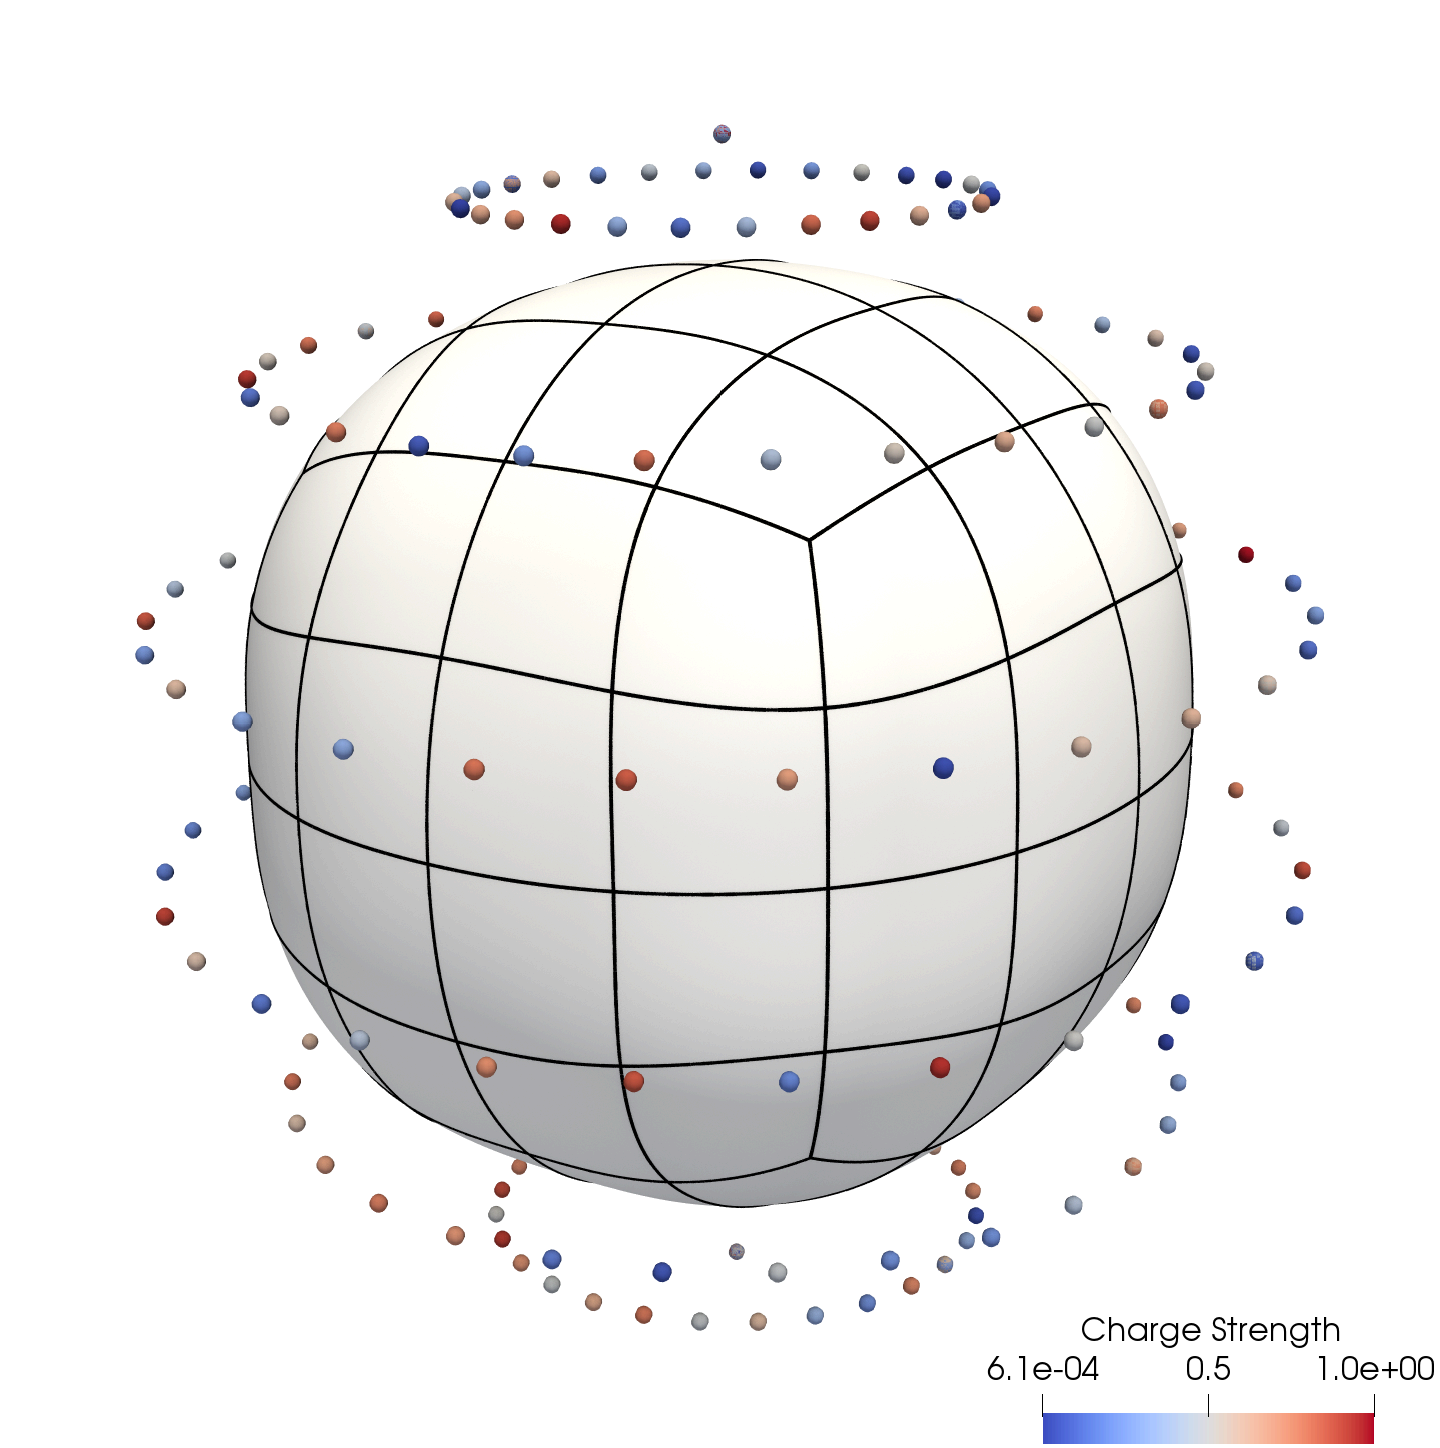
\includegraphics[width=.75\linewidth]{figs/cube_convergence_setup}
  \end{minipage}\hfill
  \begin{minipage}{.5\textwidth}
      \centering
    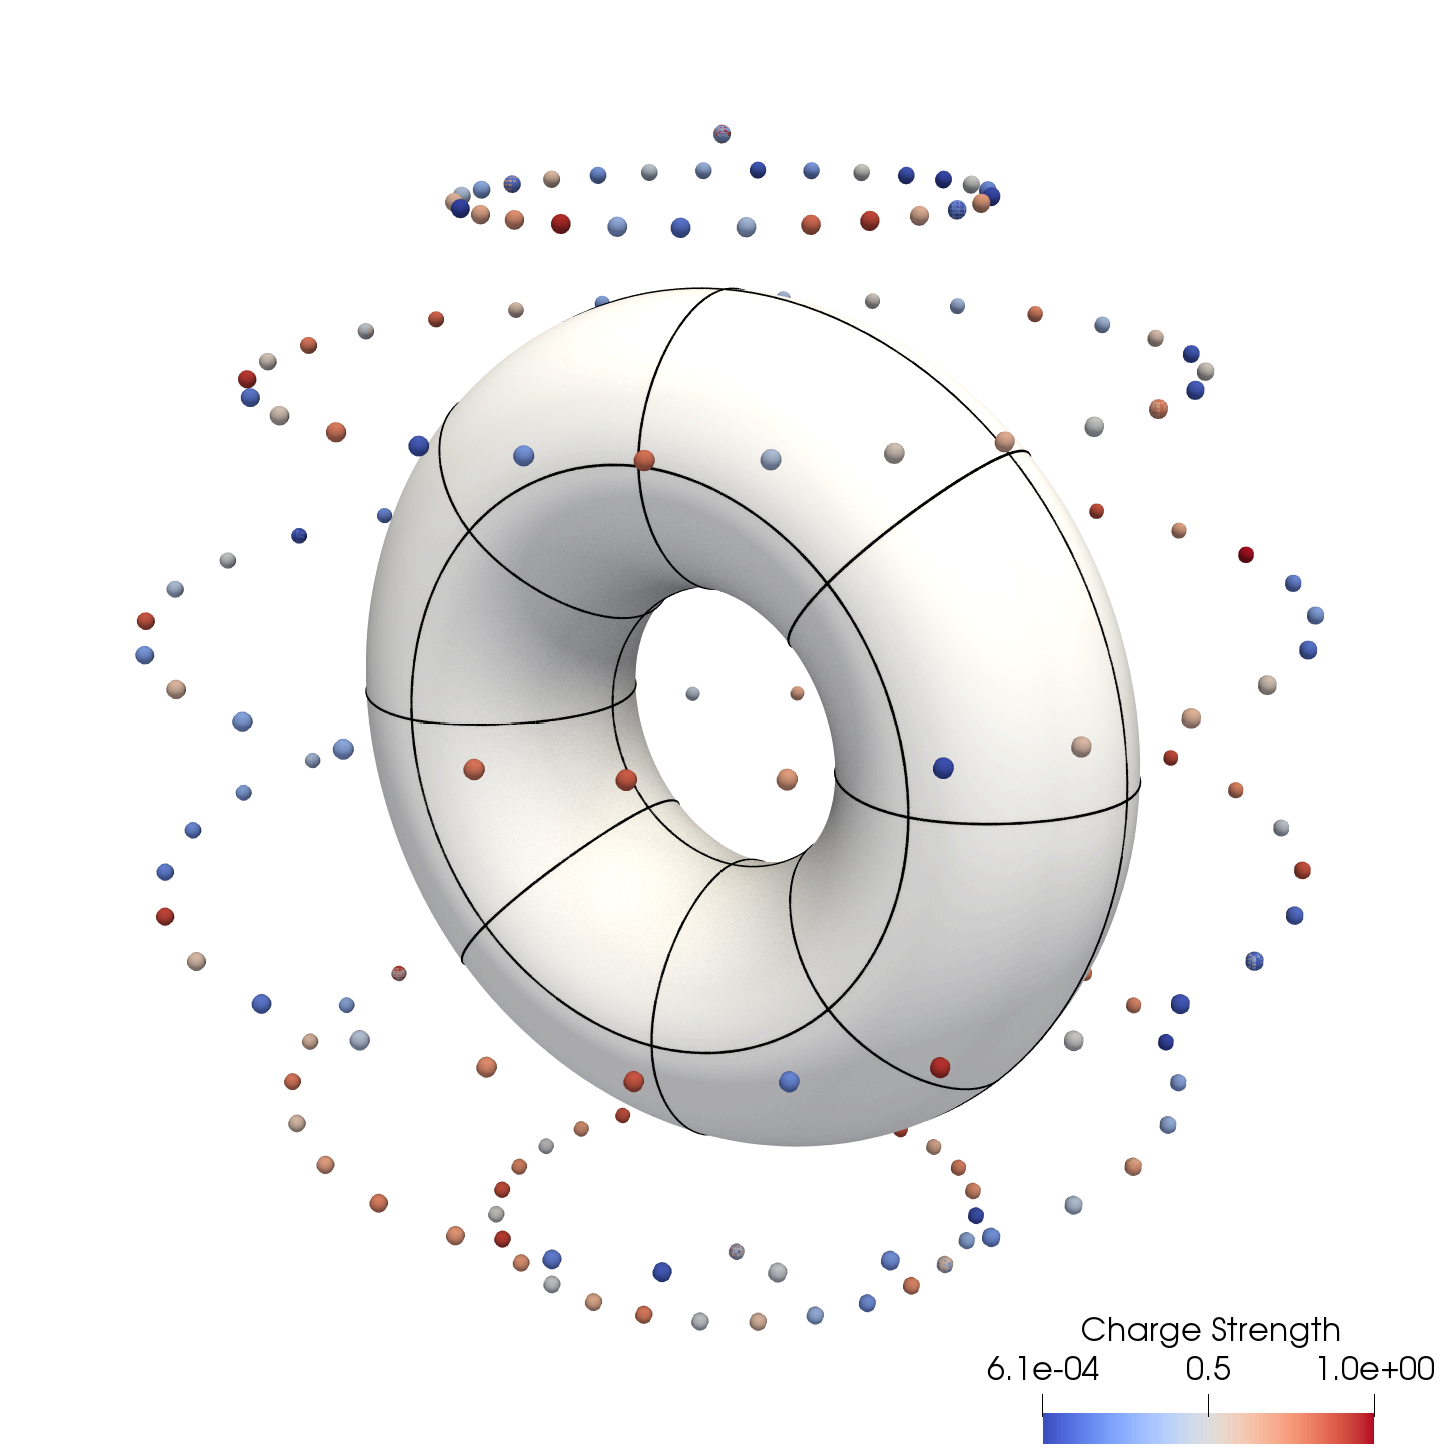
\includegraphics[width=.75\linewidth]{figs/newtorus_convergence_setup}
  \end{minipage}\hfill
  \mcaption{fig:greens-id-test-cases}{}{Geometry and singularities used for Green's Identity convergence tests. 
  Shown are polynomial patches defining boundary geometry (black lines) and point singularities
  placed on the surface on a sphere of radius one.
  Singularity strengths are randomly selected values in $[0,1]$; shown is the strength intensity for Laplace problems, which varies from blue to red.
  We use 96 20th-order polynomial patches for the spheroid (left) and 32 cubic patches for the torus (right).
}
\end{figure}

\begin{table}[!htb]
\centering
\small
\setlength\tabcolsep{4pt}
\begin{tabular}{lllllll}
\toprule
{}Geometry & \pde &\multicolumn{4}{c}{Relative $\ell^\infty$ error (Number of patches)} & EOC\\
\midrule
Spheroid                                    & Laplace         &  $1.06\times 10^{-4}$ (96) &  $4.78\times 10^{-6}$ (384) &  $9.14\times 10^{-8}$ (1536) &  $4.35\times 10^{-9}$ (6144) & 4.77\\
(\cref{fig:greens-id-test-cases}-left)  & Elasticity      &  $1.68\times 10^{-3}$ (96) &  $6.94\times 10^{-5}$ (384) &  $1.53\times 10^{-6}$ (1536) &  $1.33\times 10^{-8}$ (6144) & 5.74\\
                                        & Stokes          &  $1.92\times 10^{-3}$ (96) &  $7.95\times 10^{-5}$ (384) &  $1.74\times 10^{-6}$ (1536) &  $1.53\times 10^{-8}$ (6144) & 5.72 \\
 \midrule
Torus                                         & Laplace         &  $2.05\times 10^{-3}$ (32) &  $7.52\times 10^{-5}$ (128) &   $3.79\times 10^{-6}$ (512) &  $8.48\times 10^{-8}$ (2048) & 5.45\\
 (\cref{fig:greens-id-test-cases}-right)      & Elasticity      &  $4.38\times 10^{-2}$ (32) &  $1.17\times 10^{-3}$ (128) &   $5.08\times 10^{-5}$ (512) &  $1.42\times 10^{-6}$ (2048) & 5.09\\
                                              & Stokes          &  $5.03\times 10^{-2}$ (32) &  $1.33\times 10^{-3}$ (128) &   $5.81\times 10^{-5}$ (512) &  $1.65\times 10^{-6}$ (2048) & 5.09\\
\bottomrule
\end{tabular}
\mcaption{table:greens-id-data}{$\ell^\infty$ Relative error in Green's Identity versus number of patches}{
  The solution to \cref{eq:pde} due to a known function $u_c$, shown in \cref{fig:greens-id-test-cases} is computed via Green's Identity.
  We evaluate the single- and double-layer potentials with \qbkix due to the Dirichlet and Neumann boundary data and compare against the known value of $u_c$ on the boundary.
  Each column is the result of an additional level of uniform quadrisection of the patches in $\Pcoarse$. 
  The final column (EOC) is the estimated convergence order, computed via least-squares log-log fit of the error as a function of max patch size.
}
\end{table}

We report the accuracy of the \qbkix evaluation scheme in \cref{table:greens-id-data}, where we verify Green's Identity for a random known function $u_c$ in \cref{eq:point-charge-solution}.
We evaluate the Dirichlet and Neumann boundary data due to $u_c$ at the discretization points of $\Gammah$ and use one-sided \qbkix to evaluate the corresponding single- and double-layer potentials at the same discretization points.
With each column of \cref{table:greens-id-data}, we subdivide $\Pcoarse$ to more accurately resolve the boundary condition.
The error shown in \cref{table:greens-id-data} is the $\ell^\infty$-relative error in the solution value
\begin{equation}
  \frac{\left\|\hat{S}\left[\frac{\partial u_c}{\partial \vn}\right](\vx) - \hat{D} \left[ u_c \right](\vx) - u_c(\vx)\right\|_\infty}{\|u_c\|_\infty},
\end{equation}
where $\hat{S}$ and $\hat{D}$ are the single- and double-layer singular integral operators discretized and evaluated with \qbkix.
In these tests, we choose $p=6$, $r=.004\sqrt{L}$ ($a=.004/\sqrt{L}$) and $R=.03\sqrt{L}$ ($b=.03/\sqrt{L}$).
We observe roughly $5$th order convergence on both the spheroid and torus test geometries in \cref{fig:greens-id-test-cases} for each of the tested \pde's.
In \cref{table:greens-id-perf-data}, we present the number of target points evaluated per second per core with one-sided \qbkix. 
We see that performance is best for Laplace and worst for elasticity problems, as expected. 
\begin{table}[!htb]
\centering
\small
\setlength\tabcolsep{8pt}
\begin{tabular}{llllll}
\toprule
{}Geometry & \pde &\multicolumn{4}{c}{Target points/second/core}\\
\midrule
Spheroid                                    & Laplace         &  $3684$ &  $5438$ &  $5077$ &  $5629$ \\
(\cref{fig:greens-id-test-cases}-left)  & Elasticity      &  $1325$ &  $1731$ &  $1687$ &  $1790$ \\
                                        & Stokes          &  $1635$ &  $2075$ &  $2016$ &  $2120$ \\
 \midrule
Torus                                         & Laplace         &  $2729$  &  $3373$ &   $4564$  &  $5477$ \\
 (\cref{fig:greens-id-test-cases}-right)      & Elasticity      &  $984$   &  $1171$ &   $1347$  &  $1502$ \\
                                              & Stokes          &  $1134$  &  $1331$ &   $1609$  &  $1727$ \\
\bottomrule
\end{tabular}
\mcaption{table:greens-id-perf-data}{Performance of singular evaluation in Green's Identity}{
    For each test in \cref{table:greens-id-data}, we report the number of target points evaluated with one-sided \qbkix per second per core.
}
\end{table}

\subsubsection{Solution via \gmres}

\begin{figure}[!htb]
  \centering
  \hfill
  \begin{minipage}{.5\textwidth}
      \centering
    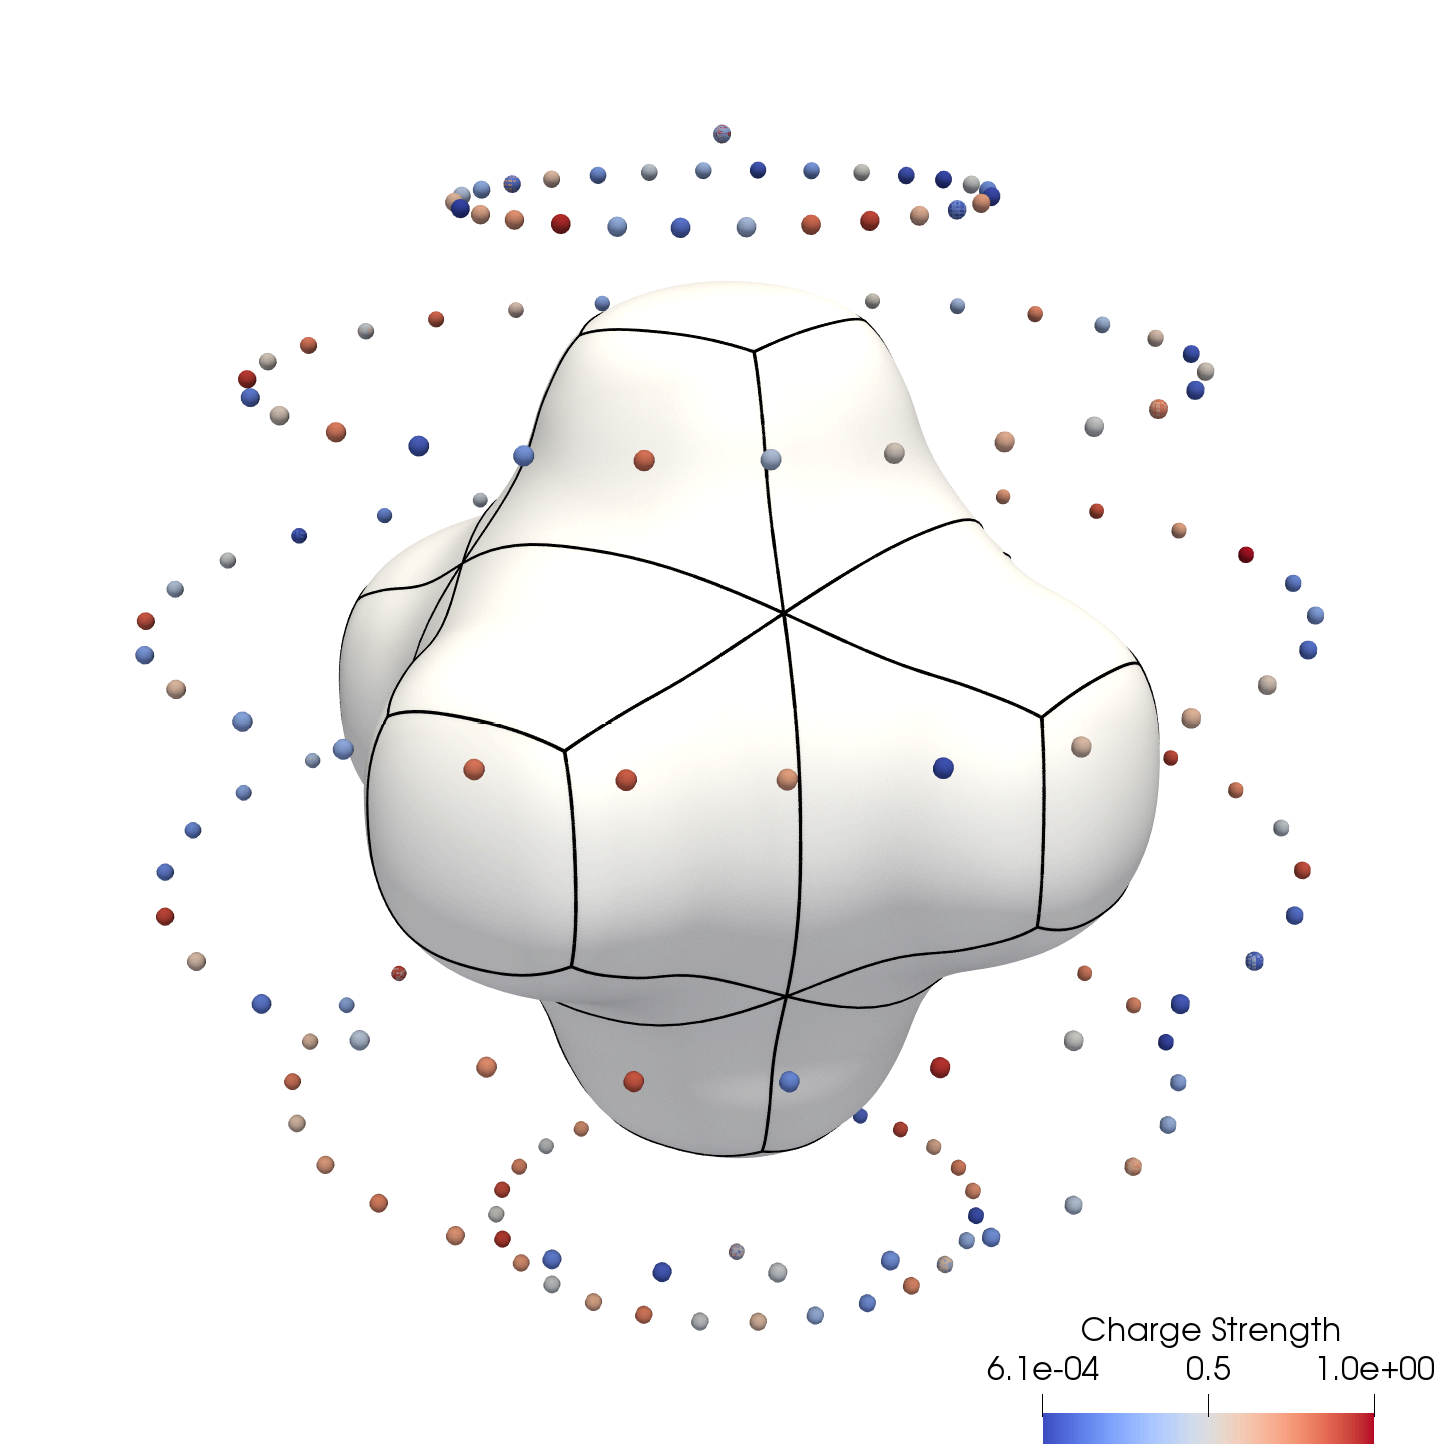
\includegraphics[width=.75\linewidth]{figs/pipe_convergence_setup}
  \end{minipage}\hfill
  \begin{minipage}{.5\textwidth}
      \centering
    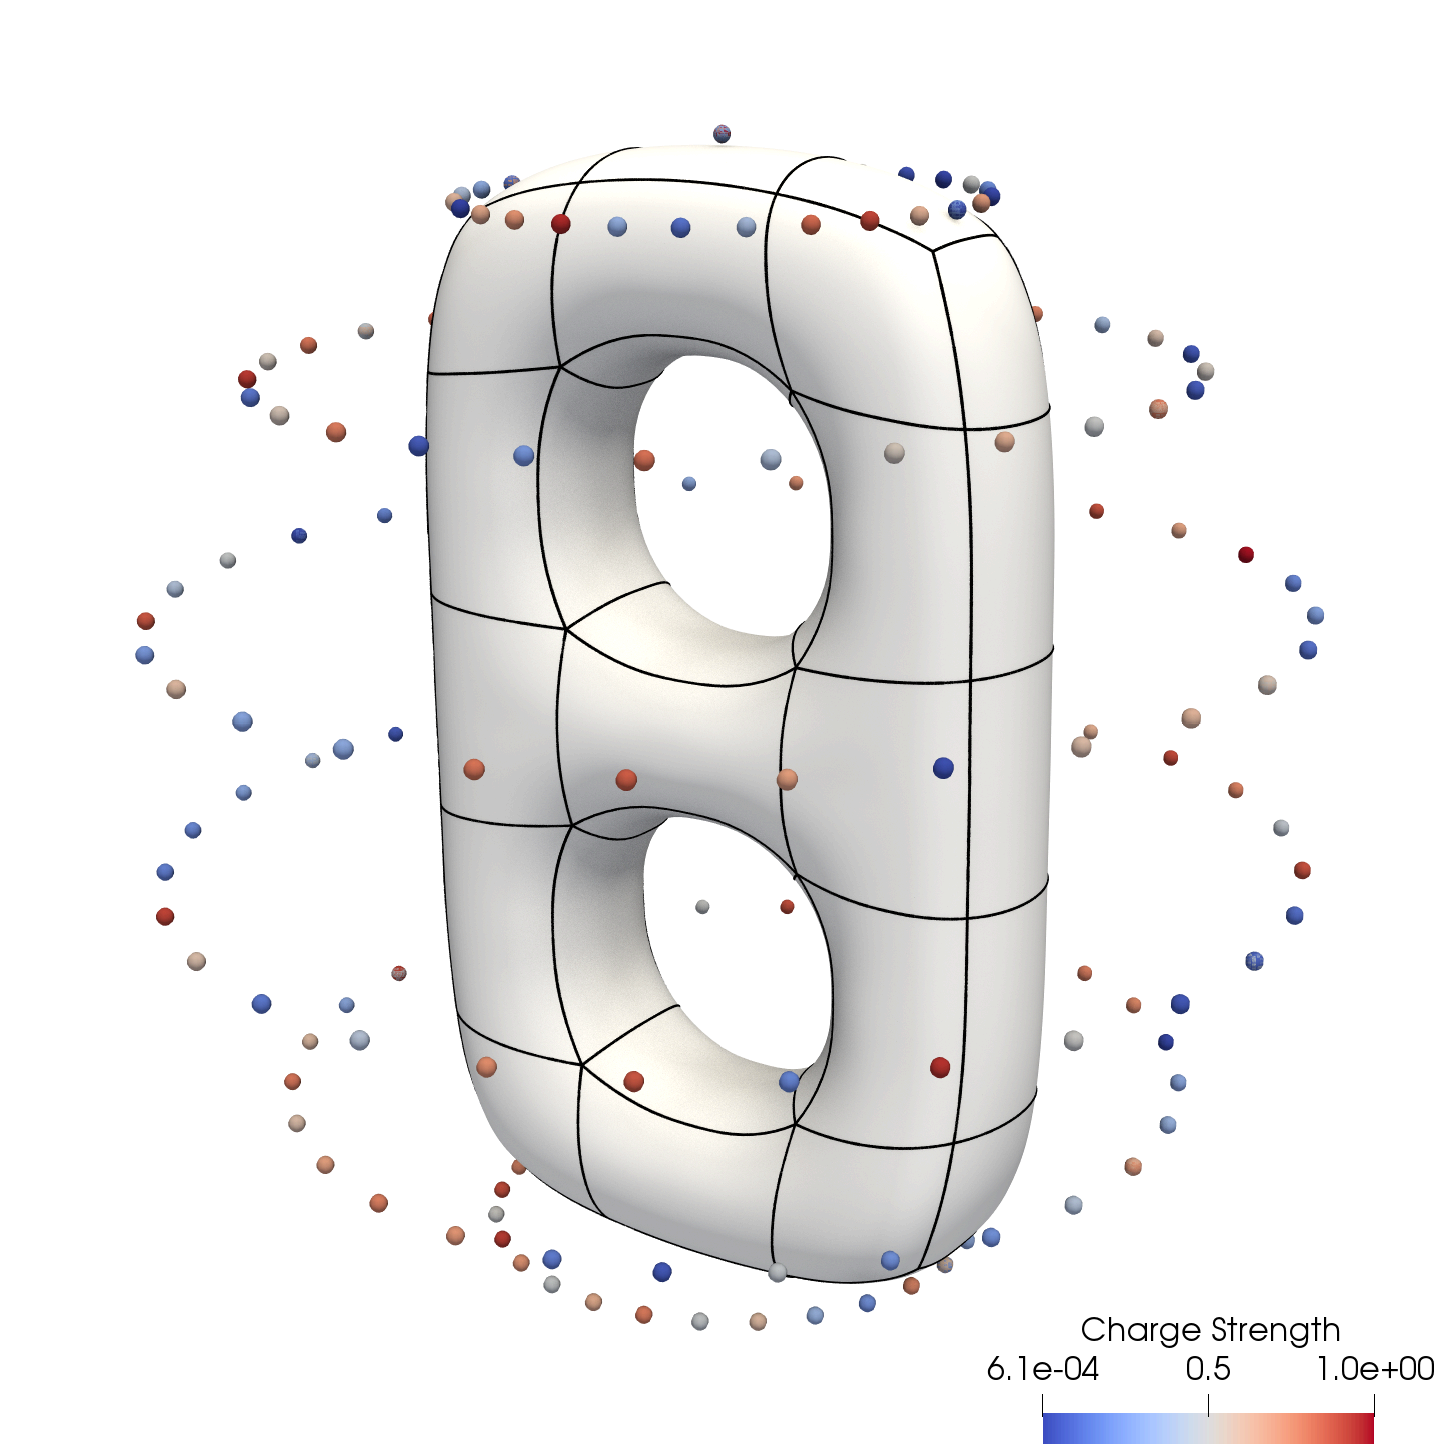
\includegraphics[width=.75\linewidth]{figs/ttorus2_convergence_setup}
  \end{minipage}\hfill
  \mcaption{fig:solver-conv-test-cases}{}{Geometry and singularities used for solver convergence tests. Figures are similar to \cref{fig:greens-id-test-cases}, but displaying geometries for testing the convergence of \qbkix within a \gmres solver.
  We use 30 16th-order polynomial patches for the pipe (left) and 50 20th-order patches for the genus two surface (right). 
  Note the proximity of the singularities to the domain of the genus two surface; the nearest singularity is less than $.05L$ from $\Gammah$.
}
\end{figure}

\begin{table}
\centering
\small
\setlength\tabcolsep{4pt}
\begin{tabular}{lllllll}
\toprule
{}Geometry & \pde &\multicolumn{4}{c}{Relative $\ell^\infty$ error (Number of patches)} & EOC\\
\midrule
Spheroid (\cref{fig:greens-id-test-cases}-left) & Laplace   &  $2.70\times 10^{-6 }$ (96) &  $1.92\times 10^{-7 }$ (384) &  $4.47\times 10^{-9 }$ (1536) &  $5.13\times 10^{-11 }$ (6144) & 5.35 \\
   \midrule
Pipe                                       & Laplace       &  $5.99\times 10^{-4 }$ (30) &  $3.03\times 10^{-5 }$ (120) &   $6.68\times 10^{-7 }$ (480) &  $2.27\times 10^{-8 }$ (1920) & 5.92\\
(\cref{fig:solver-conv-test-cases}-left)   & Elasticity    &  $7.17\times 10^{-2 }$ (30) &  $3.57\times 10^{-3 }$ (120) &   $8.90\times 10^{-5 }$ (480) &  $4.14\times 10^{-6 }$ (1920) & 5.45\\
                                           & Stokes        &  $8.53\times 10^{-2 }$ (30) &  $4.12\times 10^{-3 }$ (120) &   $1.03\times 10^{-4 }$ (480) &  $4.73\times 10^{-6 }$ (1920) & 5.43\\
   \midrule
Genus 2                                     & Laplace     &  $4.00\times 10^{-2 }$ (50) &  $1.25\times 10^{-4 }$ (200) &   $1.54\times 10^{-6 }$ (800) &  $5.73\times 10^{-10 }$ (3200) & 8.76 \\
(\cref{fig:solver-conv-test-cases}-right)   & Elasticity  &  $9.20\times 10^{-2 }$ (50) &  $1.05\times 10^{-3 }$ (200) &   $1.00\times 10^{-5 }$ (800) &  $9.44\times 10^{-8 }$ (3200) & 6.89\\
                                            & Stokes      &  $1.03\times 10^{-1 }$ (50) &  $1.18\times 10^{-3 }$ (200) &   $1.15\times 10^{-5 }$ (800) &  $1.03\times 10^{-7}$ (3200)& 6.88\\
\bottomrule
\end{tabular}
\mcaption{table:solver-data}{$\ell^\infty$ Relative error in \gmres solve and solution evaluation versus number of patches}{
  We solve \cref{eq:pde} by discretizing and evaluating the layer potential in the integral equation in \cref{eq:int-eq} as described in \cref{sec:singular-eval}.
  We use two-sided \qbkix inside of \gmres to solve for $\phi$, then evaluate \cref{eq:double_layer_disc} with one-sided \qbkix at a new set of points on $\Gammah$.
  Each column is the result of an additional level of uniform quadrisection of the patches in $\Pcoarse$. 
  The final column (EOC) is the estimated convergence order, computed via least-squares log-log fit of the error as a function of max patch size.
}
\end{table}

\begin{table}[!htb]
\centering
\small
\setlength\tabcolsep{8pt}
\begin{tabular}{llllll}
\toprule
{}Geometry & \pde &\multicolumn{4}{c}{Target points/second/core}\\
\midrule
%Cube                                    & Laplace         &  $2905$ &  $4124$ &  $4059$ &  $3979$ \\
Spheroid                                    & Laplace         &  $2737$ &  $3149$ &  $2846$ &  $2950$ \\
\midrule
%Pipe                                    & Laplace         &  $1894$ &  $3771$ &  $3757$ &  $4186$ \\
%(\cref{fig:greens-id-test-cases}-left)  & Elasticity      &  $361$  &  $451$ &   $459$  &  $480$  \\
%                                        & Stokes          &  $379$  &  $506$ &   $513$  &  $526$  \\
Pipe                                    & Laplace         &  $3046$ &  $2178$ &   $2832$  &  $2982$ \\
(\cref{fig:greens-id-test-cases}-left)  & Elasticity      &  $991$  &  $993$  &   $1189$  &  $1261$  \\
                                        & Stokes          &  $1048$ &  $1140$ &   $1335$  &  $1422$  \\
 \midrule
%Genus 2                                       & Laplace         &  $2542$  &  $3747$ &   $3895$  &  $4227$ \\
% (\cref{fig:greens-id-test-cases}-right)      & Elasticity      &  $350$  &  $531$ &   $553$  &  $564$ \\
%                                              & Stokes          &  $398$  & $587$ &   $638$  &  $X$ \\
Genus 2                                       & Laplace         &  $1862$ &  $2886$ &  $3122$  &  $2879$ \\
 (\cref{fig:greens-id-test-cases}-right)      & Elasticity      &  $729$  &  $1125$ &  $1255$  &  $1295$ \\
                                              & Stokes          &  $929$  &  $1304$ &  $1450$  &  $1504$ \\
\bottomrule
\end{tabular}
\mcaption{table:solver-perf-data}{Performance of singular evaluation in \gmres matrix-vector multiply}{
    For each test in \cref{table:solver-data}, we report the number of target points per second per core evaluated with two-sided \qbkix in a single \gmres matrix-vector multiplication.
}
\end{table}
We report the accuracy of the \qbkix scheme when used to solve \cref{eq:pde} via the integral equation in \cref{eq:int-eq}.
Two-sided \qbkix is used in the matrix-vector multiply inside \gmres to solve \cref{eq:int-eq} for the values of the density $\phi$ at the discretization points.
Then one-sided \qbkix is used to evaluate \cref{eq:double_layer_disc} at a slightly coarser discretization. 
Since \gmres minimizes the residual at the original discretization of \cref{eq:int-eq}, this final step prevents an artificially accurate solution by changing discretizations.
\cref{table:solver-data} lists the $\ell^\infty$ relative error values for the total solve and evaluation steps using \cref{sec:singular-eval} as we refine $\Pcoarse$ by subdivision as in the previous section.
In these tests, we choose $p=6$, $r= .005\sqrt{L}$ ($a = .005/\sqrt{L}$), and  $R= .03\sqrt{L}$ ($b = .03/\sqrt{L}$).
As for previous examples, we observe at least $5$th order convergence on all tested geometries in \cref{fig:solver-conv-test-cases} and \cref{fig:greens-id-test-cases}-left and all \pde's.
We include the spheroid example as an additional demonstration of a high accuracy solution via \gmres with our approach.
We report the number of target points evaluated per second per core with two-sided \qbkix in \cref{table:solver-perf-data}.
The results are similar to \cref{table:greens-id-perf-data}; the slower performance is because evaluation via two-sided \qbkix is more expensive than one-sided \qbkix.
\subsection{Comparison with \cite{YBZ}\label{sec:results-compare}}
In this section,  we compare our method to \cite{YBZ}, a previously proposed high-order, kernel-independent singular quadrature method in \threed for complex geometries. These characteristics are similar to  \qbkix shares these characteristics. \cite[Section 4]{morse2020bsupplementary} presents additional comparisons.

%To understand the performance of these two methods and see the implications of this complexity difference in practice, we now compare the performance of \qbkix with that of \cite{YBZ} on several concrete numerical examples.

The metric we are interested is \textit{cost for a given relative error}.
Assuming the surface discretization is $O(N)$, we measure the cost of a method as its total wall time during execution $T$ divided by the total wall time of an \fmm evaluation on the same $O(N)$ discretization, $T_\lbl{FMM}$. 
By normalizing by the \fmm evaluation cost, we minimize the dependence of the cost on machine- and implementation-dependent machine-dependent parameters.
%, such as clock speed, cache size, performance optimizations, etc.

We run the tests in this section on the spheroid geometry shown in \cref{fig:greens-id-test-cases}-left.
We focus on the singular quadrature scheme of \cite{YBZ}. 
The near-singular quadrature of \cite{YBZ} is algorithmically similar to \qbkix, but since an expensive singular quadrature rule is used as a part of near-singular evaluation, it has a higher total cost.
As a result, the accuracy and cost of near-singular evaluation of \cite{YBZ} is bounded by the accuracy and cost of the singular integration scheme.

To compare the full \qbkix method with \cite{YBZ}, we fit polynomial patches to the $C^\infty$ surface of \cite{ying2004simple}, denoted $\Gamma_b$, to produce $\Gammah$ during the first step of \cref{sec:admissible_algo}.
We apply the remaining geometry preprocessing algorithms of \cref{sec:admissible_algo} to $\Gammah$ to produce $\Pcoarse$.
After producing $\Pfine$ with two levels of uniform upsampling, we solve \cref{eq:int-eq} with two-sided \qbkix on $\Gammah$ and evaluate the solution on the boundary with one-sided \qbkix.
We then solve for the solution to \cref{eq:int-eq} on $\Gamma_b$ using \cite{YBZ}. 

For each of the tests in this section, we choose some initial spacing parameter
$h_0$ to discretize the surface of \cite{ying2004simple}, as in \cite{YBZ}, and use the $16\times$ upsampled grid and floating partition of unity radius proportional to $O(\sqrt{h})$, as in the original work.
We apply \qbkix to $\Gammah$ and the scheme of \cite{YBZ} to $\Gamma_b$ with spacing $h_0/2^i$, for $i=1,\hdots 4$.

As in the previous section, we choose the parameters $r$ and $R$ of \qbkix to be $O(\sqrt{L})$. 
For both quadrature methods, we use a multipole order of $16$ for \pvfmm with at most 250 points in each leaf box.
\begin{figure}[!htb]
  \centering
    \makebox[\textwidth][c]{ 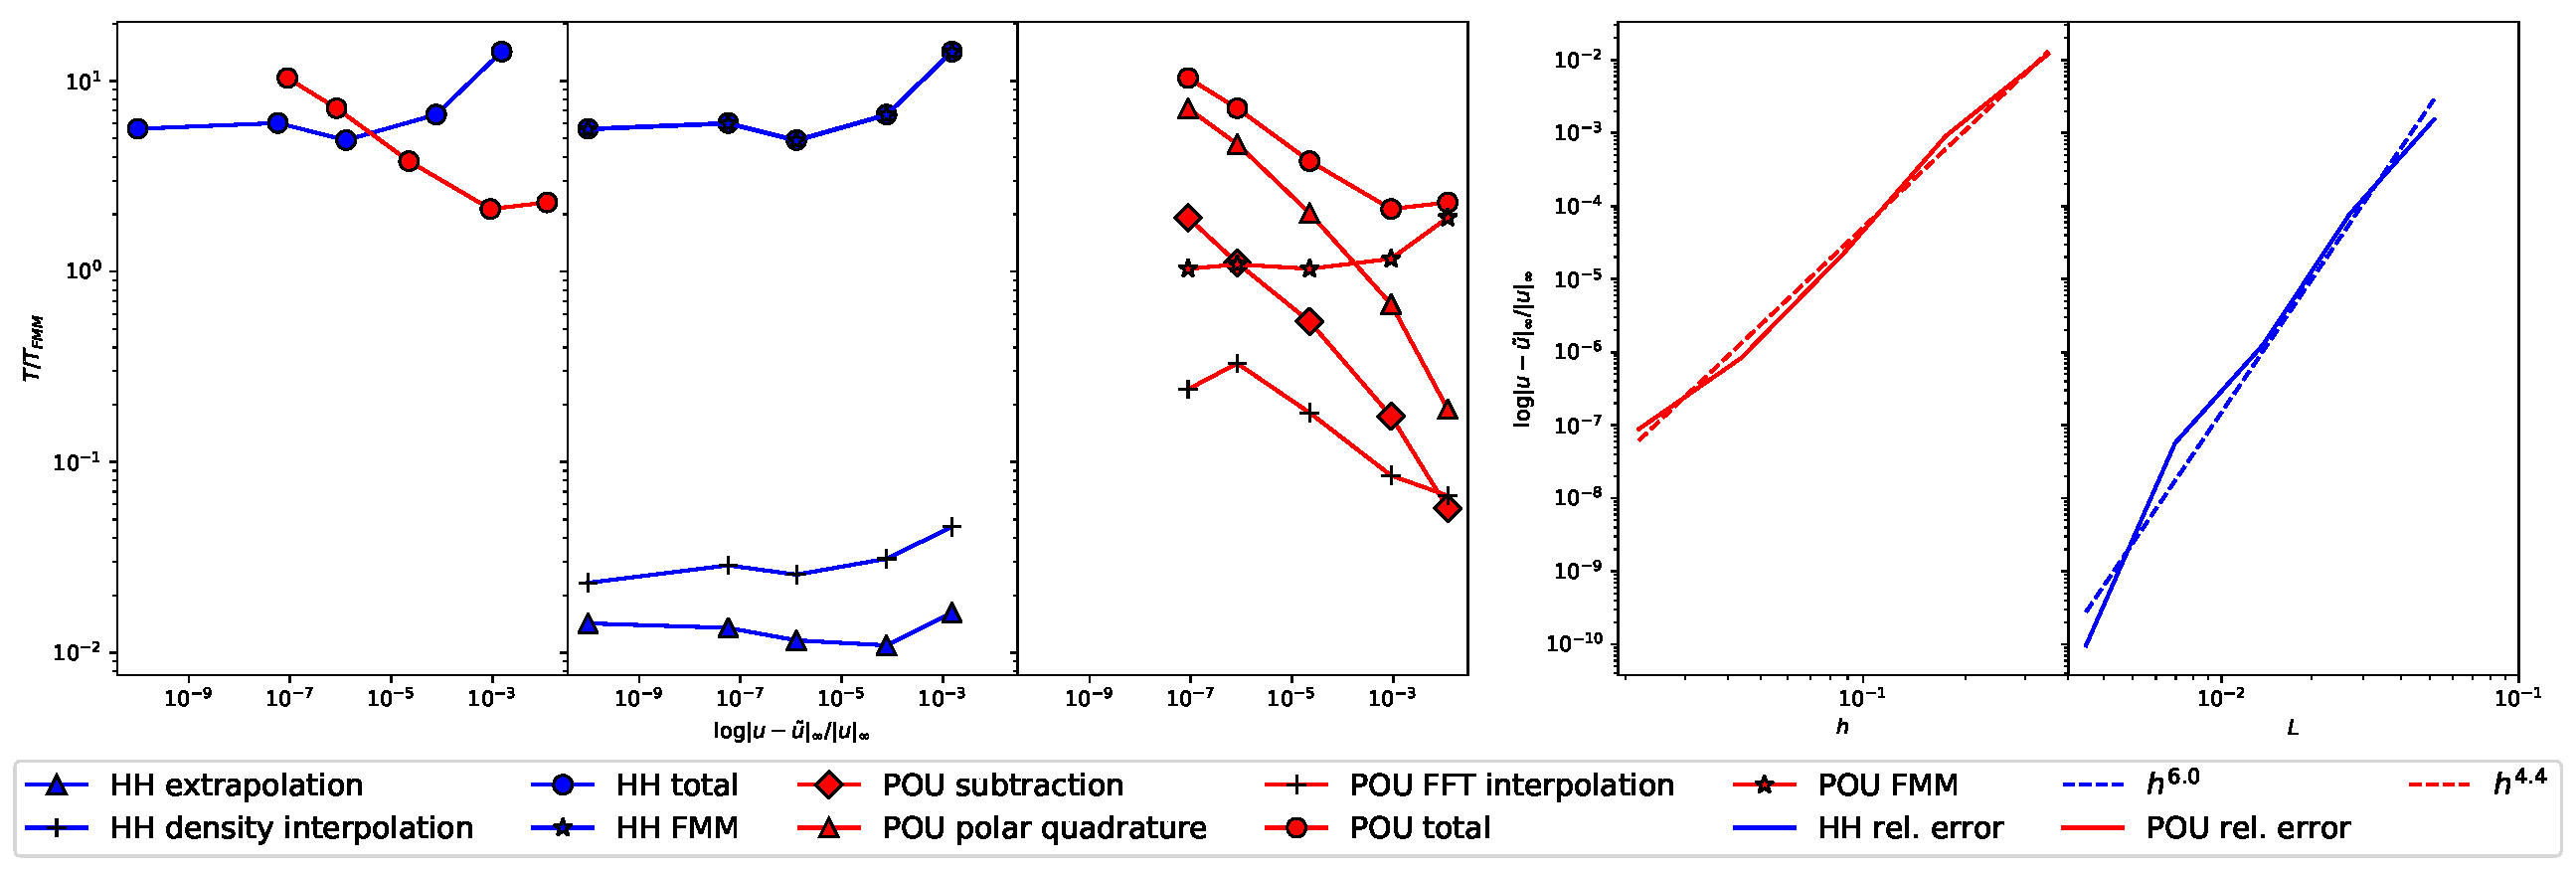
\includegraphics[width=1.1\textwidth]{figs/comparison_face_map_vs_blendsurf_cube_laplace_timing.pdf} }
    \makebox[\textwidth][c]{ 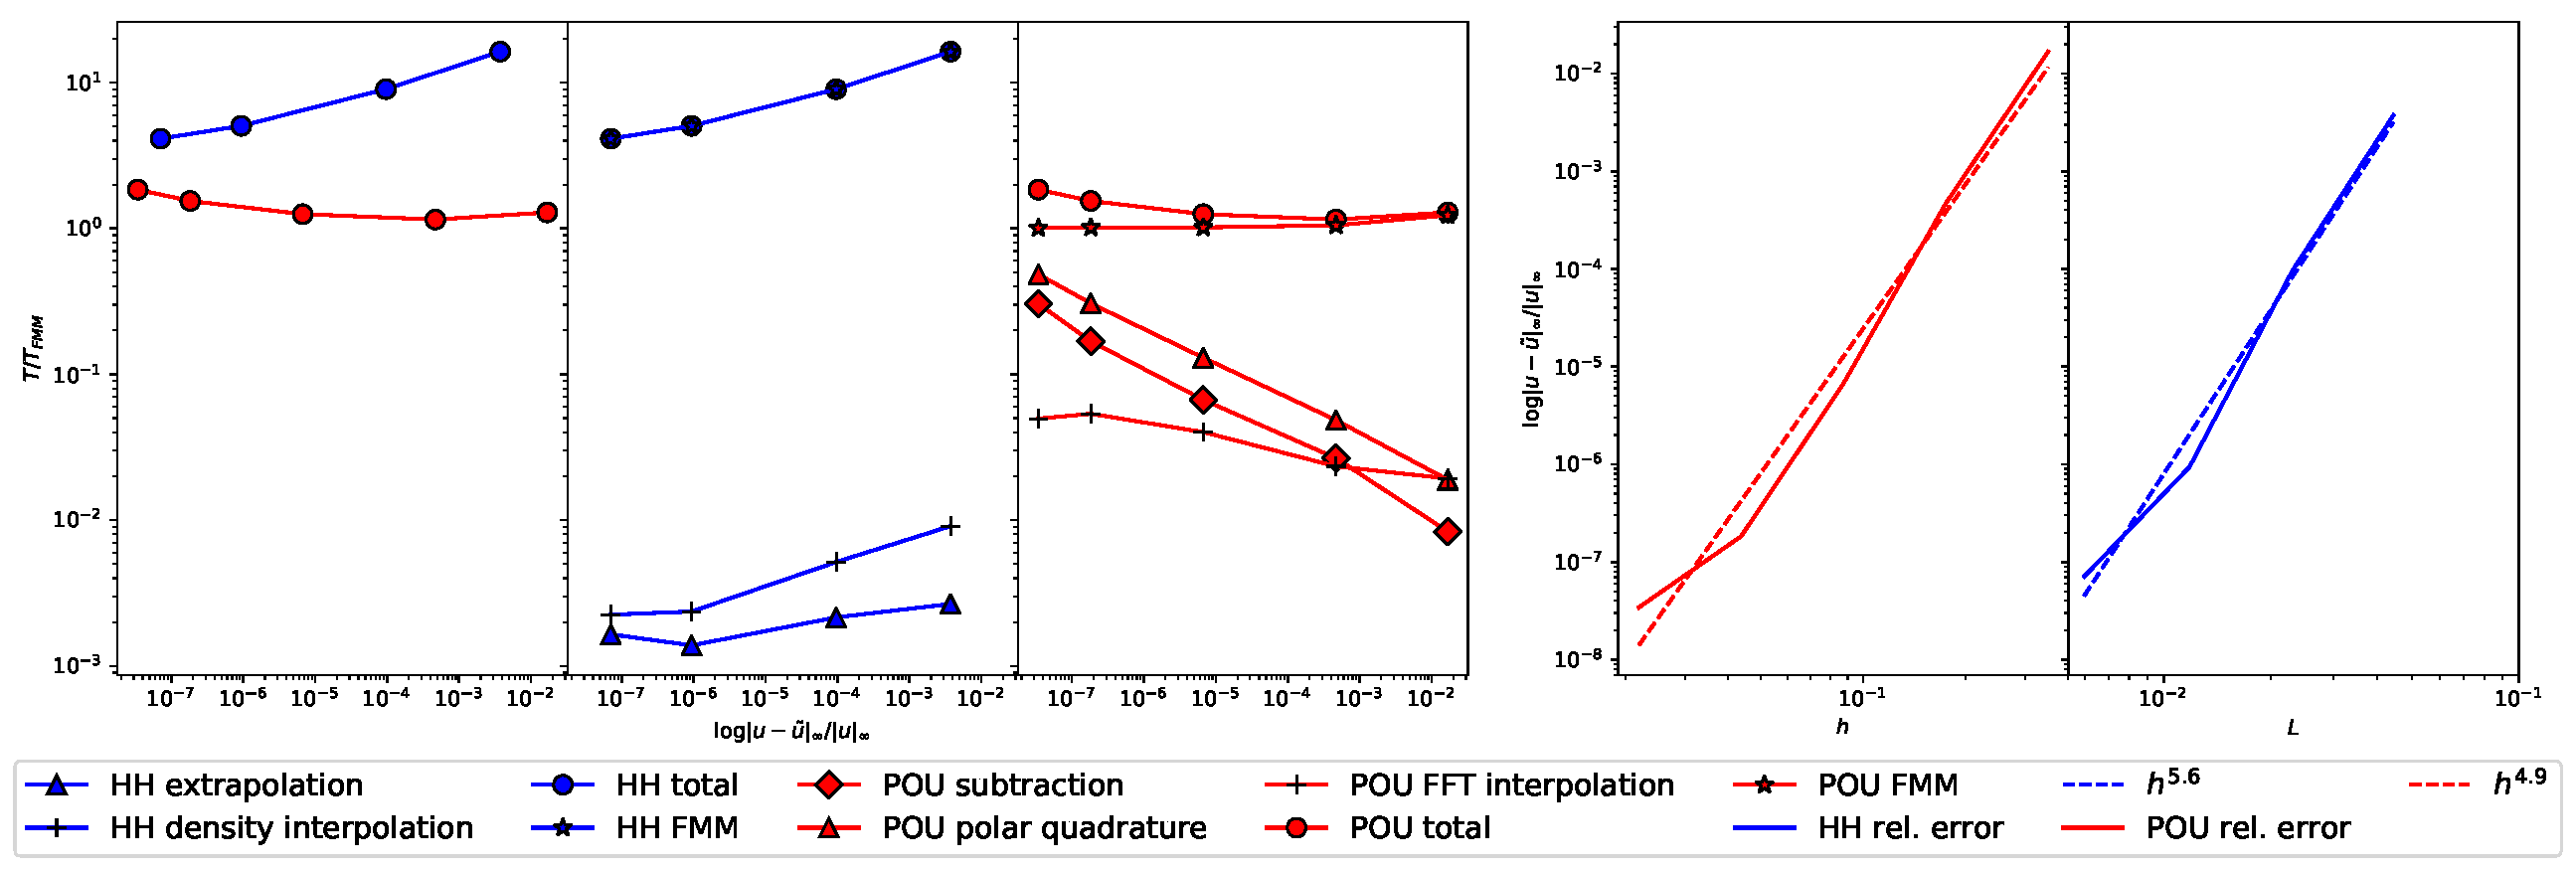
\includegraphics[width=1.1\textwidth]{figs/comparison_face_map_vs_blendsurf_cube_navier_timing.pdf} }
%  \hfill
%  \begin{minipage}{\textwidth}
%    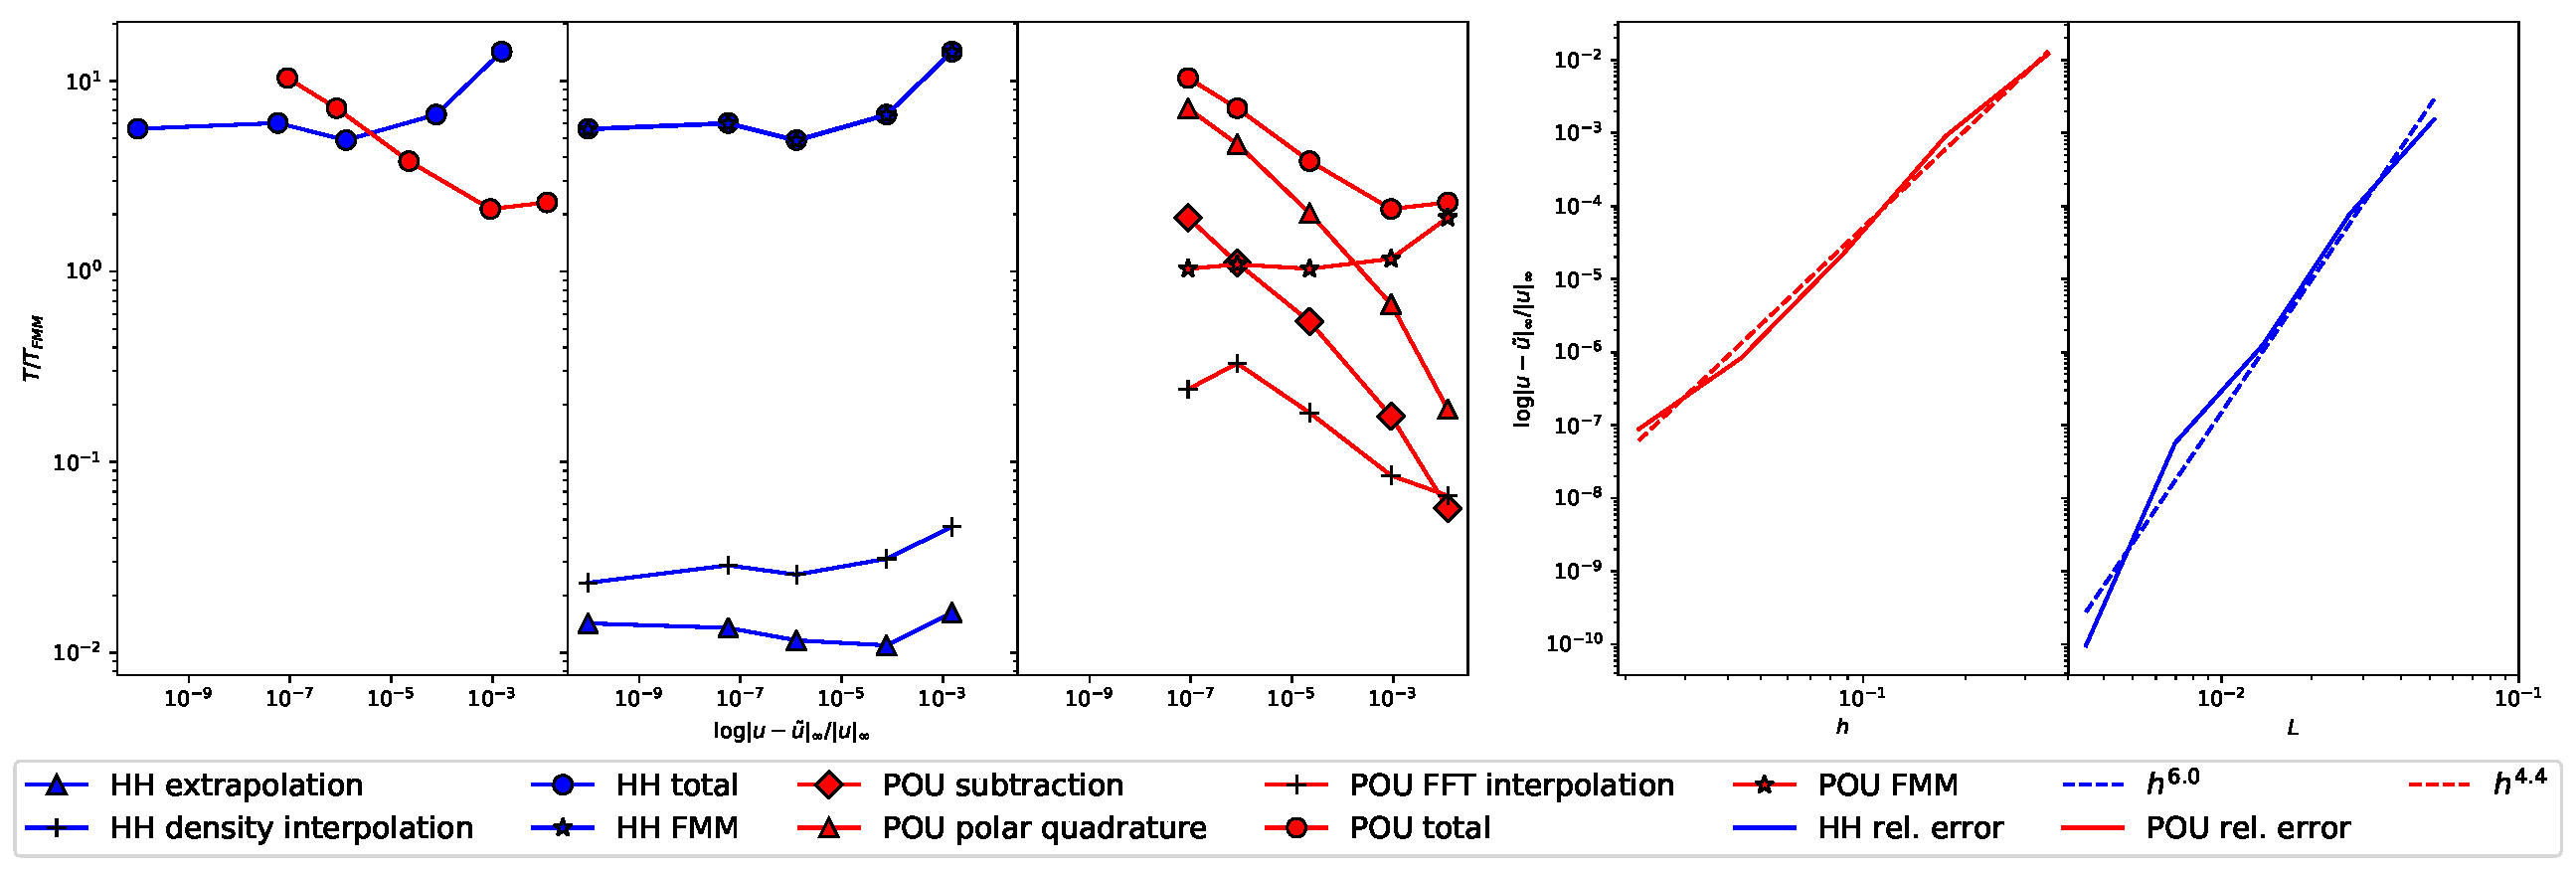
\includegraphics[width=\linewidth]{figs/comparison_face_map_vs_blendsurf_cube_laplace_timing.pdf}
%  \end{minipage}\hfill
%  \begin{minipage}{\textwidth}
%    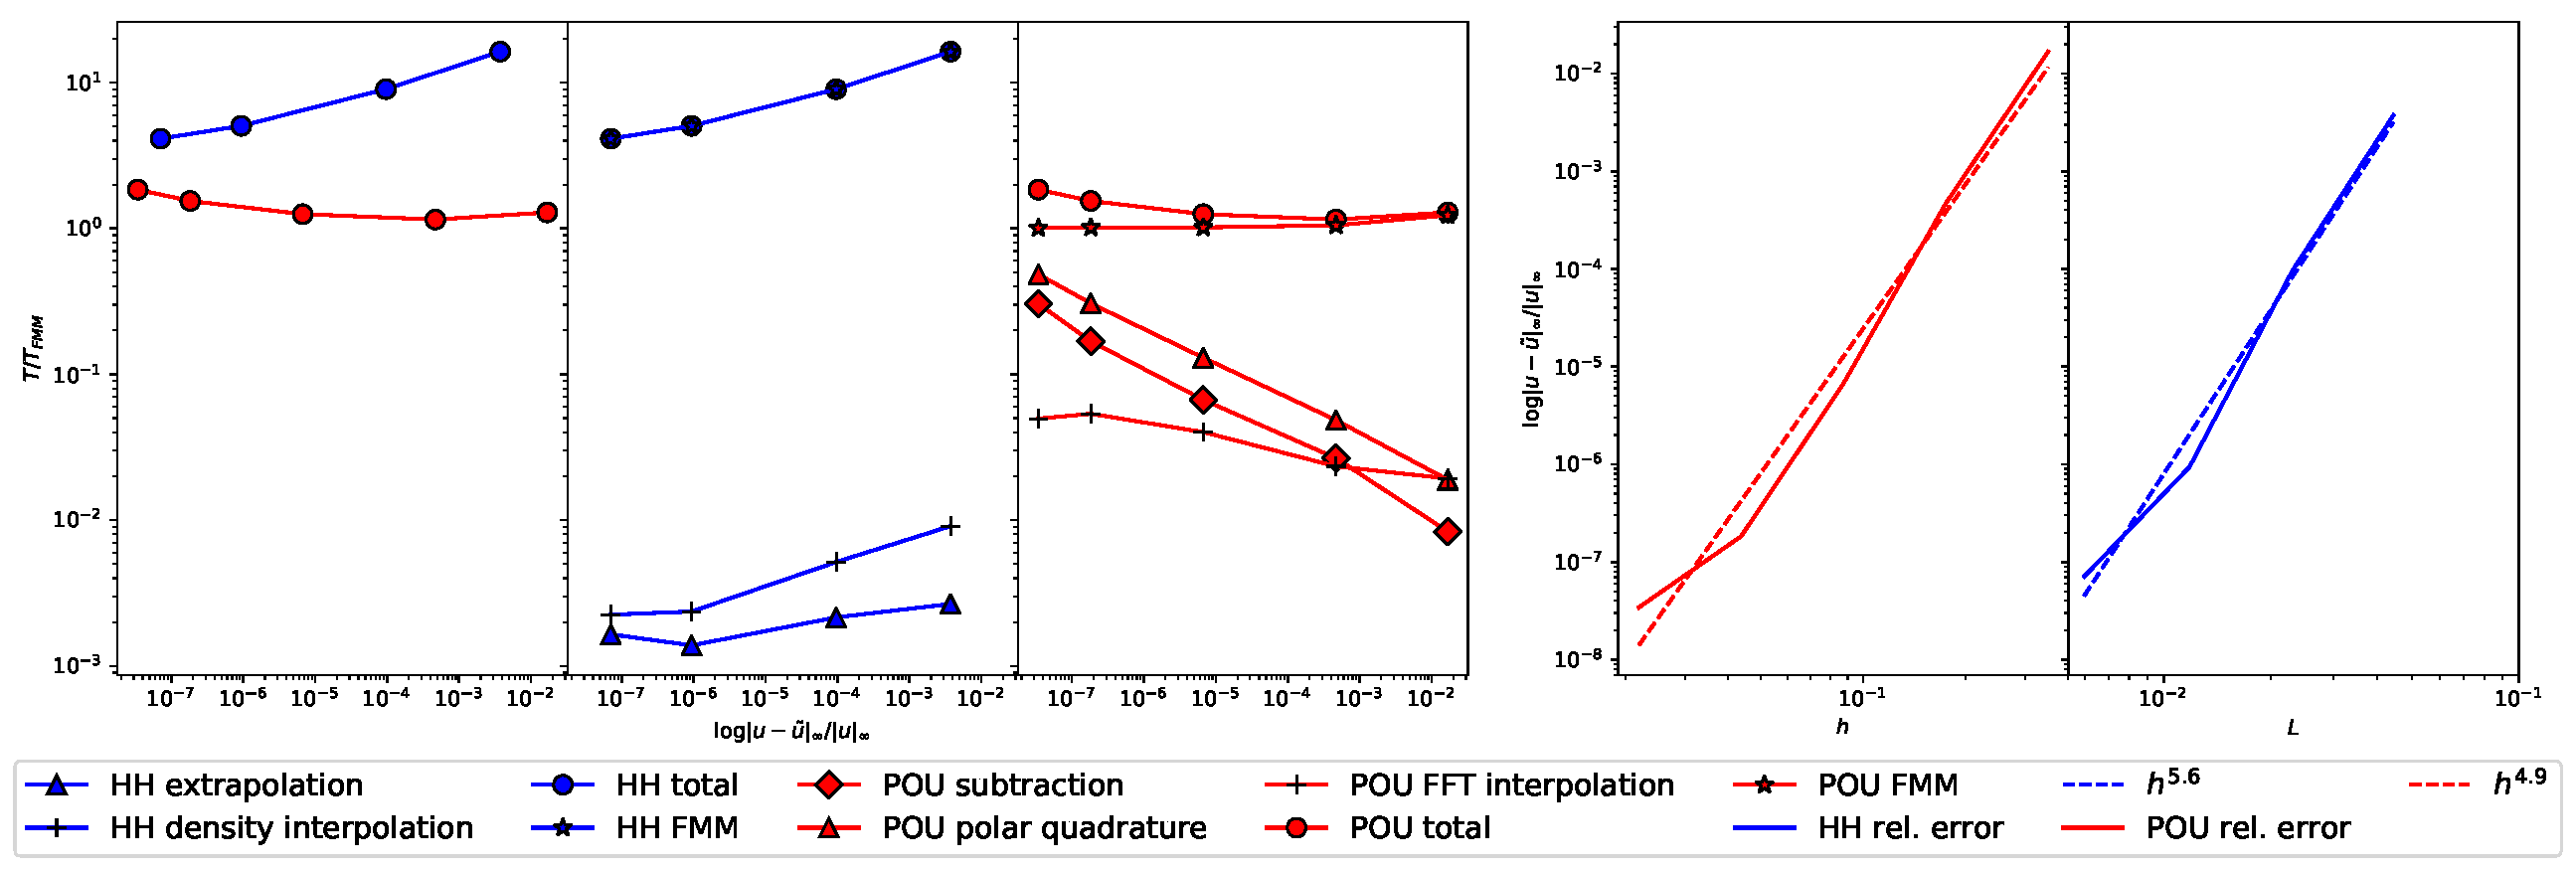
\includegraphics[width=\linewidth]{figs/comparison_face_map_vs_blendsurf_cube_navier_timing.pdf}
%  \end{minipage}\hfill
    \mcaption{fig:compare-solve-surface}{Comparison of \qbkix on polynomial patches (HH) versus \cite{YBZ} on the surface representation of \cite{ying2004simple} (POU) solving via \gmres for $u_c$}{
    Laplace (top) and elasticity (bottom) problems solved on the spheroid shown in \cref{fig:greens-id-test-cases}.
From left to right, we plot the total cost of each scheme, the cost of each subroutine for \qbkix (blue) and the singular quadrature scheme of \cite{YBZ} (red), and the relative error as a function of $h$.
    We plot error convergence of \cite{YBZ} as a function of $h$ and \qbkix as a function of $L$, due to the distinct discretizations.
    For \qbkix parameters, we choose $r=.013\sqrt{L}$, $R=.075\sqrt{L}$ for the Laplace problem; for the elasticity problem, we choose $r=.013\sqrt{L}$, $R=.08\sqrt{L}$. We choose $p=6$ and $q=15$ for both problems.
    For \cite{YBZ} the spacing is $h_0=.35$.
    Note that in the \qbkix timing breakdown, since the \fmm time is dominant, the \fmm cost lies directly on top of the total cost.
  }
\end{figure}
The results are shown in \cref{fig:compare-solve-surface}. 
From left to right, each plot details the total cost of each scheme, the cost of each subroutine for \qbkix (denoted \abbrev{HH}) and the singular quadrature scheme of \cite{YBZ} (denoted \abbrev{POU}), and the relative error as a function of $h$ and $L$, respectively, 
for all refinement levels. 
%Each data point in the plots, from right to left, is the result of $4\times $ finer sampling of the surfaces.
We plot the cost of both schemes the cost of each algorithmic step as a function of their computed relative error. 
In each figure, we present results for a Laplace problem (top) and an elasticity problem (bottom). % to highlight the difference in performance between scalar and vector kernels.

In \cref{fig:compare-solve-surface}, as expected, we observe a  higher  convergence rate for \qbkix compared to \cite{YBZ}. 
\cite{YBZ} outperforms \qbkix in terms of cost for all tested discretizations.  
%\DZ{For vector problems, the cost of additional \qbkix evaluations 
%for the problem size considered outweighs the savings from not using an asymptotically 
%more expensive singular quadrature.}
% This is due to the greater cost of a vector \fmm evaluation compared to a scalar one: the $m+p$  \fmm evaluation of \cite{YBZ} can be accelerated more efficiently with the method's small dense linear algebra computations.
 We observe that the \fmm evaluation in \cref{fig:compare-solve-surface} accounts for at least 95\% of the \qbkix cost.
This means that a local singular quadrature method (based on corrections to an \fmm evaluation, \cref{sec:related_work}) of \textit{worse} complexity can beat a global method, simply by virtue of reducing the \fmm size.
%Moreover, our implementation of \cite{YBZ} is not highly optimized, so we can expect a well-engineered \pou singular quadrature implementation such as \cite{malhotra2019taylor} to widen this gap.
By noting the large difference between the \qbkix \fmm cost and the \qbkix density interpolation, we can reasonably infer that a local \qbkix scheme should narrow this  performance gap and outperform \cite{YBZ} for larger problems, assuming that switching to a local scheme does not dramatically affect error convergence. 

%\qbkix is more efficient in the high-accuracy regime for Laplace problems, but \cite{YBZ} is more efficient for low-accuracy Laplace and elasticity problems.
%However, main difference from the previous section is that the crossover point in performance appears to be larger; \qbkix becomes more efficient than \cite{YBZ} around $10^{-5}$ and the gap between \qbkix and \cite{YBZ} for elasticity is less dramatic at $10^{-8}$.
%We attribute this improvement to the more efficient Clenshaw-Curtis discretization of \qbkix compared to the overlapping trapezoidal discretization of \cite{YBZ}.
%This is further supporting evidence that a local \qbkix implementation should surpass \cite{YBZ}.

\subsection{Requested target precision vs. computed accuracy}
\begin{figure}[!htb]
\begin{tikzpicture}
    \begin{loglogaxis}[
        xlabel=$\err{target}$,
        ylabel= $\infty$-norm relative error,
        ylabel near ticks,
        xlabel near ticks,
        label style={font=\scriptsize},
        tick label style={font=\scriptsize},
        width=.333\linewidth%7cm,height=3cm
    ]
    \addplot[smooth,mark=*,blue] plot coordinates {
        (1e-4,0.0003143683435301948)
        (1e-5,6.031924968205908e-05)
        (1e-6,4.103514547039301e-06)
        (1e-7,6.614064613404895e-07)
        (1e-8,1.122384348756594e-07)
    };
        \addplot[domain=1e-8:1e-4,dotted,thick]{x};

    \end{loglogaxis}
    \end{tikzpicture}
    \begin{tikzpicture}
    \begin{semilogxaxis}[
        xlabel=$\err{target}$,
        ylabel= Target points/second/core,
        ylabel near ticks,
        xlabel near ticks,
        label style={font=\scriptsize},
        tick label style={font=\scriptsize},
        width=.333\linewidth%7cm,height=3cm
    ]
    \addplot[smooth,mark=*,blue] plot coordinates {
        (1e-4,2077)
        (1e-5,1620)
        (1e-6,772)
        (1e-7,400)
        (1e-8,222)
    };
    \end{semilogxaxis}
    \end{tikzpicture}
    \begin{tikzpicture}
    \begin{loglogaxis}[
        xlabel=$\err{target}$,
        ylabel= Number of patches,
        ylabel near ticks,
        xlabel near ticks,
        label style={font=\scriptsize},
        tick label style={font=\scriptsize},
        legend style={font=\tiny},
         legend image post style={scale=0.5},
        width=.333\linewidth%7cm,height=3cm
    ]
    \addplot[smooth,mark=*,blue] plot coordinates {
        (1e-4,128)
        (1e-5,128)
        (1e-6,128)
        (1e-7,128)
        (1e-8,128)
    };
    \addlegendentry{$|\Pcoarse|$}
    \addplot[smooth,mark=*,red] plot coordinates {
        (1e-4,5408)
        (1e-5,8288)
        (1e-6,28256)
        (1e-7,60032)
        (1e-8,113936)
    };
    \addlegendentry{$|\Pfine|$}
    \end{loglogaxis}
    \end{tikzpicture}
        \mcaption{fig:full-algo-perf}{Performance of full algorithm}{
            Left: $\infty$-norm relative error in singular integral vs requested target accuracy (blue). 
        The dotted line is the ideal behavior $y=x$.
        Middle: Performance in terms of target points evaluated per second per core with \qbkix.
        Right: Number of patches in $\Pcoarse$ and $\Pfine$ computed by the preprocessing algorithms.}
\end{figure}

In this section, we study the performance of the full algorithm outlined in \cref{sec:algo}.
We test \qbkix on the torus domain shown in \cref{fig:greens-id-test-cases}-right.
We choose a reference solution of the form of \cref{eq:point-charge-solution} with a single point charge located at the origin, in the middle of the hole of the torus.
We solve the integral equation with two-sided \qbkix and evaluate the singular integral on a distinct discretization with one-sided \qbkix.
We choose $q=20$, $p=6$ and $a=b/6$.
We select various values for $\err{target}$ using the plot in \cref{fig:extrap-err-p6} to choose $b$ to ensure sufficiently accurate extrapolation. 
We plot the results of our tests in \cref{fig:full-algo-perf}.

We see in \cref{fig:full-algo-perf}-left that we are consistently close to the requested target precision. 
We see a decline in target points per second per core as accuracy increases in \cref{fig:full-algo-perf}-middle.
This is explained by \cref{fig:full-algo-perf}-right, which shows an increase in the size $\Pfine$ as $\Pcoarse$ remains a fixed size.
The initial 128 patches in $\Pcoarse$ are enough to resolve the boundary condition and $\Gamma$, but we need greater quadrature accuracy for lower values of $\err{target}$ .
Decreasing the number of points in passed to the \fmm, i.e., decreasing the size of $\Pfine$, is the main way to improve performance of our method.
This is further indication that a local version of \qbkix will outperform a global approach.

\subsection{Full algorithm on interlocking torii\label{sec:results-torii}}
We now demonstrate the full algorithm pipeline on an exterior Laplace problem, whose boundary is defined by four interlocking torii shown in \cref{fig:torii}.
The domain boundary is contained in the box $[-3.8, 2.4] \times [-1.1, 1.1] \times [-1,1]$.
The shortest distance between two adjacent torii is less than 10\% of a polynomial patch length defining the boundary.
We again use a boundary condition of the form \cref{eq:point-charge-solution} with a single point charge located at $(0,.03,.875)$, inside the upper half of the second torus from the right in \cref{fig:torii}.
This problem is challenging due to the nearly touching geometry of the torii, along with the singularity placed close to the boundary.
We run the admissibility and adaptive upsampling algorithms outlined in \cref{sec:algo}, solve \cref{eq:int-eq} using two-sided \qbkix, and evaluate the solution on the boundary using one-sided \qbkix.
The absolute error in the $\infty$-norm of the singular evaluation is plotted on the boundary surface.

\begin{figure}[!htb]
  \centering
  \hfill
  \begin{minipage}{.65\textwidth}
    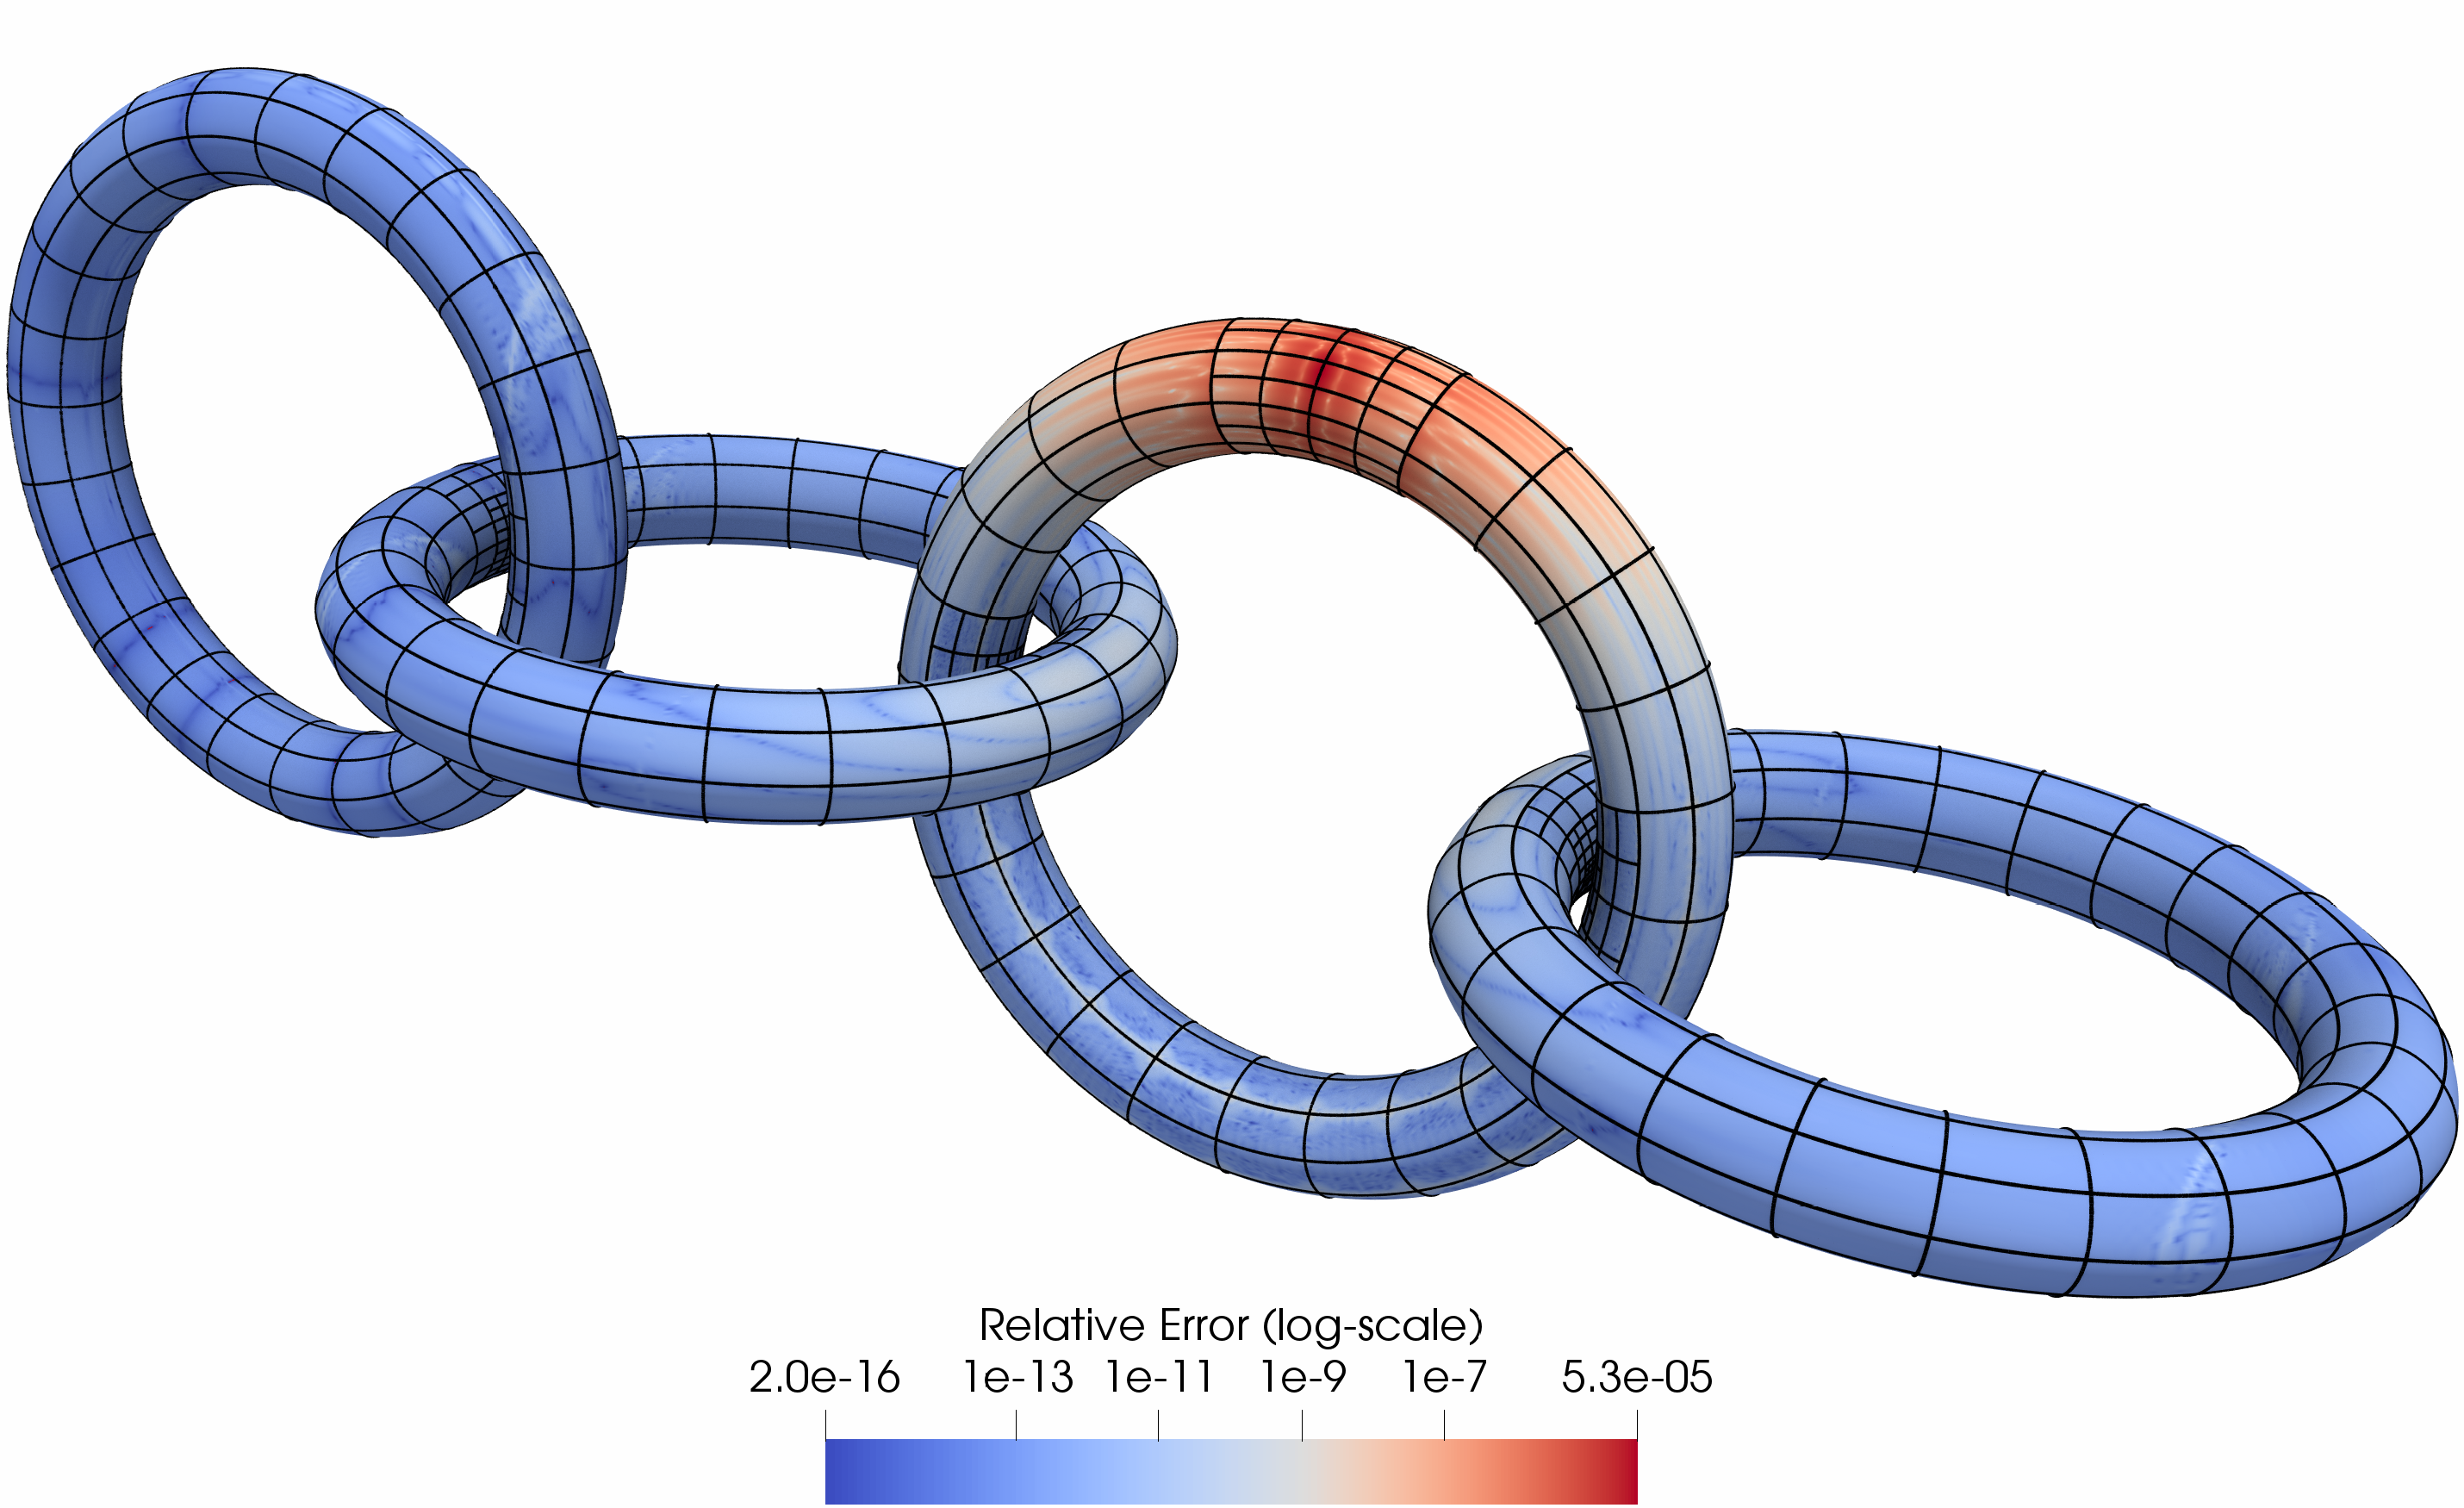
\includegraphics[width=\linewidth]{figs/interlocking_torus_error.png}
  \end{minipage}\hfill
  \begin{minipage}{.35\textwidth}
    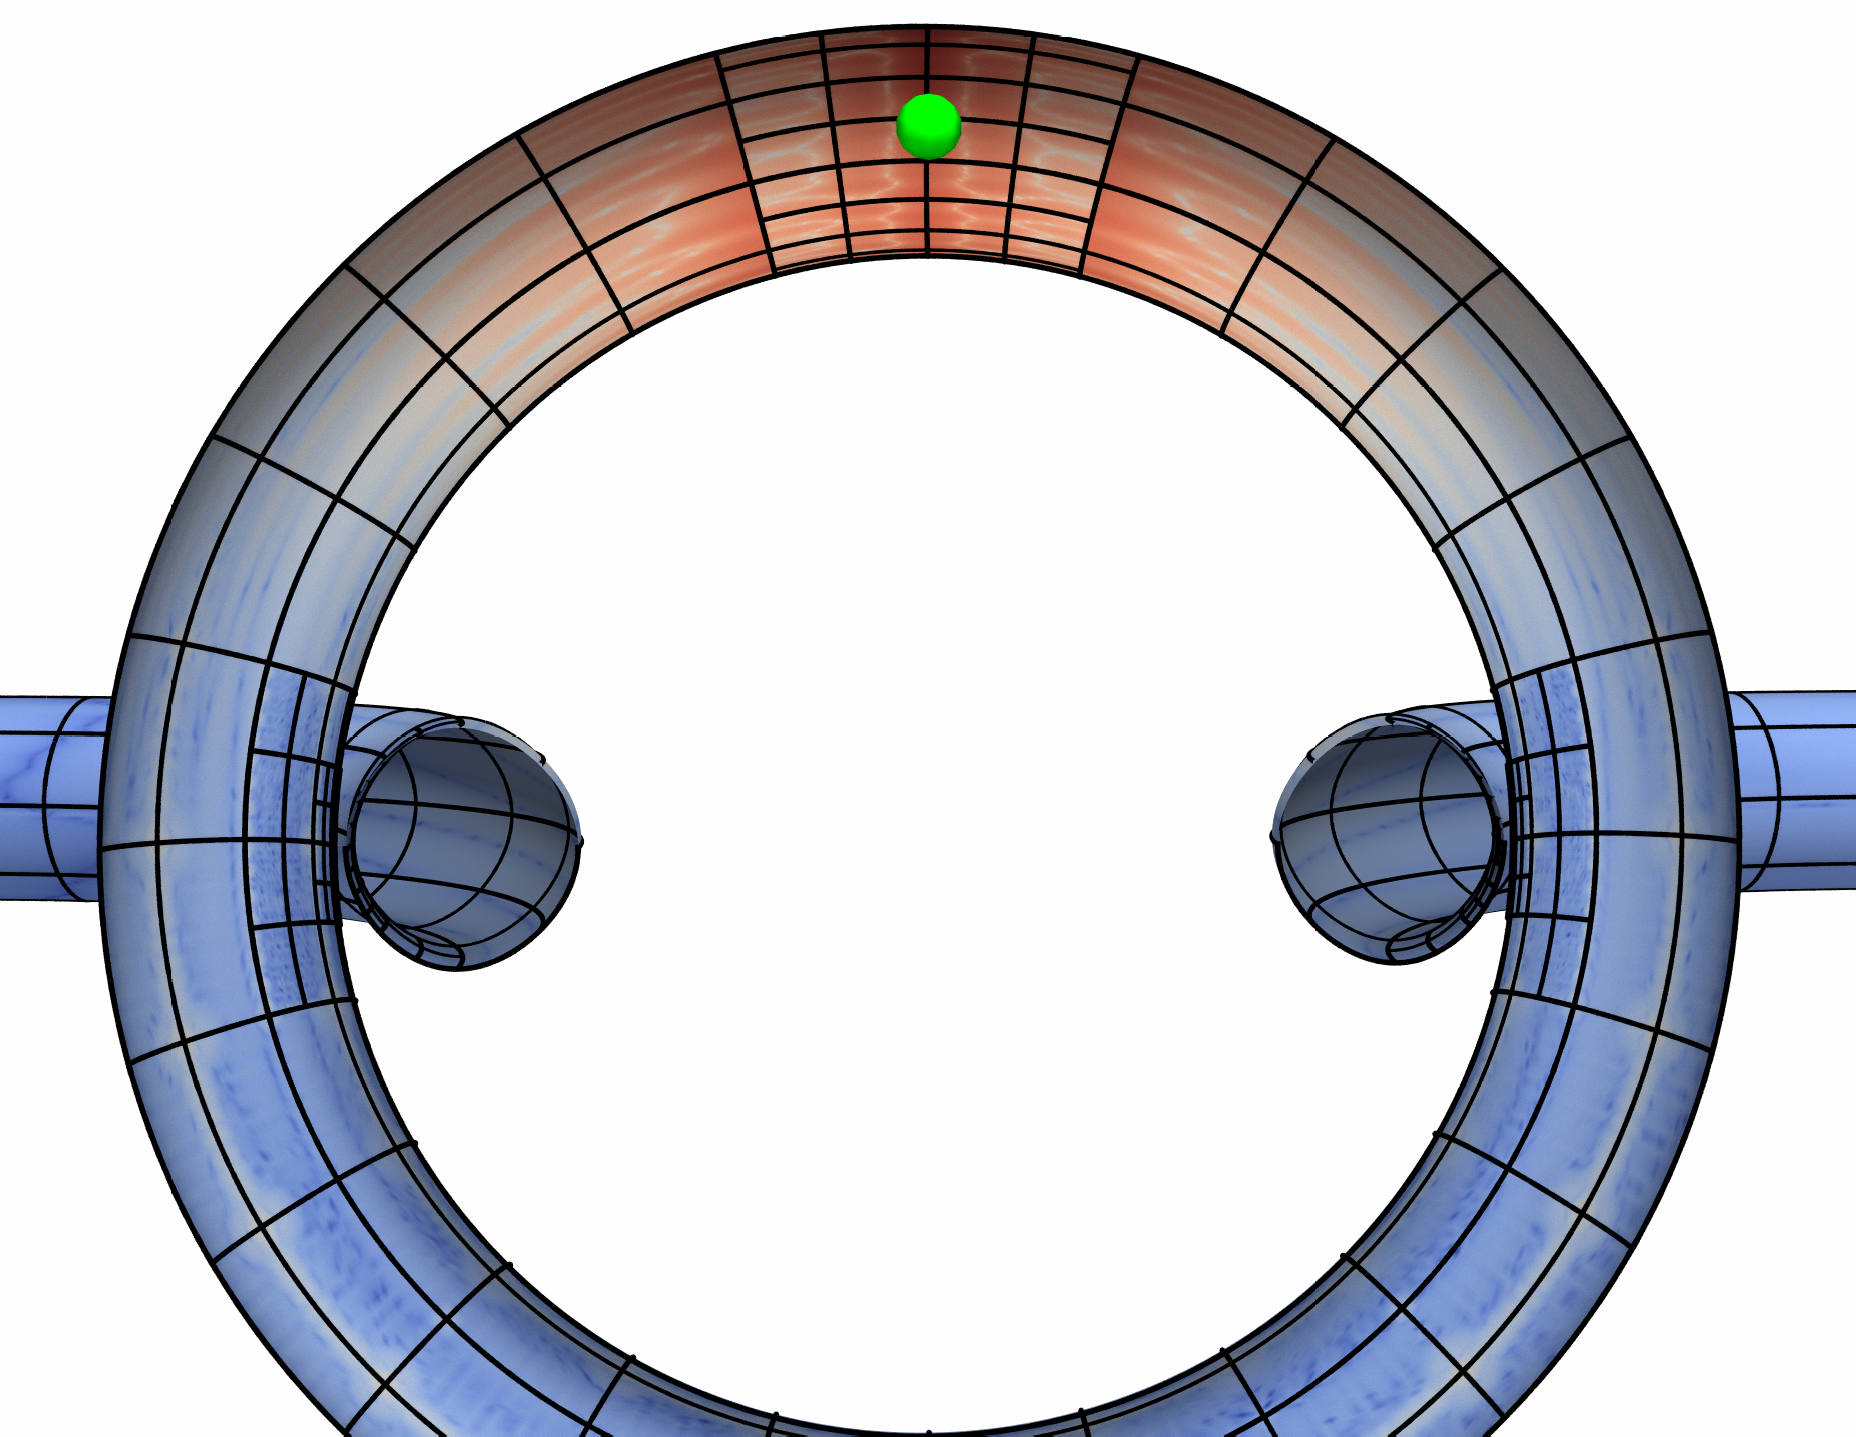
\includegraphics[width=\linewidth]{figs/interlocking_torus_error_cross_section.png}
  \end{minipage}\hfill
  \mcaption{fig:torii}{Absolute error of \gmres solve via \qbkix on interlocking torii}{Left: The admissible set of 1128 patches in $\Pcoarse$ used to solve \cref{eq:int-eq} is shown (black lines denote patch boundaries).
  The point charge generated the boundary condition is located within the second torus from the right. 
    Right: a cross-section of the torii geometry through the $xz$-plane, showing the second torus from the right and the location of the singularity (green point).
}
\end{figure}
Using $a=.1$, $b=.025$, $p=6$ and $q=20$, we achieve a maximum pointwise error of $1.29\times 10^{-5}$. 
\gmres was able to reduce the residual by a factor of $10^{-13}$ over 109 iterations.
There are 288768 quadrature points in the coarse discretization, 18235392 quadrature points in the fine discretization, and 3465216 check points used in the two-sided \qbkix evaluation inside \gmres.
We evaluate the solved density at 451200 points on the boundary with one-sided \qbkix to produce the render in \cref{fig:torii}.
On a machine with two Intel Xeon E-2690v2 3.0GHz \abbrev{CPU}'s, each with 10 cores, and 100 \abbrev{GB} of \abbrev{RAM},
the \gmres solve and interior evaluation required 5.7 hours and can evaluate the singular integral at a rate of 1709 target points per second per core.


\subsection{Solution on complex geometry\label{sec:results-blood-vessel}}

\begin{figure}[!htb]
  \centering
  \hfill
  \begin{minipage}{.7\textwidth}
    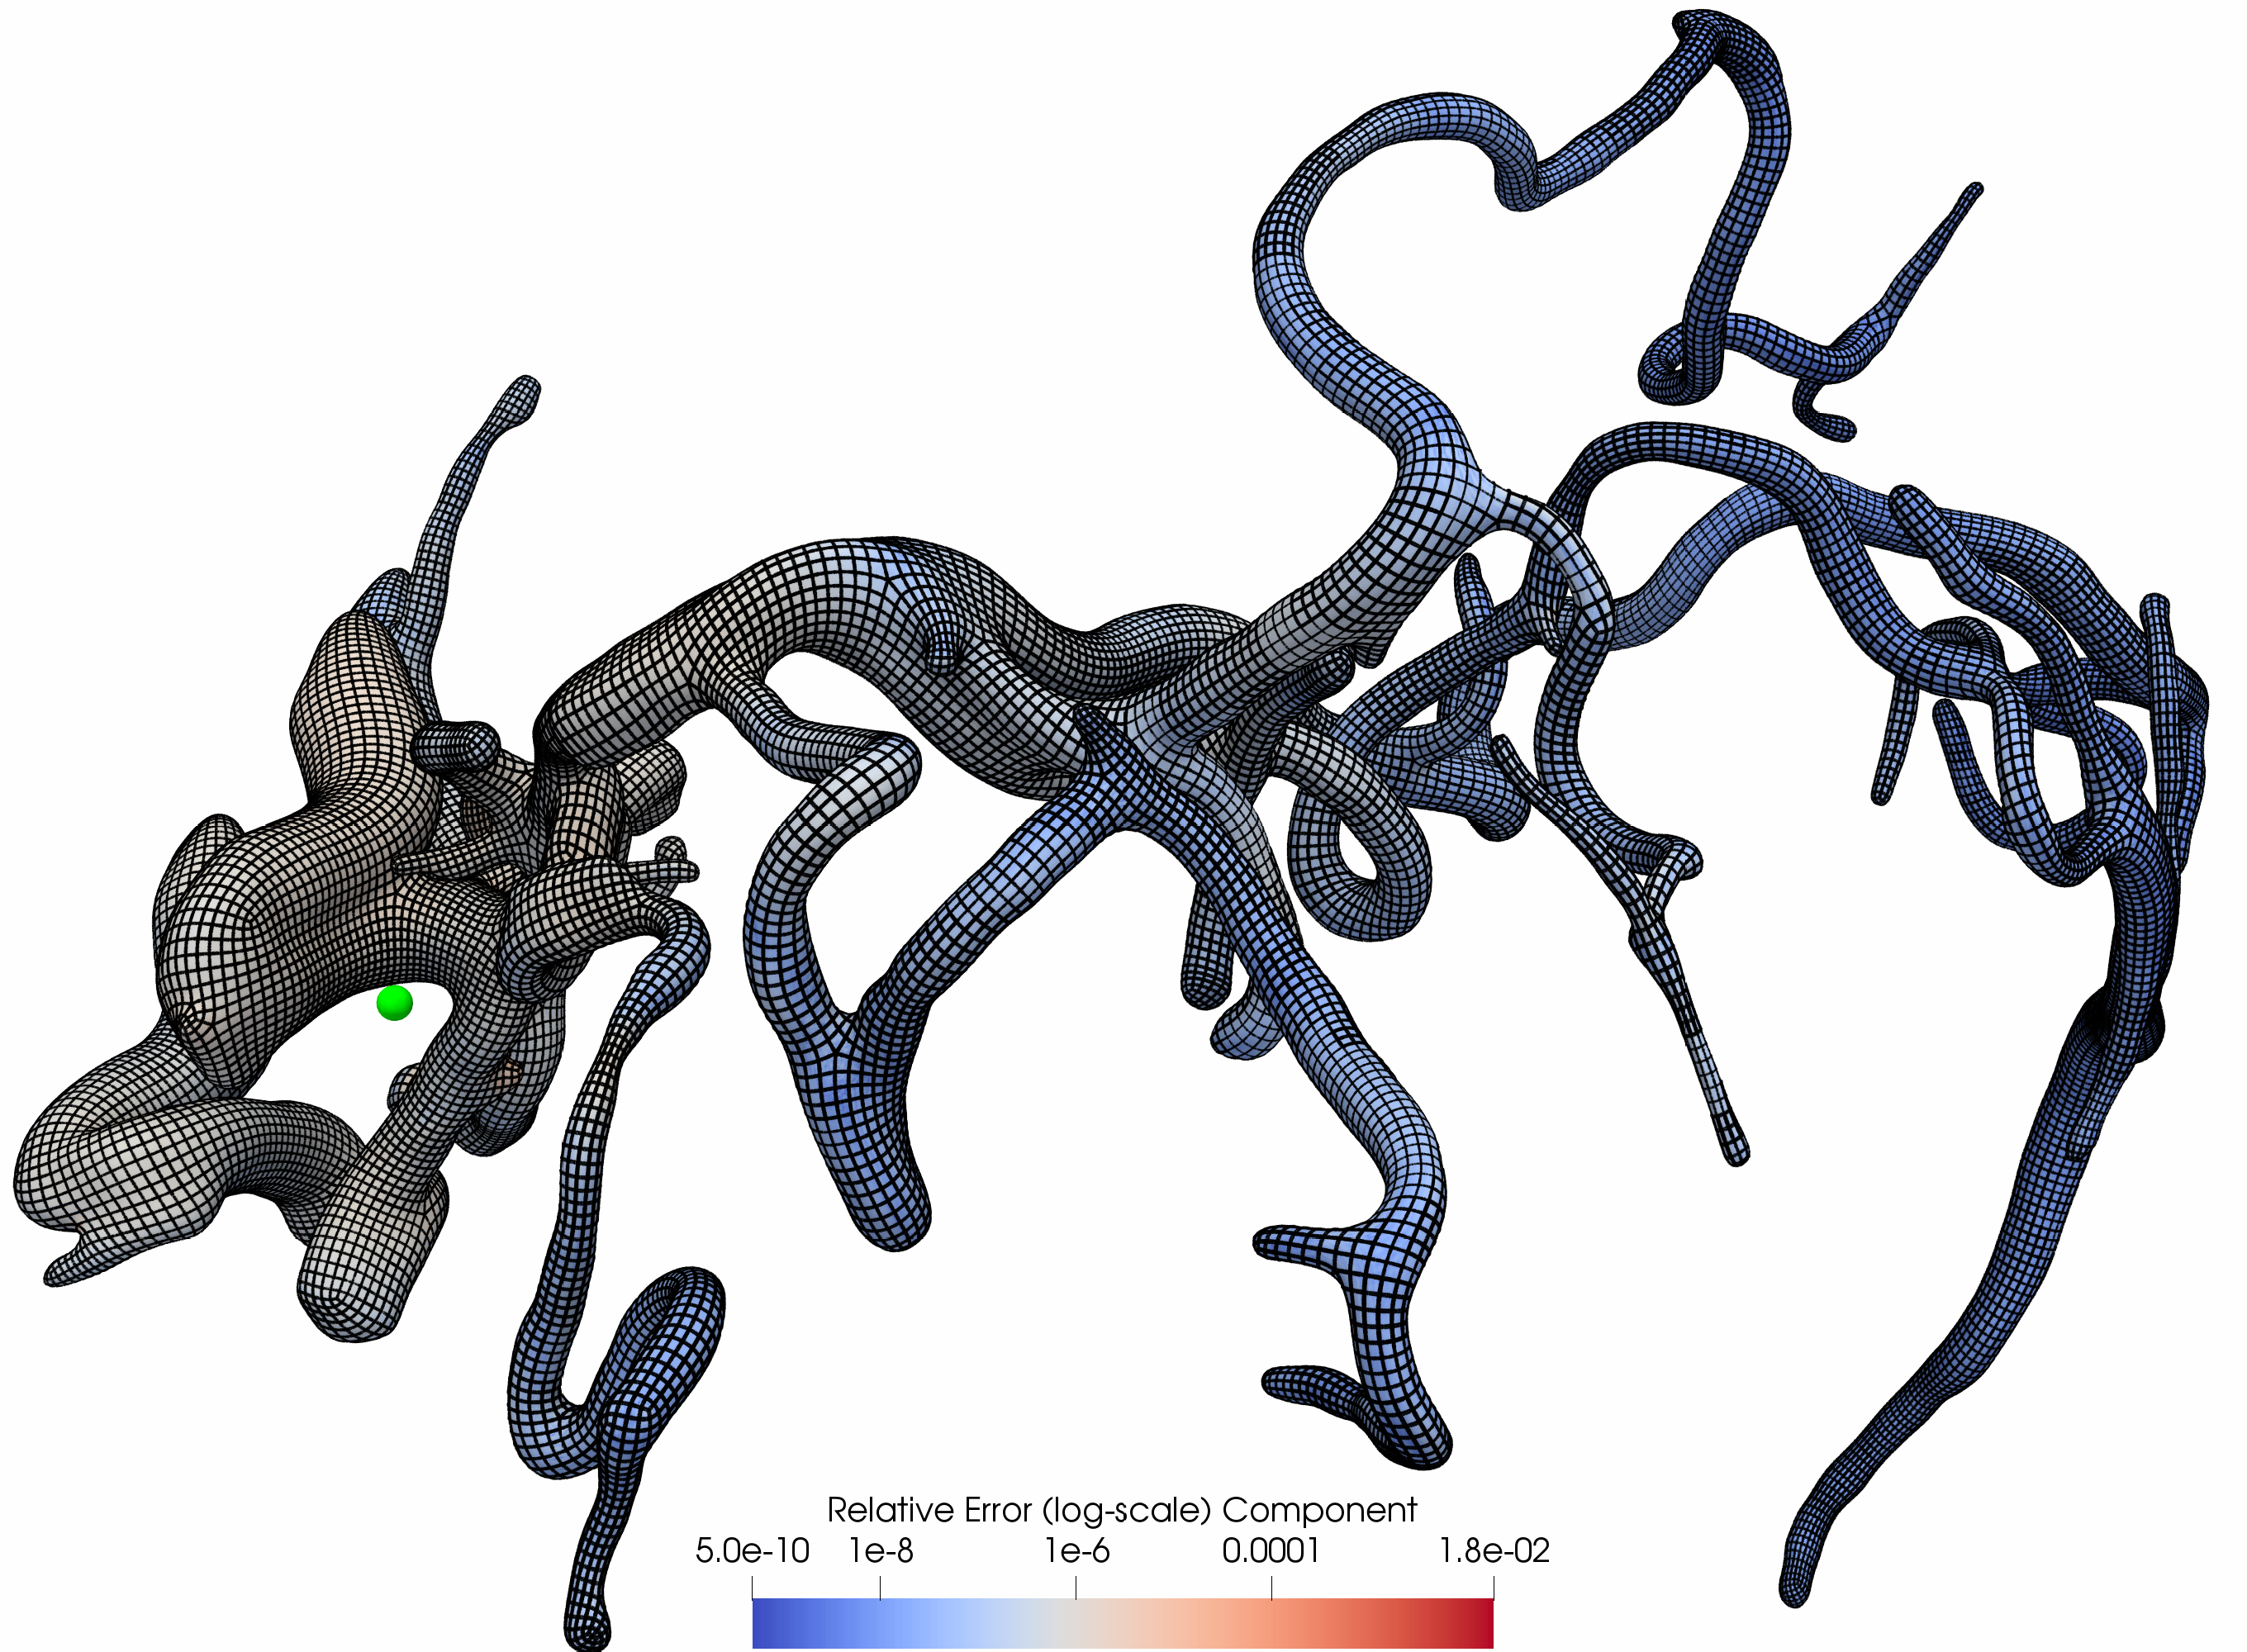
\includegraphics[width=\linewidth]{figs/largest_vessel_section.png}
  \end{minipage}\hfill
  \mcaption{fig:vessel}{Absolute error of \gmres solve via \qbkix on complex blood vessel geometry used in \cite{lu2019scalable}}{The blood vessel uses 40,960 8th order polynomial patches (black edges denote patch boundaries). The geometry is admissible by construction. 
    The point charge is located on left side of the figure (green)}
\end{figure}

We have demonstrated in \cite{lu2019scalable} a parallel implementation of \cref{sec:singular-eval}, applied to simulating red blood cell flows.
The surface geometry of the blood vessel shown in \cref{fig:vessel} is complex, with rapidly varying curvatures and geometric distortions due to singular vertices in the surface mesh.
Since the surface is admissible, we are able to apply parallel \qbkix directly without geometric preprocessing to solve an interior Dirichlet Stokes problem.
We use $a=.125$, $b=.125$, $p=6$ and $q=16$ as simulation parameters.

Using 32 machines each with twenty 2.6 Ghz cores with 100\abbrev{GB} of \abbrev{RAM}, we achieve a maximum pointwise error of $3\times 10^{-6}$ when solving a Stokes problem with constant density. 
We then place a random vector point charge two patch lengths away (relative to the patches in $\Pcoarse$) from the domain boundary (on the left side of \cref{fig:vessel}, solve \cref{eq:int-eq} using two-sided \qbkix, and evaluate the solution on the boundary using one-sided \qbkix.
The absolute error in the $\infty$-norm of the singular evaluation is plotted on the boundary surface.
There are 10,485,760 quadrature points in the coarse discretization, 167,772,160 quadrature points in the fine discretization, and 125,829,120 check points used in the two-sided \qbkix evaluation inside \gmres.
We evaluate the solved density at 209,715,200 points on the boundary with one-sided \qbkix to produce the render in \cref{fig:torii}.
We achieve a maximum pointwise error of $1.8\times 10^{-2}$ and can evaluate the singular integral at rate of 3529 target points per second per core. 
%The \gmres solve with two-sided \qbkix converged to \note[MJM]{X} in \note[MJM]{Y} iterations in \note[MJM]{Z} hours.


\section{Conclusion}


\chapter{Scalable Simulation of Red Blood Cell Flows in Complex Geometries}
\label{chp:bloodflow}
\section{Conclusion\label{sec:conclusion}}
We have presented \qbkix, a fast, high-order, kernel-independent, singular/near-singular quadrature scheme for elliptic boundary value problems in \threed on complex geometries defined by piecewise tensor-product polynomial surfaces.
%We detailed fast algorithms to enforce geometric conditions that ensure accurate singular/near-singular integration throughout the domain.
The primary advantage of our approach is \textit{algorithmic simplicity}: the algorithm can implemented easily with an existing smooth quadrature rule, a point \fmm and \oned and \twod interpolation schemes.
%We presented an error heuristic to trigger upsampling adaptively that incorporates varied surface curvature and is free of Newton iterations.
We presented fast geometry processing algorithms to guarantee accurate singular/near-singular integration, adaptively upsample the discretization and query local surface patches.
We then evaluated \qbkix in various test cases, for Laplace, Stokes, and elasticity problems on various patch-based geometries and compared our approach with \cite{YBZ}.

\cite{lu2019scalable} demonstrates a parallel implementation of \qbkix, but the geometric preprocessing and adaptive upsampling algorithms presented in \cref{sec:algo} are not parallelized.
This is a requirement to solve truly large-scale problems that exist in engineering applications.
Our method can also be easily restructured as a local method.
The comparison in \cref{sec:results-compare} highlights an important point: a local singular quadrature method can outperform a global method for moderate accuracies, \textit{even when the local scheme is asymptotically slower}.
This simple change can also dramatically improve both the serial performance and the parallel scalability of \qbkix shown in \cite{lu2019scalable}, due to the decreased communication of a smaller parallel \fmm evaluation.
The most important improvement to be made, however, is the equispaced extrapolation.
Constructing a superior extrapolation procedure, optimized for the boundary integral context, is the main focus of our current investigations.

\iffalse
\section{Acknowledgements}
We would like to thank Michael O'Neil, Dhairya Malhotra, Libin Lu, Alex Barnett, Leslie Greengard, Michael Shelley for insightful conversations, feedback and suggestions regarding this work. 
We would also like to thank the NYU HPC team, and Shenglong Wang in particular, for great support throughout the course of this work.
This work was supported by NSF grant DMS-1821334.
\fi


\chapter{Conclusion}
\label{chp:conclusion}
\section{Conclusion\label{sec:conclusion}}
We have presented \qbkix, a fast, high-order, kernel-independent, singular/near-singular quadrature scheme for elliptic boundary value problems in \threed on complex geometries defined by piecewise tensor-product polynomial surfaces.
%We detailed fast algorithms to enforce geometric conditions that ensure accurate singular/near-singular integration throughout the domain.
The primary advantage of our approach is \textit{algorithmic simplicity}: the algorithm can implemented easily with an existing smooth quadrature rule, a point \fmm and \oned and \twod interpolation schemes.
%We presented an error heuristic to trigger upsampling adaptively that incorporates varied surface curvature and is free of Newton iterations.
We presented fast geometry processing algorithms to guarantee accurate singular/near-singular integration, adaptively upsample the discretization and query local surface patches.
We then evaluated \qbkix in various test cases, for Laplace, Stokes, and elasticity problems on various patch-based geometries and compared our approach with \cite{YBZ}.

\cite{lu2019scalable} demonstrates a parallel implementation of \qbkix, but the geometric preprocessing and adaptive upsampling algorithms presented in \cref{sec:algo} are not parallelized.
This is a requirement to solve truly large-scale problems that exist in engineering applications.
Our method can also be easily restructured as a local method.
The comparison in \cref{sec:results-compare} highlights an important point: a local singular quadrature method can outperform a global method for moderate accuracies, \textit{even when the local scheme is asymptotically slower}.
This simple change can also dramatically improve both the serial performance and the parallel scalability of \qbkix shown in \cite{lu2019scalable}, due to the decreased communication of a smaller parallel \fmm evaluation.
The most important improvement to be made, however, is the equispaced extrapolation.
Constructing a superior extrapolation procedure, optimized for the boundary integral context, is the main focus of our current investigations.

\iffalse
\section{Acknowledgements}
We would like to thank Michael O'Neil, Dhairya Malhotra, Libin Lu, Alex Barnett, Leslie Greengard, Michael Shelley for insightful conversations, feedback and suggestions regarding this work. 
We would also like to thank the NYU HPC team, and Shenglong Wang in particular, for great support throughout the course of this work.
This work was supported by NSF grant DMS-1821334.
\fi



%% If your thesis has different "Parts", use commands such as the following:
%\part{First Part\label{part:one}}%
% \input{chap1}
%\input{chap2} % further chapters -- change file names to meaningful things...
%\input{chap3}
%\part{Second Part\label{part:two}}%
%\input{chap4}
%\input{chap5}
%\input{chap6}


%%%%% Appendices start %%%%%%%%%%%%%%%%
%% Comment out the following if your thesis has no appendix

\appendix

\chapter{Appendix}


\section{Kernels\label{app:kernels}}
Here we list the elliptic \pde's investigated in this work along with the associated kernels for their single- and double-layer potentials.
In this section, $\vx$ and $\vy$ are in $\mathbb{R}^3$, $\vx$ is the point of evaluation and $\vy$ is a point on the boundary and $\vr = \vx - \vy$. 
Recall that $\vn$ is the outward pointing unit normal at $\vy$ to the domain boundary $\Gamma$.
We denote the single layer kernel, also known as the \textit{fundamental solution} or \textit{Green's function} of the \pde, by $S$ and the double layer kernel by $D$.
\begin{enumerate}
  \item \textit{Laplace equation}:
    \begin{align*}
      &\Delta u = 0\\
      &S(\vx,\vy) = \frac{1}{4\pi}\frac{1}{\|\vr\|}, \quad 
      D(\vx, \vy) = - \frac{1}{4\pi} \frac{\vr \cdot \mathbf{n}}{\|\vr\|^3}
    \end{align*}
  \item \textit{Stokes equation}:
    \begin{align*}
      &\mu\Delta u - \nabla p = 0, \,\, \nabla \cdot u = 0\\
      &S(\vx,\vy) = \frac{1}{8\pi\mu}\left( \frac{1}{\|\vr\|} + \frac{\vr \otimes\vr}{\|\vr\|^3}\right), \quad 
      D(\vx, \vy) = - \frac{3}{4\mu\pi} \frac{\vr \otimes\vr}{\|\vr\|^5}(\vr \cdot \mathbf{n})
    \end{align*}
  \item \textit{Elasticity equation}:
    \begin{align*}
      &\mu\Delta u - \frac{\mu}{1-2\nu}\nabla(\nabla \cdot u) = 0\\
      &S(\vx,\vy) = \frac{1}{16\pi\mu(1-\nu)}\left( \frac{3-4\nu}{\|\vr\|} + \frac{\vr \otimes\vr}{\|\vr\|^3}\right), \\
      &D(\vx, \vy) = - \frac{1-2\nu}{8\mu(1-\nu)} \left(
      \frac{1}{\|\vr\|^3} \left(
      \vr \otimes \vn - (\vr\cdot\vn) I - \vn \otimes \vr 
      \right) - \frac{3}{1-2\nu}
      \frac{(\vr\cdot\vn) (\vr \otimes \vr)}{\|\vr\|^5}
      \right)
    \end{align*}
\end{enumerate}


\section{Computing the closest point on a patch  \label{app:closest_point}}
%\subsection{Optimization\label{app:closest_point_opt}}
%\begin{figure}%[!htb]
%  \centering
%    \includegraphics[width=.5\linewidth]{figs/newton-opt.pdf}
%    \mcaption{fig:newton-opt}{Closest point optimization schematic}{}
%\end{figure}
We include our algorithm to find the closest point $\vy$ on a patch $\vP$ to a point $\vx \in \mathbb{R}^3$ in the section for completeness.
For a surface or quadrature patch $\vP$ and point $\vx \in \mathbb{R}^3$, 
we need to compute a point $\vy = \vP(s^*, t^*)$ such that
\begin{equation}
  (s^*, t^*) = \argmin_{(s,t) \in [-1,1]^2} \|\vx - \vP(s,t)\|_2^2 =  \argmin_{(s,t) \in [-1,1]^2} \vr(s,t)\cdot \vr(s,t)
\end{equation}
where $ \vr = \vr(s,t) = \vx - \vP(s,t)$; let $g(s,t) = \vr\cdot \vr$.
We first consider the unconstrained problem
\begin{equation}
    (s^*, t^*) = \argmin_{(s,t) \in \mathbb{R}^2} \|\vx - \vP(s,t)\|_2^2  = \argmin_{(s,t) \in \mathbb{R}^2} \psi(s,t) 
\end{equation}
We solve this optimization problem with Newton's method.
The first and second derivatives of $\psi$ can be evaluated efficiently, since they are polynomials of fixed order.
The gradient and Hessian of the objective function are:
\begin{equation}
  \nabla \psi  =
  \begin{pmatrix}
    -\vP_s\cdot \vr \\
    -\vP_t\cdot \vr \\
  \end{pmatrix}, \quad
  %\label{eq:grad-newton} 
  \nabla^2 \psi = 
\begin{pmatrix}
  \vP_s \cdot \vP_s - \vr\cdot \vP_{ss} & \vP_s \cdot \vP_t - \vr\cdot \vP_{st}\\
  \vP_s \cdot \vP_t - \vr\cdot \vP_{st} & \vP_t \cdot \vP_t - \vr\cdot \vP_{tt}  \\
\end{pmatrix}.
  \label{equ:grad-hess-newton}
\end{equation}
The optimality conditions are 
\begin{equation}
\vP_s^* \cdot \vr^* = 0, \quad \vP_t^* \cdot \vr^* = 0, \quad (u,v) = (s^*, t^*).
  \label{eq:kkt}
\end{equation}
at a local optimum $(s^*, t^*)$.

Let $\psi_i = \psi(s_i,t_i)$, where $(s_i,t_i)$ is the value of the solution during the $i$th iteration of Newton's method.
To solve for the descent direction in Newton's method, we need to solve
\begin{equation}
  \nabla^2 \psi_i \, \eta_i = -\nabla \psi_i
  \label{eq:newton-system}
\end{equation}
where $\eta_i = (\Delta s_i,\Delta t_i)$ is the $i$th Newton update to $(s_i,t_i)$ such that
\begin{equation}
  s_{i+1} = \alpha_i\Delta s_i + s_i,\quad
  t_{i+1} = \alpha_i\Delta t_i + t_i
  \label{}
\end{equation}

We use four iterations of a backtracking line search with an Armijo condition to compute the step length $\alpha_i$ to ensure an appropriate size step is taken in case the initial guess is outside the region of quadratic convergence.
We compute the solution $(s^*, t^*)$ by iterating
\begin{equation}
  (s_n,t_n) = (s_{n-1}, t_{n-1}) + \alpha_{n-1} \eta_{n-1}, \quad \text{ while } \vP_s \cdot \vr > \err{opt}, \quad \vP_t \cdot \vr > \err{opt},
  \label{eq:descent_iter}
\end{equation}
until convergence, i.e., $\psi_i\approx \err{opt}$, $\vr \approx \vn(\vy)$.

If $(s^*, t^*) \in (-1,1)^2$, then the solution to the unconstrained problem is also the solution to the constrained problem.
However, if the closest point lies in $\mathbb{R}\setminus [-1,1]^2$, we need to ensure the inequality constraints are satisfied.
Additionally, if $(s^*, t^*)$ is on the boundary of $[-1,1]^2$, either $s^*$ or $t^*$ should be exactly zero; with the optimization scheme above, we can only claim that $|s^*| < \err{opt}$ (similarly for $t^*$).
To address both of these troubles, we can solve a one-dimensional projection of \cref{eq:newton-system} on to the boundary of $[-1,1]^2$.
For example, to find the closest point along the edge $v=0$, the Newton iteration becomes
\begin{equation}
  s_n = s_{n-1} + \alpha_{n-1}\frac{-\vP_s \cdot \vr}{\vP_s\cdot \vP_s - \vr\cdot \vP_{ss}},
  \label{eq:geom-newton-1d}
\end{equation}
where $\vP_s$, $\vP_{ss}$ and $\vr$ are evaluated at $s_{n-1}$.
Since the boundary is composed of $[-1,t], [1,t], [s,-1], [s,1]$ for $s,t\in[-1,1]$, we solve \cref{eq:geom-newton-1d} once for each interval.

This final algorithm to compute the closest point is as follows:
\begin{enumerate}
  \item We solve \cref{eq:newton-system} on an extended parameter domain $[-1-c, 1+c]^2$, and terminate the Newton iteration if $(s_i,t_i)$ walks outside this boundary. 
    If the Newton iteration terminates inside $[-1,1]^2$, then we've found the closest point.
    We typically choose $c = .2$.
  \item  If the solution is outside $[-1,1]^2$, we solve \cref{eq:newton-system} along each component of the boundary of $[-1,1]^2$, also on an extended parameter domain $[-1-c,1+c]$,
    by choosing an initial guess contained within the interval.
    The solution to these four problems that yields a minimal distance to $\vx$ to used as the closest point, if the solution is inside $[-1,1]$.
  \item If the closest point on the boundary is still outside of $[-1,1]^2$, the
      closest point to $\vx$ is chosen from $\vP(-1,-1), \vP(-1,1), \vP(1,-1),$ and $\vP(1,1)$ closest to $\vx$.
\end{enumerate}
This gives us an algorithm to compute the closest point on a quadrature patch $\vP$ to $\vx$.
The \oned and \twod Newton minimizations converge in ten iterations on average.




%% Note: If your thesis has more than one appendix, NYU requires a "list of
%% appendices" page before the body of the thesis. I don't provide the tools
%% to create that here, so you're on your own for that one... Sorry.


%%%% Input bibliography file %%%%%%%%%%%%%%%
%% For computer science dissertations, I'd recommend using the bibly package
%% to automatically create the .bib file from your citations:
%% https://github.com/michael-emmi/bibly

\cleardoublepage
\phantomsection
\bibliographystyle{apalike}
\addcontentsline{toc}{chapter}{Bibliography}

% \bibliography{dblp,references}

% The following is just for the sample template,
% I'd recommend deleting this and using the \bibliography command above
\bibliography{refs}


\end{document}

%%% Local Variables:
%%% mode: latex
%%% TeX-master: t
%%% End:
